\documentclass[sigplan,review,anonymous]{acmart}
\settopmatter{printfolios=true,printccs=false,printacmref=false}

\usepackage{amssymb,amsthm,amsmath}
\usepackage{graphicx}
\usepackage{lmodern}
\usepackage{textgreek}
\usepackage[utf8x]{inputenc}
\usepackage[LGR,TS1,T1]{fontenc}
\usepackage{comment}
\usepackage{tikz}
\usepackage{tikz-cd}
\usepackage[nocenter]{qtree}
\usepackage{fullpage}
\usepackage{hyperref}
\usepackage{multicol}
\usepackage{stmaryrd}
\usepackage{proof}
\usepackage{ucs}
\usepackage{agda}

%%

\newtheorem{theorem}{Theorem}[section]
\newtheorem{lemma}[theorem]{Lemma}
\newtheorem{definition}[theorem]{Definition}
\newtheorem{proposition}[theorem]{Proposition}
\newtheorem{corollary}[theorem]{Corollary}

\newcommand{\Gpd}{\ensuremath{\mathsf{Groupoid}}}
\newcommand{\nboxtimes}[2]{\,\,~{^{#1}\boxtimes^{#2}}~\,\,}
\newcommand{\mm}{\texttt{\textminus}}
\newcommand{\pp}{\texttt{+}}

\newcommand{\presumtype}{\uplus}
\newcommand{\preprodtype}{*}
\newcommand{\sumtype}{+}
\newcommand{\prodtype}{\times}
\newcommand{\fin}[1]{\ensuremath{\left[#1\right]}}
\newcommand{\Nat}{\ensuremath{\mathbb{N}}}

\newcommand{\inleft}[1]{\textsf{left}~#1}
\newcommand{\inright}[1]{\textsf{right}~#1}
\newcommand{\cp}[3]{#1\stackrel{#2}{\bullet}#3}
\newcommand{\idt}[3]{#2 \equiv_{#1} #3}
\newcommand{\idrt}[3]{#3 \equiv_{#1} #2}
\newcommand{\refl}[1]{\textsf{refl}~#1}
\newcommand{\alt}{~|~}
\newcommand{\linv}{l!}
\newcommand{\rinv}{r!}
\newcommand{\invinv}{!!}
\newcommand{\assoc}{\circ}
\newcommand{\identlp}{\ensuremath{\mathit{unite}_{\sumtype}\mathit{l}}}
\newcommand{\identrp}{\ensuremath{\mathit{uniti}_{\sumtype}\mathit{l}}}
\newcommand{\identlsp}{\ensuremath{\mathit{unite}_{\sumtype}\mathit{r}}}
\newcommand{\identrsp}{\ensuremath{\mathit{uniti}_{\sumtype}\mathit{r}}}
\newcommand{\swapp}{\ensuremath{\mathit{swap}_{\sumtype}}}
\newcommand{\assoclp}{\ensuremath{\mathit{assocl}_{\sumtype}}}
\newcommand{\assocrp}{\ensuremath{\mathit{assocr}_{\sumtype}}}
\newcommand{\identlt}{\ensuremath{\mathit{unite}_{\prodtype}\mathit{l}}}
\newcommand{\identrt}{\ensuremath{\mathit{uniti}_{\prodtype}\mathit{l}}}
\newcommand{\identlst}{\ensuremath{\mathit{unite}_{\prodtype}\mathit{r}}}
\newcommand{\identrst}{\ensuremath{\mathit{uniti}_{\prodtype}\mathit{r}}}
\newcommand{\swapt}{\ensuremath{\mathit{swap}_{\prodtype}}}
\newcommand{\assoclt}{\ensuremath{\mathit{assocl}_{\prodtype}}}
\newcommand{\assocrt}{\ensuremath{\mathit{assocr}_{\prodtype}}}
\newcommand{\absorbr}{\ensuremath{\mathit{absorbr}}}
\newcommand{\absorbl}{\ensuremath{\mathit{absorbl}}}
\newcommand{\factorzr}{\ensuremath{\mathit{factorzr}}}
\newcommand{\factorzl}{\ensuremath{\mathit{factorzl}}}
\newcommand{\dist}{\ensuremath{\mathit{dist}}}
\newcommand{\factor}{\ensuremath{\mathit{factor}}}
\newcommand{\distl}{\ensuremath{\mathit{distl}}}
\newcommand{\factorl}{\ensuremath{\mathit{factorl}}}
\newcommand{\iso}{\leftrightarrow}
\newcommand{\proves}{\vdash}
\newcommand{\idc}{\mathit{id}\!\!\leftrightarrow}
\newcommand{\Rule}[4]{
\makebox{{\rm #1}
$\displaystyle
\frac{\begin{array}{l}#2 \\\end{array}}
{\begin{array}{l}#3      \\\end{array}}$
 #4}}
\newcommand{\jdg}[3]{#2 \proves_{#1} #3}
\newcommand{\sem}[1]{\ensuremath{\llbracket{#1}\rrbracket}}

% Unicode declarations

%% \DeclareUnicodeCharacter{9678}{\ensuremath{\odot}}
%% \DeclareUnicodeCharacter{9636}{\ensuremath{\Box}}
%% shorten the longarrow
%% \DeclareUnicodeCharacter{10231}{\ensuremath{\leftrightarrow}}

\DeclareUnicodeCharacter{9679}{\ensuremath{\bullet}}
\DeclareUnicodeCharacter{8343}{\ensuremath{_l}}
\DeclareUnicodeCharacter{8337}{\ensuremath{_e}}
\DeclareUnicodeCharacter{8345}{\ensuremath{_n}}
\DeclareUnicodeCharacter{8347}{\ensuremath{_s}}
\DeclareUnicodeCharacter{8779}{\ensuremath{\approxeq}}
%% \newunicodechar{ℓ}{\ensuremath{\ell}}
%% \newunicodechar{⊔}{\ensuremath{\sqcup}}

\DeclareMathAlphabet{\mymathbb}{U}{bbold}{m}{n}

% TIKZ declarations
\tikzstyle{func}=[rectangle,draw,fill=black!20,minimum size=1.9em,
  text width=2.4em, text centered]

%%%%%%%%%%%%%%%%%%%%%%%%%%%%%%%%%%%%%%%%%%%%%%%%%%%%%%%%%%%%%%%%%%%%%%%%%%%%%%
%% Some needed unicode characters

% Convenient abbreviations
\newcommand{\AIC}[1]{\AgdaInductiveConstructor{#1}}

%%%%%%%%%%%%%%%%%%%%%%%%%%%%%%%%%%%%%%%%%%%%%%%%%%%%%%%%%%%%%%%%%%%%%%%%%%%%%%
%% Comments

%% \newif\ifcomments\commentstrue

%% \ifcomments
%% \newcommand{\authornote}[3]{\textcolor{#1}{[#3 ---#2]}}
%% \newcommand{\todo}[1]{\textcolor{red}{[TODO: #1]}}
%% \else
%% \newcommand{\authornote}[3]{}
%% \newcommand{\todo}[1]{}
%% \fi

%% %% \newcommand{\amr}[1]{}
%% %% \newcommand{\jc}[1]{}

%% \newcommand{\jc}[1]{\authornote{purple}{JC}{#1}}
%% \newcommand{\amr}[1]{\fbox{\begin{minipage}{0.9\textwidth}\color{red}{Amr says: {#1}}\end{minipage}}}
%%%%%%%%%%%%%%%%%%%%%%%%%%%%%%%%%%%%%%%%%%%%%%%%%%%%%%%%%%%%%%%%%%%%%%%%%%%%%%

% Not the final title!
% \title{Reversible Programming for the BX enthusiast}
%\title{Reversible programming applied to bidirectional programming}
\title{Optics and Type Equivalences}

\author{
Jacques Carette\\ Dept. of Computing and Software\\
        McMaster University \\ carette@mcmaster.ca
\and
Amr Sabry \\ Computer Science Dept.\\
        Indiana University \\ sabry@indiana.edu
}

\institution{}

\begin{document}
\maketitle

\begin{abstract}
Bidirectional programming, lenses, prisms, and other optics have connections
to reversible programming which have been explored from several perspectives,
mostly by attempting to recover bidirectional transformations from unidirectional
ones. We offer a novel and foundational perspective in which reversible programming
is expressed using “type equivalences.” This perspective offers several advantages:
first, it is possible to construct sets of sound and complete type equivalences
for certain collections of types; these correspond to canonical optic constructions.
Second, using ideas inspired by category theory and homotopy type theory,
it is possible to construct sound and complete “equivalences between equivalences”
which provide the canonical laws for reasoning about lens and prism equivalences.
\end{abstract}
\vskip 32pt

\AgdaHide{
\begin{code}%
\>[0]\AgdaSymbol{\{{-}\#}\AgdaSpace{}%
\AgdaKeyword{OPTIONS}\AgdaSpace{}%
\AgdaOption{{-}{-}without{-}K}\AgdaSpace{}%
\AgdaSymbol{\#{-}\}}\<%
\\
\>[0]\AgdaKeyword{module}\AgdaSpace{}%
\AgdaModule{RCforBX}\AgdaSpace{}%
\AgdaKeyword{where}\<%
\\
%
\\[\AgdaEmptyExtraSkip]%
\>[0]\AgdaKeyword{open}\AgdaSpace{}%
\AgdaKeyword{import}\AgdaSpace{}%
\AgdaModule{Level}\<%
\\
\>[0]\AgdaKeyword{open}\AgdaSpace{}%
\AgdaKeyword{import}\AgdaSpace{}%
\AgdaModule{Data.Product}\AgdaSpace{}%
\AgdaKeyword{using}\AgdaSpace{}%
\AgdaSymbol{(}\AgdaOperator{\AgdaFunction{\AgdaUnderscore{}×\AgdaUnderscore{}}}\AgdaSymbol{;}\AgdaSpace{}%
\AgdaOperator{\AgdaInductiveConstructor{\AgdaUnderscore{},\AgdaUnderscore{}}}\AgdaSymbol{;}\AgdaSpace{}%
\AgdaField{proj₁}\AgdaSymbol{;}\AgdaSpace{}%
\AgdaField{proj₂}\AgdaSymbol{;}\AgdaSpace{}%
\AgdaRecord{Σ}\AgdaSymbol{)}\<%
\\
\>[0][@{}l@{\AgdaIndent{0}}]%
\>[2]\AgdaKeyword{renaming}\AgdaSpace{}%
\AgdaSymbol{(}\AgdaFunction{map}\AgdaSpace{}%
\AgdaSymbol{to}\AgdaSpace{}%
\AgdaFunction{map×}\AgdaSymbol{)}\<%
\\
\>[0]\AgdaKeyword{open}\AgdaSpace{}%
\AgdaKeyword{import}\AgdaSpace{}%
\AgdaModule{Data.Sum}\AgdaSpace{}%
\AgdaKeyword{using}\AgdaSpace{}%
\AgdaSymbol{(}\AgdaOperator{\AgdaDatatype{\AgdaUnderscore{}⊎\AgdaUnderscore{}}}\AgdaSymbol{;}\AgdaSpace{}%
\AgdaInductiveConstructor{inj₁}\AgdaSymbol{;}\AgdaSpace{}%
\AgdaInductiveConstructor{inj₂}\AgdaSymbol{;}\AgdaSpace{}%
\AgdaOperator{\AgdaFunction{[\AgdaUnderscore{},\AgdaUnderscore{}]′}}\AgdaSymbol{)}\<%
\\
\>[0]\AgdaKeyword{open}\AgdaSpace{}%
\AgdaKeyword{import}\AgdaSpace{}%
\AgdaModule{Data.Sum.Properties}\<%
\\
\>[0]\AgdaKeyword{open}\AgdaSpace{}%
\AgdaKeyword{import}\AgdaSpace{}%
\AgdaModule{Data.Unit}\<%
\\
\>[0]\AgdaKeyword{open}\AgdaSpace{}%
\AgdaKeyword{import}\AgdaSpace{}%
\AgdaModule{Data.Empty}\<%
\\
\>[0]\AgdaKeyword{open}\AgdaSpace{}%
\AgdaKeyword{import}\AgdaSpace{}%
\AgdaModule{Data.Maybe}\<%
\\
\>[0]\AgdaKeyword{open}\AgdaSpace{}%
\AgdaKeyword{import}\AgdaSpace{}%
\AgdaModule{Relation.Binary.PropositionalEquality}\AgdaSpace{}%
\AgdaSymbol{as}\AgdaSpace{}%
\AgdaModule{P}\<%
\\
\>[0][@{}l@{\AgdaIndent{0}}]%
\>[2]\AgdaKeyword{using}\AgdaSpace{}%
\AgdaSymbol{(}\AgdaOperator{\AgdaDatatype{\AgdaUnderscore{}≡\AgdaUnderscore{}}}\AgdaSymbol{;}\AgdaSpace{}%
\AgdaFunction{cong}\AgdaSymbol{;}\AgdaSpace{}%
\AgdaFunction{cong₂}\AgdaSymbol{;}\AgdaSpace{}%
\AgdaFunction{sym}\AgdaSymbol{;}\AgdaSpace{}%
\AgdaFunction{trans}\AgdaSymbol{;}\AgdaSpace{}%
\AgdaInductiveConstructor{refl}\AgdaSymbol{;}\AgdaSpace{}%
\AgdaFunction{inspect}\AgdaSymbol{;}\AgdaSpace{}%
\AgdaOperator{\AgdaInductiveConstructor{[\AgdaUnderscore{}]}}\AgdaSymbol{)}\<%
\\
\>[0]\AgdaKeyword{open}\AgdaSpace{}%
\AgdaKeyword{import}\AgdaSpace{}%
\AgdaModule{Function}\AgdaSpace{}%
\AgdaKeyword{using}\AgdaSpace{}%
\AgdaSymbol{(}\AgdaFunction{id}\AgdaSymbol{;}\AgdaSpace{}%
\AgdaFunction{const}\AgdaSymbol{;}\AgdaSpace{}%
\AgdaOperator{\AgdaFunction{\AgdaUnderscore{}∘\AgdaUnderscore{}}}\AgdaSymbol{;}\AgdaSpace{}%
\AgdaOperator{\AgdaFunction{case\AgdaUnderscore{}of\AgdaUnderscore{}}}\AgdaSymbol{;}\AgdaSpace{}%
\AgdaOperator{\AgdaFunction{\AgdaUnderscore{}∋\AgdaUnderscore{}}}\AgdaSymbol{)}\<%
\\
%
\\[\AgdaEmptyExtraSkip]%
\>[0]\AgdaKeyword{open}\AgdaSpace{}%
\AgdaKeyword{import}\AgdaSpace{}%
\AgdaModule{Relation.Binary}\AgdaSpace{}%
\AgdaKeyword{using}\AgdaSpace{}%
\AgdaSymbol{(}\AgdaRecord{Setoid}\AgdaSymbol{;}\AgdaSpace{}%
\AgdaFunction{Rel}\AgdaSymbol{)}\<%
\\
\>[0]\AgdaKeyword{open}\AgdaSpace{}%
\AgdaKeyword{import}\AgdaSpace{}%
\AgdaModule{Function.Equality}\AgdaSpace{}%
\AgdaKeyword{using}\AgdaSpace{}%
\AgdaSymbol{(}\AgdaOperator{\AgdaField{\AgdaUnderscore{}⟨\$⟩\AgdaUnderscore{}}}\AgdaSymbol{;}\AgdaSpace{}%
\AgdaRecord{Π}\AgdaSymbol{)}\<%
\\
\>[0]\AgdaComment{{-}{-} open import Relation.Binary.Product.Pointwise using (\AgdaUnderscore{}×{-}setoid\AgdaUnderscore{})}\<%
\\
\>[0]\AgdaComment{{-}{-} open import Data.Product.Relation.Pointwise.NonDependent using (\AgdaUnderscore{}×{-}inverse\AgdaUnderscore{})}\<%
\\
\>[0]\AgdaKeyword{open}\AgdaSpace{}%
\AgdaKeyword{import}\AgdaSpace{}%
\AgdaModule{Function.Inverse}\AgdaSpace{}%
\AgdaKeyword{using}\AgdaSpace{}%
\AgdaSymbol{(}\AgdaRecord{Inverse}\AgdaSymbol{)}\<%
\\
\>[0][@{}l@{\AgdaIndent{0}}]%
\>[2]\AgdaKeyword{renaming}\AgdaSpace{}%
\AgdaSymbol{(}\AgdaFunction{id}\AgdaSpace{}%
\AgdaSymbol{to}\AgdaSpace{}%
\AgdaFunction{idF}\AgdaSymbol{;}\AgdaSpace{}%
\AgdaOperator{\AgdaFunction{\AgdaUnderscore{}∘\AgdaUnderscore{}}}\AgdaSpace{}%
\AgdaSymbol{to}\AgdaSpace{}%
\AgdaOperator{\AgdaFunction{\AgdaUnderscore{}∘F\AgdaUnderscore{}}}\AgdaSymbol{)}\<%
\\
\>[0]\AgdaKeyword{open}\AgdaSpace{}%
\AgdaModule{Inverse}\AgdaSpace{}%
\AgdaKeyword{using}\AgdaSpace{}%
\AgdaSymbol{(}\AgdaField{to}\AgdaSymbol{;}\AgdaSpace{}%
\AgdaField{from}\AgdaSymbol{;}\AgdaSpace{}%
\AgdaFunction{left{-}inverse{-}of}\AgdaSymbol{;}\AgdaSpace{}%
\AgdaFunction{right{-}inverse{-}of}\AgdaSymbol{)}\<%
\\
%
\\[\AgdaEmptyExtraSkip]%
\>[0]\AgdaKeyword{open}\AgdaSpace{}%
\AgdaKeyword{import}\AgdaSpace{}%
\AgdaModule{Equiv}\<%
\\
\>[0]\AgdaKeyword{open}\AgdaSpace{}%
\AgdaKeyword{import}\AgdaSpace{}%
\AgdaModule{TypeEquiv}\<%
\\
\>[0]\AgdaKeyword{open}\AgdaSpace{}%
\AgdaKeyword{import}\AgdaSpace{}%
\AgdaModule{EquivEquiv}\<%
\\
%
\\[\AgdaEmptyExtraSkip]%
\>[0]\AgdaComment{{-}{-} Do our own Setoid product, because the built{-}in one triggers an internal error!}\<%
\\
\>[0]\AgdaOperator{\AgdaFunction{\AgdaUnderscore{}×S\AgdaUnderscore{}}}\AgdaSpace{}%
\AgdaSymbol{:}\AgdaSpace{}%
\AgdaSymbol{\{}\AgdaBound{a}\AgdaSpace{}%
\AgdaBound{b}\AgdaSpace{}%
\AgdaBound{c}\AgdaSpace{}%
\AgdaBound{d}\AgdaSpace{}%
\AgdaSymbol{:}\AgdaSpace{}%
\AgdaPostulate{Level}\AgdaSymbol{\}}\AgdaSpace{}%
\AgdaSymbol{→}\AgdaSpace{}%
\AgdaRecord{Setoid}\AgdaSpace{}%
\AgdaBound{a}\AgdaSpace{}%
\AgdaBound{b}\AgdaSpace{}%
\AgdaSymbol{→}\AgdaSpace{}%
\AgdaRecord{Setoid}\AgdaSpace{}%
\AgdaBound{c}\AgdaSpace{}%
\AgdaBound{d}\AgdaSpace{}%
\AgdaSymbol{→}\AgdaSpace{}%
\AgdaRecord{Setoid}\AgdaSpace{}%
\AgdaSymbol{(}\AgdaBound{a}\AgdaSpace{}%
\AgdaOperator{\AgdaPrimitive{⊔}}\AgdaSpace{}%
\AgdaBound{c}\AgdaSymbol{)}\AgdaSpace{}%
\AgdaSymbol{(}\AgdaBound{b}\AgdaSpace{}%
\AgdaOperator{\AgdaPrimitive{⊔}}\AgdaSpace{}%
\AgdaBound{d}\AgdaSymbol{)}\<%
\\
\>[0]\AgdaBound{S}%
\>[108I]\AgdaOperator{\AgdaFunction{×S}}\AgdaSpace{}%
\AgdaBound{T}\AgdaSpace{}%
\AgdaSymbol{=}\AgdaSpace{}%
\AgdaKeyword{record}\<%
\\
\>[.]\<[108I]%
\>[2]\AgdaSymbol{\{}\AgdaSpace{}%
\AgdaField{Carrier}\AgdaSpace{}%
\AgdaSymbol{=}\AgdaSpace{}%
\AgdaField{Setoid.Carrier}\AgdaSpace{}%
\AgdaBound{S}\AgdaSpace{}%
\AgdaOperator{\AgdaFunction{×}}\AgdaSpace{}%
\AgdaField{Setoid.Carrier}\AgdaSpace{}%
\AgdaBound{T}\<%
\\
%
\>[2]\AgdaSymbol{;}\AgdaSpace{}%
\AgdaOperator{\AgdaField{\AgdaUnderscore{}≈\AgdaUnderscore{}}}\AgdaSpace{}%
\AgdaSymbol{=}\AgdaSpace{}%
\AgdaSymbol{λ}\AgdaSpace{}%
\AgdaSymbol{\{(}\AgdaBound{s₁}\AgdaSpace{}%
\AgdaOperator{\AgdaInductiveConstructor{,}}\AgdaSpace{}%
\AgdaBound{t₁}\AgdaSymbol{)}\AgdaSpace{}%
\AgdaSymbol{(}\AgdaBound{s₂}\AgdaSpace{}%
\AgdaOperator{\AgdaInductiveConstructor{,}}\AgdaSpace{}%
\AgdaBound{t₂}\AgdaSymbol{)}\AgdaSpace{}%
\AgdaSymbol{→}\AgdaSpace{}%
\AgdaOperator{\AgdaField{Setoid.\AgdaUnderscore{}≈\AgdaUnderscore{}}}\AgdaSpace{}%
\AgdaBound{S}\AgdaSpace{}%
\AgdaBound{s₁}\AgdaSpace{}%
\AgdaBound{s₂}\AgdaSpace{}%
\AgdaOperator{\AgdaFunction{×}}\AgdaSpace{}%
\AgdaOperator{\AgdaField{Setoid.\AgdaUnderscore{}≈\AgdaUnderscore{}}}\AgdaSpace{}%
\AgdaBound{T}\AgdaSpace{}%
\AgdaBound{t₁}\AgdaSpace{}%
\AgdaBound{t₂}\AgdaSymbol{\}}\<%
\\
%
\>[2]\AgdaSymbol{;}%
\>[138I]\AgdaField{isEquivalence}\AgdaSpace{}%
\AgdaSymbol{=}\AgdaSpace{}%
\AgdaKeyword{record}\<%
\\
\>[.]\<[138I]%
\>[4]\AgdaSymbol{\{}\AgdaSpace{}%
\AgdaField{refl}\AgdaSpace{}%
\AgdaSymbol{=}\AgdaSpace{}%
\AgdaSymbol{(}\AgdaFunction{Setoid.refl}\AgdaSpace{}%
\AgdaBound{S}\AgdaSymbol{)}\AgdaSpace{}%
\AgdaOperator{\AgdaInductiveConstructor{,}}\AgdaSpace{}%
\AgdaSymbol{(}\AgdaFunction{Setoid.refl}\AgdaSpace{}%
\AgdaBound{T}\AgdaSymbol{)}\<%
\\
%
\>[4]\AgdaSymbol{;}\AgdaSpace{}%
\AgdaField{sym}\AgdaSpace{}%
\AgdaSymbol{=}\AgdaSpace{}%
\AgdaSymbol{λ}\AgdaSpace{}%
\AgdaBound{pf}\AgdaSpace{}%
\AgdaSymbol{→}\AgdaSpace{}%
\AgdaFunction{Setoid.sym}\AgdaSpace{}%
\AgdaBound{S}\AgdaSpace{}%
\AgdaSymbol{(}\AgdaField{proj₁}\AgdaSpace{}%
\AgdaBound{pf}\AgdaSymbol{)}\AgdaSpace{}%
\AgdaOperator{\AgdaInductiveConstructor{,}}\AgdaSpace{}%
\AgdaFunction{Setoid.sym}\AgdaSpace{}%
\AgdaBound{T}\AgdaSpace{}%
\AgdaSymbol{(}\AgdaField{proj₂}\AgdaSpace{}%
\AgdaBound{pf}\AgdaSymbol{)}\<%
\\
%
\>[4]\AgdaSymbol{;}\AgdaSpace{}%
\AgdaField{trans}\AgdaSpace{}%
\AgdaSymbol{=}\AgdaSpace{}%
\AgdaSymbol{λ}\AgdaSpace{}%
\AgdaSymbol{\{(}\AgdaBound{i≈Sj}\AgdaSpace{}%
\AgdaOperator{\AgdaInductiveConstructor{,}}\AgdaSpace{}%
\AgdaBound{i≈Tj}\AgdaSymbol{)}\AgdaSpace{}%
\AgdaSymbol{(}\AgdaBound{j≈Sk}\AgdaSpace{}%
\AgdaOperator{\AgdaInductiveConstructor{,}}\AgdaSpace{}%
\AgdaBound{j≈Tk}\AgdaSymbol{)}\AgdaSpace{}%
\AgdaSymbol{→}\AgdaSpace{}%
\AgdaFunction{Setoid.trans}\AgdaSpace{}%
\AgdaBound{S}\AgdaSpace{}%
\AgdaBound{i≈Sj}\AgdaSpace{}%
\AgdaBound{j≈Sk}\AgdaSpace{}%
\AgdaOperator{\AgdaInductiveConstructor{,}}\AgdaSpace{}%
\AgdaFunction{Setoid.trans}\AgdaSpace{}%
\AgdaBound{T}\AgdaSpace{}%
\AgdaBound{i≈Tj}\AgdaSpace{}%
\AgdaBound{j≈Tk}\AgdaSpace{}%
\AgdaSymbol{\}}\<%
\\
%
\>[4]\AgdaSymbol{\}}\AgdaSpace{}%
\AgdaSymbol{\}}\<%
\\
%
\\[\AgdaEmptyExtraSkip]%
\>[0]\AgdaOperator{\AgdaFunction{\AgdaUnderscore{}≈S\AgdaUnderscore{}}}\AgdaSpace{}%
\AgdaSymbol{:}\AgdaSpace{}%
\AgdaSymbol{\{}\AgdaBound{a}\AgdaSpace{}%
\AgdaBound{b}\AgdaSpace{}%
\AgdaSymbol{:}\AgdaSpace{}%
\AgdaPostulate{Level}\AgdaSymbol{\}}\AgdaSpace{}%
\AgdaSymbol{→}\AgdaSpace{}%
\AgdaSymbol{(}\AgdaBound{A}\AgdaSpace{}%
\AgdaSymbol{:}\AgdaSpace{}%
\AgdaRecord{Setoid}\AgdaSpace{}%
\AgdaBound{a}\AgdaSpace{}%
\AgdaBound{b}\AgdaSymbol{)}\AgdaSpace{}%
\AgdaSymbol{→}\AgdaSpace{}%
\AgdaSymbol{(}\AgdaBound{B}\AgdaSpace{}%
\AgdaSymbol{:}\AgdaSpace{}%
\AgdaRecord{Setoid}\AgdaSpace{}%
\AgdaBound{a}\AgdaSpace{}%
\AgdaBound{b}\AgdaSymbol{)}\AgdaSpace{}%
\AgdaSymbol{→}\AgdaSpace{}%
\AgdaFunction{Rel}\AgdaSpace{}%
\AgdaSymbol{(}\AgdaField{Setoid.Carrier}\AgdaSpace{}%
\AgdaBound{A}\AgdaSpace{}%
\AgdaOperator{\AgdaDatatype{⊎}}\AgdaSpace{}%
\AgdaField{Setoid.Carrier}\AgdaSpace{}%
\AgdaBound{B}\AgdaSymbol{)}\AgdaSpace{}%
\AgdaBound{b}\<%
\\
\>[0]\AgdaSymbol{(}\AgdaBound{S}\AgdaSpace{}%
\AgdaOperator{\AgdaFunction{≈S}}\AgdaSpace{}%
\AgdaBound{T}\AgdaSymbol{)}\AgdaSpace{}%
\AgdaSymbol{(}\AgdaInductiveConstructor{inj₁}\AgdaSpace{}%
\AgdaBound{x}\AgdaSymbol{)}\AgdaSpace{}%
\AgdaSymbol{(}\AgdaInductiveConstructor{inj₁}\AgdaSpace{}%
\AgdaBound{x₁}\AgdaSymbol{)}\AgdaSpace{}%
\AgdaSymbol{=}\AgdaSpace{}%
\AgdaOperator{\AgdaField{Setoid.\AgdaUnderscore{}≈\AgdaUnderscore{}}}\AgdaSpace{}%
\AgdaBound{S}\AgdaSpace{}%
\AgdaBound{x}\AgdaSpace{}%
\AgdaBound{x₁}\<%
\\
\>[0]\AgdaSymbol{(}\AgdaOperator{\AgdaFunction{\AgdaUnderscore{}≈S\AgdaUnderscore{}}}\AgdaSpace{}%
\AgdaSymbol{\{\AgdaUnderscore{}\}}\AgdaSpace{}%
\AgdaSymbol{\{}\AgdaBound{b}\AgdaSymbol{\}}\AgdaSpace{}%
\AgdaBound{S}\AgdaSpace{}%
\AgdaBound{T}\AgdaSymbol{)}\AgdaSpace{}%
\AgdaSymbol{(}\AgdaInductiveConstructor{inj₁}\AgdaSpace{}%
\AgdaBound{x}\AgdaSymbol{)}\AgdaSpace{}%
\AgdaSymbol{(}\AgdaInductiveConstructor{inj₂}\AgdaSpace{}%
\AgdaBound{y}\AgdaSymbol{)}\AgdaSpace{}%
\AgdaSymbol{=}\AgdaSpace{}%
\AgdaRecord{Lift}\AgdaSpace{}%
\AgdaBound{b}\AgdaSpace{}%
\AgdaDatatype{⊥}\<%
\\
\>[0]\AgdaSymbol{(}\AgdaOperator{\AgdaFunction{\AgdaUnderscore{}≈S\AgdaUnderscore{}}}\AgdaSpace{}%
\AgdaSymbol{\{\AgdaUnderscore{}\}}\AgdaSpace{}%
\AgdaSymbol{\{}\AgdaBound{b}\AgdaSymbol{\}}\AgdaSpace{}%
\AgdaBound{S}\AgdaSpace{}%
\AgdaBound{T}\AgdaSymbol{)}\AgdaSpace{}%
\AgdaSymbol{(}\AgdaInductiveConstructor{inj₂}\AgdaSpace{}%
\AgdaBound{y₁}\AgdaSymbol{)}\AgdaSpace{}%
\AgdaSymbol{(}\AgdaInductiveConstructor{inj₁}\AgdaSpace{}%
\AgdaBound{x}\AgdaSymbol{)}\AgdaSpace{}%
\AgdaSymbol{=}\AgdaSpace{}%
\AgdaRecord{Lift}\AgdaSpace{}%
\AgdaBound{b}\AgdaSpace{}%
\AgdaDatatype{⊥}\<%
\\
\>[0]\AgdaSymbol{(}\AgdaBound{S}\AgdaSpace{}%
\AgdaOperator{\AgdaFunction{≈S}}\AgdaSpace{}%
\AgdaBound{T}\AgdaSymbol{)}\AgdaSpace{}%
\AgdaSymbol{(}\AgdaInductiveConstructor{inj₂}\AgdaSpace{}%
\AgdaBound{y₁}\AgdaSymbol{)}\AgdaSpace{}%
\AgdaSymbol{(}\AgdaInductiveConstructor{inj₂}\AgdaSpace{}%
\AgdaBound{y}\AgdaSymbol{)}\AgdaSpace{}%
\AgdaSymbol{=}\AgdaSpace{}%
\AgdaOperator{\AgdaField{Setoid.\AgdaUnderscore{}≈\AgdaUnderscore{}}}\AgdaSpace{}%
\AgdaBound{T}\AgdaSpace{}%
\AgdaBound{y₁}\AgdaSpace{}%
\AgdaBound{y}\<%
\\
%
\\[\AgdaEmptyExtraSkip]%
\>[0]\AgdaOperator{\AgdaFunction{\AgdaUnderscore{}⊎S\AgdaUnderscore{}}}\AgdaSpace{}%
\AgdaSymbol{:}\AgdaSpace{}%
\AgdaSymbol{\{}\AgdaBound{a}\AgdaSpace{}%
\AgdaBound{b}\AgdaSpace{}%
\AgdaSymbol{:}\AgdaSpace{}%
\AgdaPostulate{Level}\AgdaSymbol{\}}\AgdaSpace{}%
\AgdaSymbol{→}\AgdaSpace{}%
\AgdaRecord{Setoid}\AgdaSpace{}%
\AgdaBound{a}\AgdaSpace{}%
\AgdaBound{b}\AgdaSpace{}%
\AgdaSymbol{→}\AgdaSpace{}%
\AgdaRecord{Setoid}\AgdaSpace{}%
\AgdaBound{a}\AgdaSpace{}%
\AgdaBound{b}\AgdaSpace{}%
\AgdaSymbol{→}\AgdaSpace{}%
\AgdaRecord{Setoid}\AgdaSpace{}%
\AgdaBound{a}\AgdaSpace{}%
\AgdaBound{b}\<%
\\
\>[0]\AgdaOperator{\AgdaFunction{\AgdaUnderscore{}⊎S\AgdaUnderscore{}}}\AgdaSpace{}%
\AgdaSymbol{\{}\AgdaBound{a}\AgdaSymbol{\}}\AgdaSpace{}%
\AgdaSymbol{\{}\AgdaBound{b}\AgdaSymbol{\}}\AgdaSpace{}%
\AgdaBound{S}\AgdaSpace{}%
\AgdaBound{T}\AgdaSpace{}%
\AgdaSymbol{=}\AgdaSpace{}%
\AgdaKeyword{record}\<%
\\
\>[0][@{}l@{\AgdaIndent{0}}]%
\>[2]\AgdaSymbol{\{}\AgdaSpace{}%
\AgdaField{Carrier}\AgdaSpace{}%
\AgdaSymbol{=}\AgdaSpace{}%
\AgdaField{Carrier}\AgdaSpace{}%
\AgdaBound{S}\AgdaSpace{}%
\AgdaOperator{\AgdaDatatype{⊎}}\AgdaSpace{}%
\AgdaField{Carrier}\AgdaSpace{}%
\AgdaBound{T}\<%
\\
%
\>[2]\AgdaSymbol{;}\AgdaSpace{}%
\AgdaOperator{\AgdaField{\AgdaUnderscore{}≈\AgdaUnderscore{}}}\AgdaSpace{}%
\AgdaSymbol{=}\AgdaSpace{}%
\AgdaBound{S}\AgdaSpace{}%
\AgdaOperator{\AgdaFunction{≈S}}\AgdaSpace{}%
\AgdaBound{T}\<%
\\
%
\>[2]\AgdaSymbol{;}%
\>[289I]\AgdaField{isEquivalence}\AgdaSpace{}%
\AgdaSymbol{=}\AgdaSpace{}%
\AgdaKeyword{record}\<%
\\
\>[.]\<[289I]%
\>[4]\AgdaSymbol{\{}\AgdaSpace{}%
\AgdaField{refl}\AgdaSpace{}%
\AgdaSymbol{=}\AgdaSpace{}%
\AgdaSymbol{λ}\AgdaSpace{}%
\AgdaSymbol{\{}\AgdaSpace{}%
\AgdaSymbol{\{}\AgdaInductiveConstructor{inj₁}\AgdaSpace{}%
\AgdaBound{x}\AgdaSymbol{\}}\AgdaSpace{}%
\AgdaSymbol{→}\AgdaSpace{}%
\AgdaFunction{Setoid.refl}\AgdaSpace{}%
\AgdaBound{S}\AgdaSpace{}%
\AgdaSymbol{;}\AgdaSpace{}%
\AgdaSymbol{\{}\AgdaInductiveConstructor{inj₂}\AgdaSpace{}%
\AgdaBound{y}\AgdaSymbol{\}}\AgdaSpace{}%
\AgdaSymbol{→}\AgdaSpace{}%
\AgdaFunction{Setoid.refl}\AgdaSpace{}%
\AgdaBound{T}\AgdaSymbol{\}}\<%
\\
%
\>[4]\AgdaSymbol{;}\AgdaSpace{}%
\AgdaField{sym}\AgdaSpace{}%
\AgdaSymbol{=}\AgdaSpace{}%
\AgdaSymbol{λ}%
\>[310I]\AgdaSymbol{\{}\AgdaSpace{}%
\AgdaSymbol{\{}\AgdaInductiveConstructor{inj₁}\AgdaSpace{}%
\AgdaBound{x}\AgdaSymbol{\}}\AgdaSpace{}%
\AgdaSymbol{\{}\AgdaInductiveConstructor{inj₁}\AgdaSpace{}%
\AgdaBound{x₁}\AgdaSymbol{\}}\AgdaSpace{}%
\AgdaBound{≈}\AgdaSpace{}%
\AgdaSymbol{→}\AgdaSpace{}%
\AgdaFunction{Setoid.sym}\AgdaSpace{}%
\AgdaBound{S}\AgdaSpace{}%
\AgdaBound{≈}\AgdaSpace{}%
\AgdaSymbol{;}\AgdaSpace{}%
\AgdaSymbol{\{}\AgdaInductiveConstructor{inj₁}\AgdaSpace{}%
\AgdaBound{x}\AgdaSymbol{\}}\AgdaSpace{}%
\AgdaSymbol{\{}\AgdaInductiveConstructor{inj₂}\AgdaSpace{}%
\AgdaBound{y}\AgdaSymbol{\}}\AgdaSpace{}%
\AgdaSymbol{(}\AgdaInductiveConstructor{lift}\AgdaSpace{}%
\AgdaSymbol{())}\<%
\\
\>[.]\<[310I]%
\>[14]\AgdaSymbol{;}\AgdaSpace{}%
\AgdaSymbol{\{}\AgdaInductiveConstructor{inj₂}\AgdaSpace{}%
\AgdaBound{y}\AgdaSymbol{\}}\AgdaSpace{}%
\AgdaSymbol{\{}\AgdaInductiveConstructor{inj₁}\AgdaSpace{}%
\AgdaBound{x}\AgdaSymbol{\}}\AgdaSpace{}%
\AgdaSymbol{(}\AgdaInductiveConstructor{lift}\AgdaSpace{}%
\AgdaSymbol{())}\AgdaSpace{}%
\AgdaSymbol{;}\AgdaSpace{}%
\AgdaSymbol{\{}\AgdaInductiveConstructor{inj₂}\AgdaSpace{}%
\AgdaBound{y}\AgdaSymbol{\}}\AgdaSpace{}%
\AgdaSymbol{\{}\AgdaInductiveConstructor{inj₂}\AgdaSpace{}%
\AgdaBound{y₁}\AgdaSymbol{\}}\AgdaSpace{}%
\AgdaBound{≈}\AgdaSpace{}%
\AgdaSymbol{→}\AgdaSpace{}%
\AgdaFunction{Setoid.sym}\AgdaSpace{}%
\AgdaBound{T}\AgdaSpace{}%
\AgdaBound{≈}\AgdaSymbol{\}}\<%
\\
%
\>[4]\AgdaSymbol{;}\AgdaSpace{}%
\AgdaField{trans}\AgdaSpace{}%
\AgdaSymbol{=}\AgdaSpace{}%
\AgdaSymbol{λ}%
\>[346I]\AgdaSymbol{\{}\AgdaSpace{}%
\AgdaSymbol{\{}\AgdaInductiveConstructor{inj₁}\AgdaSpace{}%
\AgdaBound{x}\AgdaSymbol{\}}\AgdaSpace{}%
\AgdaSymbol{\{}\AgdaInductiveConstructor{inj₁}\AgdaSpace{}%
\AgdaBound{x₁}\AgdaSymbol{\}}\AgdaSpace{}%
\AgdaSymbol{\{}\AgdaInductiveConstructor{inj₁}\AgdaSpace{}%
\AgdaBound{x₂}\AgdaSymbol{\}}\AgdaSpace{}%
\AgdaBound{i≈j}\AgdaSpace{}%
\AgdaBound{j≈k}\AgdaSpace{}%
\AgdaSymbol{→}\AgdaSpace{}%
\AgdaFunction{Setoid.trans}\AgdaSpace{}%
\AgdaBound{S}\AgdaSpace{}%
\AgdaBound{i≈j}\AgdaSpace{}%
\AgdaBound{j≈k}\<%
\\
\>[.]\<[346I]%
\>[16]\AgdaSymbol{;}\AgdaSpace{}%
\AgdaSymbol{\{}\AgdaInductiveConstructor{inj₁}\AgdaSpace{}%
\AgdaBound{x}\AgdaSymbol{\}}\AgdaSpace{}%
\AgdaSymbol{\{}\AgdaInductiveConstructor{inj₁}\AgdaSpace{}%
\AgdaBound{x₁}\AgdaSymbol{\}}\AgdaSpace{}%
\AgdaSymbol{\{}\AgdaInductiveConstructor{inj₂}\AgdaSpace{}%
\AgdaBound{y}\AgdaSymbol{\}}\AgdaSpace{}%
\AgdaBound{i≈j}\AgdaSpace{}%
\AgdaSymbol{(}\AgdaInductiveConstructor{lift}\AgdaSpace{}%
\AgdaSymbol{())}\<%
\\
%
\>[16]\AgdaSymbol{;}\AgdaSpace{}%
\AgdaSymbol{\{}\AgdaInductiveConstructor{inj₁}\AgdaSpace{}%
\AgdaBound{x}\AgdaSymbol{\}}\AgdaSpace{}%
\AgdaSymbol{\{}\AgdaInductiveConstructor{inj₂}\AgdaSpace{}%
\AgdaBound{y}\AgdaSymbol{\}}\AgdaSpace{}%
\AgdaSymbol{\{}\AgdaInductiveConstructor{inj₁}\AgdaSpace{}%
\AgdaBound{x₁}\AgdaSymbol{\}}\AgdaSpace{}%
\AgdaBound{i≈j}\AgdaSpace{}%
\AgdaSymbol{(}\AgdaInductiveConstructor{lift}\AgdaSpace{}%
\AgdaSymbol{())}\<%
\\
%
\>[16]\AgdaSymbol{;}\AgdaSpace{}%
\AgdaSymbol{\{}\AgdaInductiveConstructor{inj₁}\AgdaSpace{}%
\AgdaBound{x}\AgdaSymbol{\}}\AgdaSpace{}%
\AgdaSymbol{\{}\AgdaInductiveConstructor{inj₂}\AgdaSpace{}%
\AgdaBound{y}\AgdaSymbol{\}}\AgdaSpace{}%
\AgdaSymbol{\{}\AgdaInductiveConstructor{inj₂}\AgdaSpace{}%
\AgdaBound{y₁}\AgdaSymbol{\}}\AgdaSpace{}%
\AgdaSymbol{(}\AgdaInductiveConstructor{lift}\AgdaSpace{}%
\AgdaSymbol{())}\AgdaSpace{}%
\AgdaBound{j≈k}\<%
\\
%
\>[16]\AgdaSymbol{;}\AgdaSpace{}%
\AgdaSymbol{\{}\AgdaInductiveConstructor{inj₂}\AgdaSpace{}%
\AgdaBound{y}\AgdaSymbol{\}}\AgdaSpace{}%
\AgdaSymbol{\{}\AgdaInductiveConstructor{inj₁}\AgdaSpace{}%
\AgdaBound{x}\AgdaSymbol{\}}\AgdaSpace{}%
\AgdaSymbol{\{}\AgdaBound{k}\AgdaSymbol{\}}\AgdaSpace{}%
\AgdaSymbol{(}\AgdaInductiveConstructor{lift}\AgdaSpace{}%
\AgdaSymbol{())}\AgdaSpace{}%
\AgdaBound{j≈k}\<%
\\
%
\>[16]\AgdaSymbol{;}\AgdaSpace{}%
\AgdaSymbol{\{}\AgdaInductiveConstructor{inj₂}\AgdaSpace{}%
\AgdaBound{y}\AgdaSymbol{\}}\AgdaSpace{}%
\AgdaSymbol{\{}\AgdaInductiveConstructor{inj₂}\AgdaSpace{}%
\AgdaBound{y₁}\AgdaSymbol{\}}\AgdaSpace{}%
\AgdaSymbol{\{}\AgdaInductiveConstructor{inj₁}\AgdaSpace{}%
\AgdaBound{x}\AgdaSymbol{\}}\AgdaSpace{}%
\AgdaBound{i≈j}\AgdaSpace{}%
\AgdaSymbol{(}\AgdaInductiveConstructor{lift}\AgdaSpace{}%
\AgdaSymbol{())}\<%
\\
%
\>[16]\AgdaSymbol{;}\AgdaSpace{}%
\AgdaSymbol{\{}\AgdaInductiveConstructor{inj₂}\AgdaSpace{}%
\AgdaBound{y}\AgdaSymbol{\}}\AgdaSpace{}%
\AgdaSymbol{\{}\AgdaInductiveConstructor{inj₂}\AgdaSpace{}%
\AgdaBound{y₁}\AgdaSymbol{\}}\AgdaSpace{}%
\AgdaSymbol{\{}\AgdaInductiveConstructor{inj₂}\AgdaSpace{}%
\AgdaBound{y₂}\AgdaSymbol{\}}\AgdaSpace{}%
\AgdaBound{i≈j}\AgdaSpace{}%
\AgdaBound{j≈k}\AgdaSpace{}%
\AgdaSymbol{→}\AgdaSpace{}%
\AgdaFunction{Setoid.trans}\AgdaSpace{}%
\AgdaBound{T}\AgdaSpace{}%
\AgdaBound{i≈j}\AgdaSpace{}%
\AgdaBound{j≈k}\AgdaSpace{}%
\AgdaSymbol{\}}\AgdaSpace{}%
\AgdaSymbol{\}}\<%
\\
%
\>[2]\AgdaSymbol{\}}\<%
\\
%
\>[2]\AgdaKeyword{where}\AgdaSpace{}%
\AgdaKeyword{open}\AgdaSpace{}%
\AgdaModule{Setoid}\<%
\\
%
\\[\AgdaEmptyExtraSkip]%
\>[0]\AgdaComment{{-}{-} And our own product of Inverses}\<%
\\
\>[0]\AgdaOperator{\AgdaFunction{\AgdaUnderscore{}×{-}inverse\AgdaUnderscore{}}}\AgdaSpace{}%
\AgdaSymbol{:}\AgdaSpace{}%
\AgdaSymbol{\{}\AgdaBound{a₁}\AgdaSpace{}%
\AgdaBound{a₂}\AgdaSpace{}%
\AgdaBound{b₁}\AgdaSpace{}%
\AgdaBound{b₂}\AgdaSpace{}%
\AgdaBound{c₁}\AgdaSpace{}%
\AgdaBound{c₂}\AgdaSpace{}%
\AgdaBound{d₁}\AgdaSpace{}%
\AgdaBound{d₂}\AgdaSpace{}%
\AgdaSymbol{:}\AgdaSpace{}%
\AgdaPostulate{Level}\AgdaSymbol{\}}\<%
\\
\>[0][@{}l@{\AgdaIndent{0}}]%
\>[2]\AgdaSymbol{\{}\AgdaBound{A}\AgdaSpace{}%
\AgdaSymbol{:}\AgdaSpace{}%
\AgdaRecord{Setoid}\AgdaSpace{}%
\AgdaBound{a₁}\AgdaSpace{}%
\AgdaBound{a₂}\AgdaSymbol{\}}\AgdaSpace{}%
\AgdaSymbol{\{}\AgdaBound{B}\AgdaSpace{}%
\AgdaSymbol{:}\AgdaSpace{}%
\AgdaRecord{Setoid}\AgdaSpace{}%
\AgdaBound{b₁}\AgdaSpace{}%
\AgdaBound{b₂}\AgdaSymbol{\}}\<%
\\
%
\>[2]\AgdaSymbol{\{}\AgdaBound{C}\AgdaSpace{}%
\AgdaSymbol{:}\AgdaSpace{}%
\AgdaRecord{Setoid}\AgdaSpace{}%
\AgdaBound{c₁}\AgdaSpace{}%
\AgdaBound{c₂}\AgdaSymbol{\}}\AgdaSpace{}%
\AgdaSymbol{\{}\AgdaBound{D}\AgdaSpace{}%
\AgdaSymbol{:}\AgdaSpace{}%
\AgdaRecord{Setoid}\AgdaSpace{}%
\AgdaBound{d₁}\AgdaSpace{}%
\AgdaBound{d₂}\AgdaSymbol{\}}\AgdaSpace{}%
\AgdaSymbol{→}\<%
\\
%
\>[2]\AgdaRecord{Inverse}\AgdaSpace{}%
\AgdaBound{A}\AgdaSpace{}%
\AgdaBound{B}\AgdaSpace{}%
\AgdaSymbol{→}\AgdaSpace{}%
\AgdaRecord{Inverse}\AgdaSpace{}%
\AgdaBound{C}\AgdaSpace{}%
\AgdaBound{D}\AgdaSpace{}%
\AgdaSymbol{→}\AgdaSpace{}%
\AgdaRecord{Inverse}\AgdaSpace{}%
\AgdaSymbol{(}\AgdaBound{A}\AgdaSpace{}%
\AgdaOperator{\AgdaFunction{×S}}\AgdaSpace{}%
\AgdaBound{C}\AgdaSymbol{)}\AgdaSpace{}%
\AgdaSymbol{(}\AgdaBound{B}\AgdaSpace{}%
\AgdaOperator{\AgdaFunction{×S}}\AgdaSpace{}%
\AgdaBound{D}\AgdaSymbol{)}\<%
\\
\>[0]\AgdaBound{A↔B}\AgdaSpace{}%
\AgdaOperator{\AgdaFunction{×{-}inverse}}\AgdaSpace{}%
\AgdaBound{C↔D}\AgdaSpace{}%
\AgdaSymbol{=}\AgdaSpace{}%
\AgdaKeyword{record}\<%
\\
\>[0][@{}l@{\AgdaIndent{0}}]%
\>[2]\AgdaSymbol{\{}\AgdaSpace{}%
\AgdaField{to}\AgdaSpace{}%
\AgdaSymbol{=}\AgdaSpace{}%
\AgdaKeyword{record}%
\>[472I]\AgdaSymbol{\{}\AgdaSpace{}%
\AgdaOperator{\AgdaField{\AgdaUnderscore{}⟨\$⟩\AgdaUnderscore{}}}\AgdaSpace{}%
\AgdaSymbol{=}\AgdaSpace{}%
\AgdaFunction{map×}\AgdaSpace{}%
\AgdaSymbol{(}\AgdaField{to}\AgdaSpace{}%
\AgdaBound{A↔B}\AgdaSpace{}%
\AgdaOperator{\AgdaField{⟨\$⟩\AgdaUnderscore{}}}\AgdaSymbol{)}\AgdaSpace{}%
\AgdaSymbol{(}\AgdaField{to}\AgdaSpace{}%
\AgdaBound{C↔D}\AgdaSpace{}%
\AgdaOperator{\AgdaField{⟨\$⟩\AgdaUnderscore{}}}\AgdaSymbol{)}\<%
\\
\>[.]\<[472I]%
\>[16]\AgdaSymbol{;}\AgdaSpace{}%
\AgdaField{cong}\AgdaSpace{}%
\AgdaSymbol{=}\AgdaSpace{}%
\AgdaSymbol{λ}\AgdaSpace{}%
\AgdaSymbol{\{}\AgdaSpace{}%
\AgdaSymbol{(}\AgdaSpace{}%
\AgdaOperator{\AgdaBound{\AgdaUnderscore{}∼₁\AgdaUnderscore{}}}\AgdaSpace{}%
\AgdaOperator{\AgdaInductiveConstructor{,}}\AgdaSpace{}%
\AgdaOperator{\AgdaBound{\AgdaUnderscore{}∼₂\AgdaUnderscore{}}}\AgdaSpace{}%
\AgdaSymbol{)}\AgdaSpace{}%
\AgdaSymbol{→}\AgdaSpace{}%
\AgdaField{Π.cong}\AgdaSpace{}%
\AgdaSymbol{(}\AgdaField{to}\AgdaSpace{}%
\AgdaBound{A↔B}\AgdaSymbol{)}\AgdaSpace{}%
\AgdaOperator{\AgdaBound{\AgdaUnderscore{}∼₁\AgdaUnderscore{}}}\AgdaSpace{}%
\AgdaOperator{\AgdaInductiveConstructor{,}}\AgdaSpace{}%
\AgdaField{Π.cong}\AgdaSpace{}%
\AgdaSymbol{(}\AgdaField{to}\AgdaSpace{}%
\AgdaBound{C↔D}\AgdaSymbol{)}\AgdaSpace{}%
\AgdaOperator{\AgdaBound{\AgdaUnderscore{}∼₂\AgdaUnderscore{}}}\AgdaSpace{}%
\AgdaSymbol{\}}\AgdaSpace{}%
\AgdaSymbol{\}}\<%
\\
%
\>[2]\AgdaSymbol{;}\AgdaSpace{}%
\AgdaField{from}\AgdaSpace{}%
\AgdaSymbol{=}\AgdaSpace{}%
\AgdaKeyword{record}%
\>[506I]\AgdaSymbol{\{}\AgdaSpace{}%
\AgdaOperator{\AgdaField{\AgdaUnderscore{}⟨\$⟩\AgdaUnderscore{}}}\AgdaSpace{}%
\AgdaSymbol{=}\AgdaSpace{}%
\AgdaFunction{map×}\AgdaSpace{}%
\AgdaSymbol{(}\AgdaField{from}\AgdaSpace{}%
\AgdaBound{A↔B}\AgdaSpace{}%
\AgdaOperator{\AgdaField{⟨\$⟩\AgdaUnderscore{}}}\AgdaSymbol{)}\AgdaSpace{}%
\AgdaSymbol{(}\AgdaField{from}\AgdaSpace{}%
\AgdaBound{C↔D}\AgdaSpace{}%
\AgdaOperator{\AgdaField{⟨\$⟩\AgdaUnderscore{}}}\AgdaSymbol{)}\<%
\\
\>[.]\<[506I]%
\>[18]\AgdaSymbol{;}\AgdaSpace{}%
\AgdaField{cong}\AgdaSpace{}%
\AgdaSymbol{=}\AgdaSpace{}%
\AgdaSymbol{λ}\AgdaSpace{}%
\AgdaSymbol{\{}\AgdaSpace{}%
\AgdaSymbol{(}\AgdaSpace{}%
\AgdaOperator{\AgdaBound{\AgdaUnderscore{}∼₁\AgdaUnderscore{}}}\AgdaSpace{}%
\AgdaOperator{\AgdaInductiveConstructor{,}}\AgdaSpace{}%
\AgdaOperator{\AgdaBound{\AgdaUnderscore{}∼₂\AgdaUnderscore{}}}\AgdaSpace{}%
\AgdaSymbol{)}\AgdaSpace{}%
\AgdaSymbol{→}\AgdaSpace{}%
\AgdaField{Π.cong}\AgdaSpace{}%
\AgdaSymbol{(}\AgdaField{from}\AgdaSpace{}%
\AgdaBound{A↔B}\AgdaSymbol{)}\AgdaSpace{}%
\AgdaOperator{\AgdaBound{\AgdaUnderscore{}∼₁\AgdaUnderscore{}}}\AgdaSpace{}%
\AgdaOperator{\AgdaInductiveConstructor{,}}\AgdaSpace{}%
\AgdaField{Π.cong}\AgdaSpace{}%
\AgdaSymbol{(}\AgdaField{from}\AgdaSpace{}%
\AgdaBound{C↔D}\AgdaSymbol{)}\AgdaSpace{}%
\AgdaOperator{\AgdaBound{\AgdaUnderscore{}∼₂\AgdaUnderscore{}}}\AgdaSpace{}%
\AgdaSymbol{\}}\AgdaSpace{}%
\AgdaSymbol{\}}\<%
\\
%
\>[2]\AgdaSymbol{;}%
\>[537I]\AgdaField{inverse{-}of}\AgdaSpace{}%
\AgdaSymbol{=}\AgdaSpace{}%
\AgdaKeyword{record}\<%
\\
\>[.]\<[537I]%
\>[4]\AgdaSymbol{\{}\AgdaSpace{}%
\AgdaField{left{-}inverse{-}of}\AgdaSpace{}%
\AgdaSymbol{=}\AgdaSpace{}%
\AgdaSymbol{λ}\AgdaSpace{}%
\AgdaSymbol{\{}\AgdaSpace{}%
\AgdaSymbol{(}\AgdaBound{a}\AgdaSpace{}%
\AgdaOperator{\AgdaInductiveConstructor{,}}\AgdaSpace{}%
\AgdaBound{c}\AgdaSymbol{)}\AgdaSpace{}%
\AgdaSymbol{→}\AgdaSpace{}%
\AgdaFunction{left{-}inverse{-}of}\AgdaSpace{}%
\AgdaBound{A↔B}\AgdaSpace{}%
\AgdaBound{a}\AgdaSpace{}%
\AgdaOperator{\AgdaInductiveConstructor{,}}\AgdaSpace{}%
\AgdaFunction{left{-}inverse{-}of}\AgdaSpace{}%
\AgdaBound{C↔D}\AgdaSpace{}%
\AgdaBound{c}\AgdaSymbol{\}}\<%
\\
%
\>[4]\AgdaSymbol{;}\AgdaSpace{}%
\AgdaField{right{-}inverse{-}of}\AgdaSpace{}%
\AgdaSymbol{=}\AgdaSpace{}%
\AgdaSymbol{λ}\AgdaSpace{}%
\AgdaSymbol{\{}\AgdaSpace{}%
\AgdaSymbol{(}\AgdaBound{b}\AgdaSpace{}%
\AgdaOperator{\AgdaInductiveConstructor{,}}\AgdaSpace{}%
\AgdaBound{d}\AgdaSymbol{)}\AgdaSpace{}%
\AgdaSymbol{→}\AgdaSpace{}%
\AgdaFunction{right{-}inverse{-}of}\AgdaSpace{}%
\AgdaBound{A↔B}\AgdaSpace{}%
\AgdaBound{b}\AgdaSpace{}%
\AgdaOperator{\AgdaInductiveConstructor{,}}\AgdaSpace{}%
\AgdaFunction{right{-}inverse{-}of}\AgdaSpace{}%
\AgdaBound{C↔D}\AgdaSpace{}%
\AgdaBound{d}\AgdaSpace{}%
\AgdaSymbol{\}}\AgdaSpace{}%
\AgdaSymbol{\}}\AgdaSpace{}%
\AgdaSymbol{\}}\<%
\\
%
\>[2]\AgdaKeyword{where}\<%
\\
\>[2][@{}l@{\AgdaIndent{0}}]%
\>[4]\AgdaKeyword{open}\AgdaSpace{}%
\AgdaModule{Inverse}\<%
\\
%
\>[4]\AgdaFunction{inv}\AgdaSpace{}%
\AgdaSymbol{=}\AgdaSpace{}%
\AgdaFunction{right{-}inverse}\AgdaSpace{}%
\AgdaBound{A↔B}\<%
\\
%
\\[\AgdaEmptyExtraSkip]%
\>[0]\AgdaFunction{×{-}assoc}\AgdaSpace{}%
\AgdaSymbol{:}\AgdaSpace{}%
\AgdaSymbol{\{}\AgdaBound{a₁}\AgdaSpace{}%
\AgdaBound{a₂}\AgdaSpace{}%
\AgdaBound{b₁}\AgdaSpace{}%
\AgdaBound{b₂}\AgdaSpace{}%
\AgdaBound{c₁}\AgdaSpace{}%
\AgdaBound{c₂}\AgdaSpace{}%
\AgdaSymbol{:}\AgdaSpace{}%
\AgdaPostulate{Level}\AgdaSymbol{\}}\<%
\\
\>[0][@{}l@{\AgdaIndent{0}}]%
\>[2]\AgdaSymbol{\{}\AgdaBound{A}\AgdaSpace{}%
\AgdaSymbol{:}\AgdaSpace{}%
\AgdaRecord{Setoid}\AgdaSpace{}%
\AgdaBound{a₁}\AgdaSpace{}%
\AgdaBound{a₂}\AgdaSymbol{\}}\AgdaSpace{}%
\AgdaSymbol{\{}\AgdaBound{B}\AgdaSpace{}%
\AgdaSymbol{:}\AgdaSpace{}%
\AgdaRecord{Setoid}\AgdaSpace{}%
\AgdaBound{b₁}\AgdaSpace{}%
\AgdaBound{b₂}\AgdaSymbol{\}}\AgdaSpace{}%
\AgdaSymbol{\{}\AgdaBound{C}\AgdaSpace{}%
\AgdaSymbol{:}\AgdaSpace{}%
\AgdaRecord{Setoid}\AgdaSpace{}%
\AgdaBound{c₁}\AgdaSpace{}%
\AgdaBound{c₂}\AgdaSymbol{\}}\AgdaSpace{}%
\AgdaSymbol{→}\<%
\\
%
\>[2]\AgdaRecord{Inverse}\AgdaSpace{}%
\AgdaSymbol{(}\AgdaBound{A}\AgdaSpace{}%
\AgdaOperator{\AgdaFunction{×S}}\AgdaSpace{}%
\AgdaSymbol{(}\AgdaBound{B}\AgdaSpace{}%
\AgdaOperator{\AgdaFunction{×S}}\AgdaSpace{}%
\AgdaBound{C}\AgdaSymbol{))}\AgdaSpace{}%
\AgdaSymbol{((}\AgdaBound{A}\AgdaSpace{}%
\AgdaOperator{\AgdaFunction{×S}}\AgdaSpace{}%
\AgdaBound{B}\AgdaSymbol{)}\AgdaSpace{}%
\AgdaOperator{\AgdaFunction{×S}}\AgdaSpace{}%
\AgdaBound{C}\AgdaSymbol{)}\<%
\\
\>[0]\AgdaFunction{×{-}assoc}\AgdaSpace{}%
\AgdaSymbol{\{}\AgdaArgument{A}\AgdaSpace{}%
\AgdaSymbol{=}\AgdaSpace{}%
\AgdaBound{A}\AgdaSymbol{\}}\AgdaSpace{}%
\AgdaSymbol{\{}\AgdaBound{B}\AgdaSymbol{\}}\AgdaSpace{}%
\AgdaSymbol{\{}\AgdaBound{C}\AgdaSymbol{\}}\AgdaSpace{}%
\AgdaSymbol{=}\AgdaSpace{}%
\AgdaKeyword{record}\<%
\\
\>[0][@{}l@{\AgdaIndent{0}}]%
\>[2]\AgdaSymbol{\{}%
\>[618I]\AgdaField{to}\AgdaSpace{}%
\AgdaSymbol{=}\AgdaSpace{}%
\AgdaKeyword{record}\<%
\\
\>[.]\<[618I]%
\>[4]\AgdaSymbol{\{}\AgdaSpace{}%
\AgdaOperator{\AgdaField{\AgdaUnderscore{}⟨\$⟩\AgdaUnderscore{}}}\AgdaSpace{}%
\AgdaSymbol{=}\AgdaSpace{}%
\AgdaSymbol{λ}\AgdaSpace{}%
\AgdaSymbol{\{(}\AgdaBound{a}\AgdaSpace{}%
\AgdaOperator{\AgdaInductiveConstructor{,}}\AgdaSpace{}%
\AgdaSymbol{(}\AgdaBound{b}\AgdaSpace{}%
\AgdaOperator{\AgdaInductiveConstructor{,}}\AgdaSpace{}%
\AgdaBound{c}\AgdaSymbol{))}\AgdaSpace{}%
\AgdaSymbol{→}\AgdaSpace{}%
\AgdaSymbol{(}\AgdaBound{a}\AgdaSpace{}%
\AgdaOperator{\AgdaInductiveConstructor{,}}\AgdaSpace{}%
\AgdaBound{b}\AgdaSymbol{)}\AgdaSpace{}%
\AgdaOperator{\AgdaInductiveConstructor{,}}\AgdaSpace{}%
\AgdaBound{c}\AgdaSymbol{\}}\<%
\\
%
\>[4]\AgdaSymbol{;}\AgdaSpace{}%
\AgdaField{cong}\AgdaSpace{}%
\AgdaSymbol{=}\AgdaSpace{}%
\AgdaSymbol{λ}\AgdaSpace{}%
\AgdaSymbol{\{}\AgdaSpace{}%
\AgdaSymbol{(}\AgdaBound{≈₁}\AgdaSpace{}%
\AgdaOperator{\AgdaInductiveConstructor{,}}\AgdaSpace{}%
\AgdaBound{≈₂}\AgdaSpace{}%
\AgdaOperator{\AgdaInductiveConstructor{,}}\AgdaSpace{}%
\AgdaBound{≈₃}\AgdaSymbol{)}\AgdaSpace{}%
\AgdaSymbol{→}\AgdaSpace{}%
\AgdaSymbol{(}\AgdaBound{≈₁}\AgdaSpace{}%
\AgdaOperator{\AgdaInductiveConstructor{,}}\AgdaSpace{}%
\AgdaBound{≈₂}\AgdaSymbol{)}\AgdaOperator{\AgdaInductiveConstructor{,}}\AgdaSpace{}%
\AgdaBound{≈₃}\AgdaSpace{}%
\AgdaSymbol{\}\}}\<%
\\
%
\>[2]\AgdaSymbol{;}%
\>[650I]\AgdaField{from}\AgdaSpace{}%
\AgdaSymbol{=}\AgdaSpace{}%
\AgdaKeyword{record}\<%
\\
\>[.]\<[650I]%
\>[4]\AgdaSymbol{\{}\AgdaSpace{}%
\AgdaOperator{\AgdaField{\AgdaUnderscore{}⟨\$⟩\AgdaUnderscore{}}}\AgdaSpace{}%
\AgdaSymbol{=}\AgdaSpace{}%
\AgdaSymbol{λ}\AgdaSpace{}%
\AgdaSymbol{\{((}\AgdaBound{a}\AgdaSpace{}%
\AgdaOperator{\AgdaInductiveConstructor{,}}\AgdaSpace{}%
\AgdaBound{b}\AgdaSymbol{)}\AgdaOperator{\AgdaInductiveConstructor{,}}\AgdaSpace{}%
\AgdaBound{c}\AgdaSymbol{)}\AgdaSpace{}%
\AgdaSymbol{→}\AgdaSpace{}%
\AgdaBound{a}\AgdaSpace{}%
\AgdaOperator{\AgdaInductiveConstructor{,}}\AgdaSpace{}%
\AgdaBound{b}\AgdaSpace{}%
\AgdaOperator{\AgdaInductiveConstructor{,}}\AgdaSpace{}%
\AgdaBound{c}\AgdaSymbol{\}}\<%
\\
%
\>[4]\AgdaSymbol{;}\AgdaSpace{}%
\AgdaField{cong}\AgdaSpace{}%
\AgdaSymbol{=}\AgdaSpace{}%
\AgdaSymbol{λ}\AgdaSpace{}%
\AgdaSymbol{\{}\AgdaSpace{}%
\AgdaSymbol{((}\AgdaBound{≈₁}\AgdaSpace{}%
\AgdaOperator{\AgdaInductiveConstructor{,}}\AgdaSpace{}%
\AgdaBound{≈₂}\AgdaSymbol{)}\AgdaSpace{}%
\AgdaOperator{\AgdaInductiveConstructor{,}}\AgdaSpace{}%
\AgdaBound{≈₃}\AgdaSymbol{)}\AgdaSpace{}%
\AgdaSymbol{→}\AgdaSpace{}%
\AgdaBound{≈₁}\AgdaSpace{}%
\AgdaOperator{\AgdaInductiveConstructor{,}}\AgdaSpace{}%
\AgdaBound{≈₂}\AgdaSpace{}%
\AgdaOperator{\AgdaInductiveConstructor{,}}\AgdaSpace{}%
\AgdaBound{≈₃}\AgdaSpace{}%
\AgdaSymbol{\}}\AgdaSpace{}%
\AgdaSymbol{\}}\<%
\\
%
\>[2]\AgdaSymbol{;}\AgdaSpace{}%
\AgdaField{inverse{-}of}\AgdaSpace{}%
\AgdaSymbol{=}\AgdaSpace{}%
\AgdaKeyword{record}%
\>[686I]\AgdaSymbol{\{}\AgdaSpace{}%
\AgdaField{left{-}inverse{-}of}\AgdaSpace{}%
\AgdaSymbol{=}\AgdaSpace{}%
\AgdaSymbol{λ}\AgdaSpace{}%
\AgdaBound{\AgdaUnderscore{}}\AgdaSpace{}%
\AgdaSymbol{→}\AgdaSpace{}%
\AgdaSymbol{(}\AgdaFunction{Setoid.refl}\AgdaSpace{}%
\AgdaBound{A}\AgdaSymbol{)}\AgdaSpace{}%
\AgdaOperator{\AgdaInductiveConstructor{,}}\AgdaSpace{}%
\AgdaSymbol{(}\AgdaFunction{Setoid.refl}\AgdaSpace{}%
\AgdaBound{B}\AgdaSymbol{)}\AgdaSpace{}%
\AgdaOperator{\AgdaInductiveConstructor{,}}\AgdaSpace{}%
\AgdaSymbol{(}\AgdaFunction{Setoid.refl}\AgdaSpace{}%
\AgdaBound{C}\AgdaSymbol{)}\<%
\\
\>[.]\<[686I]%
\>[24]\AgdaSymbol{;}\AgdaSpace{}%
\AgdaField{right{-}inverse{-}of}\AgdaSpace{}%
\AgdaSymbol{=}\AgdaSpace{}%
\AgdaSymbol{λ}\AgdaSpace{}%
\AgdaBound{\AgdaUnderscore{}}\AgdaSpace{}%
\AgdaSymbol{→}\AgdaSpace{}%
\AgdaSymbol{(}\AgdaFunction{Setoid.refl}\AgdaSpace{}%
\AgdaBound{A}\AgdaSpace{}%
\AgdaOperator{\AgdaInductiveConstructor{,}}\AgdaSpace{}%
\AgdaFunction{Setoid.refl}\AgdaSpace{}%
\AgdaBound{B}\AgdaSymbol{)}\AgdaSpace{}%
\AgdaOperator{\AgdaInductiveConstructor{,}}\AgdaSpace{}%
\AgdaFunction{Setoid.refl}\AgdaSpace{}%
\AgdaBound{C}\AgdaSpace{}%
\AgdaSymbol{\}}\<%
\\
%
\>[2]\AgdaSymbol{\}}\<%
\end{code}
}
\section{Introduction}

The notion of lenses (and its generalizations to optics) is now
established as one of the formalisms for bidirectional
transformations~\cite{eaab8672ebea42538109e9f72ece5ed0}. These optics
are generally studied in the context of conventional programming
languages (e.g., Java, Haskell, etc.) which leaves untapped the
richness of a dependently-typed language, especially one which
directly supports programming with proof-relevant type
equivalences. (See however the characterization of bidirectional
transformations as proof-relevant
bisimulations~\cite{eaab8672ebea42538109e9f72ece5ed0} for a closely
related perspective.)

In this paper, we show that in the context of a programming language
for proof-relevant type equivalences, the many constructions of optics
and more importantly, their correctness and their laws, become simple
consequences of the general properties of proof-relevant type
equivalences. In particular, we formalize the intuitive, but informal,
constructions and laws, in various
sources~\cite{oleg-blog,Miltner:2017:SBL:3177123.3158089,laarhoven}.

We start in the next section with the conventional definition of
lenses using a pair of \emph{very well-behaved} set/get
functions. That definition is only implicitly related to type
equivalences via a hidden \emph{constant-complement}. In order to
expose the underlying type equivalence, we first reformulate the
definition of lenses using an existential record that packages an
unknown but fixed complement type. That definition, however, turns out
to have weak proof-theoretic properties. We therefore introduce our
final definition of lenses using the notion of \emph{setoid} to
formalize the correct equivalence relation on the source type of the
lens. We present a complete formalized proof in Agda that this final
definition is sound and complete with respect to the conventional
set/get definition.

With a formulation of lenses based on proof-relevant type-equivalences
in hand, we aim to show that many variants of lenses, as well as other
optics (prisms, etc.), are directly expressible, and more importantly,
that their laws are immediately derivable. In order to do that,
however, we first need, a language in which to express type
equivalences as well as proofs between type equivalences. In previous
work, we have established that if we restrict ourselves to finite
types constructed from the empty type, the unit type, the sum type,
and the product type, then it is possible to formulate a two-level
language with the following properties. The programs at level-1 in the
language are sound and complete type equivalences, and the programs at
level-2 are sound and complete proofs of equivalences between the
level-1 programs (see Sec. 3). This setting of finite types thus
provides us with a framework in which to define canonical optics with
their properties (see Sec. 4). (In the presence of richer types,
lenses and their properties can still be expressed but we generally
lose guarantees of completeness.) In Sec. 5, we show that the
framework is robut and generalizes to prisms and other less common
optics. We finish with a short discussion putting our work in context
and conclude.

%% * we want to understand lenses in the setting of proof-relevant type isomorphisms
%%
%% * the first question is how to define lenses:
%%      - first guess set/get; no obvious connection to type equivalences
%%      - next guess \exists; type equivalences appear; can show soundness but
%%        no completness
%%      - final def: setoid
%%    [none of the above refers to Pi, so could be presented first, right?]
%%
%% * we now want to explore various optics using our definition; but
%%      first we need a language to talk about proof-relevant type
%%      equivalences; if we restrict ourselves to finite types, we can
%%      have soundness and completeness of type equivalences AND proofs
%%      about such equivalences; that setting will give us nice canonical
%%      results; in principle we could go to richer types (cite other Pi
%%      papers with trace etc) but we lose
%%      soundness/completeness. Introduce relevant pieces of PI as a
%%      language for sound and complete proof relevant type equivalences
%%
%% * a whole bunch of optics emerge with the right laws for free….

%% The inspiration for this paper comes from a number of sources:
%% \begin{enumerate}
%%   \item Oleg Grenrus' \textit{Finding correct (lens) laws}~\cite{oleg-blog},
%%   \item The paper \textit{Synthesizing Bijective Lenses}~\cite{Miltner2018},
%%   \item Twan van Laarhoven's blog \textit{Isomorphism Lenses},
%%   \item (many more, insert citations throughout)
%% \end{enumerate}
%%
%% Example of two lenses that are the same
%% lenses as fractional types; prisms as negative types

\section{Lenses}

A \emph{lens} is a structure that mediates between a source $S$ and
view $A$. Typically a lens comes equipped with two functions
$\mathit{get}$ which projects a view from a source, and $\mathit{set}$
which takes a source and a view and reconstructs an appropriate source with that
view. A monomorphic interface for such lenses is shown below,
including the commonly cited laws for the lens to be very well-behaved:

\begin{code}%
\>[0]\AgdaKeyword{record}\AgdaSpace{}%
\AgdaRecord{GS{-}Lens}\AgdaSpace{}%
\AgdaSymbol{\{}\AgdaBound{ℓs}\AgdaSpace{}%
\AgdaBound{ℓa}\AgdaSpace{}%
\AgdaSymbol{:}\AgdaSpace{}%
\AgdaPostulate{Level}\AgdaSymbol{\}}\AgdaSpace{}%
\AgdaSymbol{(}\AgdaBound{S}\AgdaSpace{}%
\AgdaSymbol{:}\AgdaSpace{}%
\AgdaPrimitiveType{Set}\AgdaSpace{}%
\AgdaBound{ℓs}\AgdaSymbol{)}\AgdaSpace{}%
\AgdaSymbol{(}\AgdaBound{A}\AgdaSpace{}%
\AgdaSymbol{:}\AgdaSpace{}%
\AgdaPrimitiveType{Set}\AgdaSpace{}%
\AgdaBound{ℓa}\AgdaSymbol{)}\AgdaSpace{}%
\AgdaSymbol{:}\AgdaSpace{}%
\AgdaPrimitiveType{Set}\AgdaSpace{}%
\AgdaSymbol{(}\AgdaBound{ℓs}\AgdaSpace{}%
\AgdaOperator{\AgdaPrimitive{⊔}}\AgdaSpace{}%
\AgdaBound{ℓa}\AgdaSymbol{)}\AgdaSpace{}%
\AgdaKeyword{where}\<%
\\
\>[0][@{}l@{\AgdaIndent{0}}]%
\>[2]\AgdaKeyword{field}\<%
\\
\>[2][@{}l@{\AgdaIndent{0}}]%
\>[4]\AgdaField{get}%
\>[12]\AgdaSymbol{:}\AgdaSpace{}%
\AgdaBound{S}\AgdaSpace{}%
\AgdaSymbol{→}\AgdaSpace{}%
\AgdaBound{A}\<%
\\
%
\>[4]\AgdaField{set}%
\>[12]\AgdaSymbol{:}\AgdaSpace{}%
\AgdaBound{S}\AgdaSpace{}%
\AgdaSymbol{→}\AgdaSpace{}%
\AgdaBound{A}\AgdaSpace{}%
\AgdaSymbol{→}\AgdaSpace{}%
\AgdaBound{S}\<%
\\
%
\>[4]\AgdaField{getput}%
\>[12]\AgdaSymbol{:}\AgdaSpace{}%
\AgdaSymbol{(}\AgdaBound{s}\AgdaSpace{}%
\AgdaSymbol{:}\AgdaSpace{}%
\AgdaBound{S}\AgdaSymbol{)}\AgdaSpace{}%
\AgdaSymbol{(}\AgdaBound{a}\AgdaSpace{}%
\AgdaSymbol{:}\AgdaSpace{}%
\AgdaBound{A}\AgdaSymbol{)}\AgdaSpace{}%
\AgdaSymbol{→}\AgdaSpace{}%
\AgdaField{get}\AgdaSpace{}%
\AgdaSymbol{(}\AgdaField{set}\AgdaSpace{}%
\AgdaBound{s}\AgdaSpace{}%
\AgdaBound{a}\AgdaSymbol{)}\AgdaSpace{}%
\AgdaOperator{\AgdaDatatype{≡}}\AgdaSpace{}%
\AgdaBound{a}\<%
\\
%
\>[4]\AgdaField{putget}%
\>[12]\AgdaSymbol{:}\AgdaSpace{}%
\AgdaSymbol{(}\AgdaBound{s}\AgdaSpace{}%
\AgdaSymbol{:}\AgdaSpace{}%
\AgdaBound{S}\AgdaSymbol{)}\AgdaSpace{}%
\AgdaSymbol{→}\AgdaSpace{}%
\AgdaField{set}\AgdaSpace{}%
\AgdaBound{s}\AgdaSpace{}%
\AgdaSymbol{(}\AgdaField{get}\AgdaSpace{}%
\AgdaBound{s}\AgdaSymbol{)}\AgdaSpace{}%
\AgdaOperator{\AgdaDatatype{≡}}\AgdaSpace{}%
\AgdaBound{s}\<%
\\
%
\>[4]\AgdaField{putput}%
\>[12]\AgdaSymbol{:}\AgdaSpace{}%
\AgdaSymbol{(}\AgdaBound{s}\AgdaSpace{}%
\AgdaSymbol{:}\AgdaSpace{}%
\AgdaBound{S}\AgdaSymbol{)}\AgdaSpace{}%
\AgdaSymbol{(}\AgdaBound{a}\AgdaSpace{}%
\AgdaBound{a'}\AgdaSpace{}%
\AgdaSymbol{:}\AgdaSpace{}%
\AgdaBound{A}\AgdaSymbol{)}\AgdaSpace{}%
\AgdaSymbol{→}\AgdaSpace{}%
\AgdaField{set}\AgdaSpace{}%
\AgdaSymbol{(}\AgdaField{set}\AgdaSpace{}%
\AgdaBound{s}\AgdaSpace{}%
\AgdaBound{a}\AgdaSymbol{)}\AgdaSpace{}%
\AgdaBound{a'}\AgdaSpace{}%
\AgdaOperator{\AgdaDatatype{≡}}\AgdaSpace{}%
\AgdaField{set}\AgdaSpace{}%
\AgdaBound{s}\AgdaSpace{}%
\AgdaBound{a'}\<%
\\
\>[0]\AgdaKeyword{open}\AgdaSpace{}%
\AgdaModule{GS{-}Lens}\<%
\end{code}

A common theme in the literature on lenses is that the function
$\mathit{get}$ discards some information from the source to create a
view, and that this information can be explicitly represented using
the \emph{constant-complement} technique from the database
literature. In other words, lenses can viewed as elements of $\exists\
C. S \simeq C × A$ where $\simeq$ is type equivalence.

This observation is what connects lenses to type equivalences and
hence to reversible programming. The main contribution of the paper is
to exploit various canonical constructions and completness results in
the world of reversible programming and export them to the world of
bidirectional programming with lenses (and other optics).

Although correct in principle, a straightforward encoding of
\emph{constant-complement lenses} as $\Sigma\ C. S \simeq C × A$ is
not satisfactory: a $\AgdaRecord{GS-Lens}$ does not reveal any sort of
complement $C$; so the constant-complement lenses should not
either. To do this, we should somehow hide our choice of $C$.  We
could use a variety of tricks to do this, but all would rely on
features of Agda which do not have well-understood meta-theory.
Instead, we will rely on \emph{discipline} to not access the actual
$C$. Note that because $\AgdaFunction{Set}~ℓ$ does not allow
introspection, actually getting one's hands on this $C$ still does not
reveal very much!

We can use the formulation $∃\ C. S \simeq C × A$ as the basis for a
first definitions of isomorphism-based lens. We make $C$ implicit, so as to
reduce the temptation to examine it. This formulation will not be
entirely adequate, but is very close to our final definition.
\begin{code}%
\>[0]\AgdaKeyword{record}\AgdaSpace{}%
\AgdaRecord{Lens₁}\AgdaSpace{}%
\AgdaSymbol{\{}\AgdaBound{ℓ}\AgdaSpace{}%
\AgdaSymbol{:}\AgdaSpace{}%
\AgdaPostulate{Level}\AgdaSymbol{\}}\AgdaSpace{}%
\AgdaSymbol{(}\AgdaBound{S}\AgdaSpace{}%
\AgdaSymbol{:}\AgdaSpace{}%
\AgdaPrimitiveType{Set}\AgdaSpace{}%
\AgdaBound{ℓ}\AgdaSymbol{)}\AgdaSpace{}%
\AgdaSymbol{(}\AgdaBound{A}\AgdaSpace{}%
\AgdaSymbol{:}\AgdaSpace{}%
\AgdaPrimitiveType{Set}\AgdaSpace{}%
\AgdaBound{ℓ}\AgdaSymbol{)}\AgdaSpace{}%
\AgdaSymbol{:}\AgdaSpace{}%
\AgdaPrimitiveType{Set}\AgdaSpace{}%
\AgdaSymbol{(}\AgdaPrimitive{suc}\AgdaSpace{}%
\AgdaBound{ℓ}\AgdaSymbol{)}\AgdaSpace{}%
\AgdaKeyword{where}\<%
\\
\>[0][@{}l@{\AgdaIndent{0}}]%
\>[2]\AgdaKeyword{constructor}\AgdaSpace{}%
\AgdaInductiveConstructor{∃{-}lens}\<%
\\
%
\>[2]\AgdaKeyword{field}\<%
\\
\>[2][@{}l@{\AgdaIndent{0}}]%
\>[4]\AgdaSymbol{\{}\AgdaField{C}\AgdaSymbol{\}}\AgdaSpace{}%
\AgdaSymbol{:}\AgdaSpace{}%
\AgdaPrimitiveType{Set}\AgdaSpace{}%
\AgdaBound{ℓ}\<%
\\
%
\>[4]\AgdaField{iso}\AgdaSpace{}%
\AgdaSymbol{:}\AgdaSpace{}%
\AgdaBound{S}\AgdaSpace{}%
\AgdaOperator{\AgdaFunction{≃}}\AgdaSpace{}%
\AgdaSymbol{(}\AgdaField{C}\AgdaSpace{}%
\AgdaOperator{\AgdaFunction{×}}\AgdaSpace{}%
\AgdaBound{A}\AgdaSymbol{)}\<%
\end{code}

Given an $\AgdaRecord{Lens₁}$, we can build a \AgdaRecord{GS-Lens}, so
that this is certainly sound:

\begin{code}%
\>[0]\AgdaFunction{sound}\AgdaSpace{}%
\AgdaSymbol{:}\AgdaSpace{}%
\AgdaSymbol{\{}\AgdaBound{ℓ}\AgdaSpace{}%
\AgdaSymbol{:}\AgdaSpace{}%
\AgdaPostulate{Level}\AgdaSymbol{\}}\AgdaSpace{}%
\AgdaSymbol{\{}\AgdaBound{S}\AgdaSpace{}%
\AgdaBound{A}\AgdaSpace{}%
\AgdaSymbol{:}\AgdaSpace{}%
\AgdaPrimitiveType{Set}\AgdaSpace{}%
\AgdaBound{ℓ}\AgdaSymbol{\}}\AgdaSpace{}%
\AgdaSymbol{→}\AgdaSpace{}%
\AgdaRecord{Lens₁}\AgdaSpace{}%
\AgdaBound{S}\AgdaSpace{}%
\AgdaBound{A}\AgdaSpace{}%
\AgdaSymbol{→}\AgdaSpace{}%
\AgdaRecord{GS{-}Lens}\AgdaSpace{}%
\AgdaBound{S}\AgdaSpace{}%
\AgdaBound{A}\<%
\\
\>[0]\AgdaFunction{sound}\AgdaSpace{}%
\AgdaSymbol{(}\AgdaInductiveConstructor{∃{-}lens}\AgdaSpace{}%
\AgdaSymbol{(}\AgdaBound{f}\AgdaSpace{}%
\AgdaOperator{\AgdaInductiveConstructor{,}}\AgdaSpace{}%
\AgdaInductiveConstructor{qinv}\AgdaSpace{}%
\AgdaBound{g}\AgdaSpace{}%
\AgdaBound{α}\AgdaSpace{}%
\AgdaBound{β}\AgdaSymbol{))}\AgdaSpace{}%
\AgdaSymbol{=}\AgdaSpace{}%
\AgdaKeyword{record}\<%
\\
\>[0][@{}l@{\AgdaIndent{0}}]%
\>[2]\AgdaSymbol{\{}\AgdaSpace{}%
\AgdaField{get}\AgdaSpace{}%
\AgdaSymbol{=}\AgdaSpace{}%
\AgdaSymbol{λ}\AgdaSpace{}%
\AgdaBound{s}\AgdaSpace{}%
\AgdaSymbol{→}\AgdaSpace{}%
\AgdaField{proj₂}\AgdaSpace{}%
\AgdaSymbol{(}\AgdaBound{f}\AgdaSpace{}%
\AgdaBound{s}\AgdaSymbol{)}\<%
\\
%
\>[2]\AgdaSymbol{;}\AgdaSpace{}%
\AgdaField{set}\AgdaSpace{}%
\AgdaSymbol{=}\AgdaSpace{}%
\AgdaSymbol{λ}\AgdaSpace{}%
\AgdaBound{s}\AgdaSpace{}%
\AgdaBound{a}\AgdaSpace{}%
\AgdaSymbol{→}\AgdaSpace{}%
\AgdaBound{g}\AgdaSpace{}%
\AgdaSymbol{(}\AgdaField{proj₁}\AgdaSpace{}%
\AgdaSymbol{(}\AgdaBound{f}\AgdaSpace{}%
\AgdaBound{s}\AgdaSymbol{)}\AgdaSpace{}%
\AgdaOperator{\AgdaInductiveConstructor{,}}\AgdaSpace{}%
\AgdaBound{a}\AgdaSymbol{)}\<%
\\
%
\>[2]\AgdaSymbol{;}\AgdaSpace{}%
\AgdaField{getput}\AgdaSpace{}%
\AgdaSymbol{=}\AgdaSpace{}%
\AgdaSymbol{λ}\AgdaSpace{}%
\AgdaBound{s}\AgdaSpace{}%
\AgdaBound{a}\AgdaSpace{}%
\AgdaSymbol{→}\AgdaSpace{}%
\AgdaFunction{cong}\AgdaSpace{}%
\AgdaField{proj₂}\AgdaSpace{}%
\AgdaSymbol{(}\AgdaBound{α}\AgdaSpace{}%
\AgdaSymbol{\AgdaUnderscore{})}\<%
\\
%
\>[2]\AgdaSymbol{;}\AgdaSpace{}%
\AgdaField{putget}\AgdaSpace{}%
\AgdaSymbol{=}\AgdaSpace{}%
\AgdaSymbol{λ}\AgdaSpace{}%
\AgdaBound{s}\AgdaSpace{}%
\AgdaSymbol{→}\AgdaSpace{}%
\AgdaBound{β}\AgdaSpace{}%
\AgdaBound{s}\<%
\\
%
\>[2]\AgdaSymbol{;}\AgdaSpace{}%
\AgdaField{putput}\AgdaSpace{}%
\AgdaSymbol{=}\AgdaSpace{}%
\AgdaSymbol{λ}\AgdaSpace{}%
\AgdaBound{s}\AgdaSpace{}%
\AgdaBound{a}\AgdaSpace{}%
\AgdaBound{a'}\AgdaSpace{}%
\AgdaSymbol{→}\AgdaSpace{}%
\AgdaFunction{cong}\AgdaSpace{}%
\AgdaBound{g}\AgdaSpace{}%
\AgdaSymbol{(}\AgdaFunction{cong₂}\AgdaSpace{}%
\AgdaOperator{\AgdaInductiveConstructor{\AgdaUnderscore{},\AgdaUnderscore{}}}\AgdaSpace{}%
\AgdaSymbol{(}\AgdaFunction{cong}\AgdaSpace{}%
\AgdaField{proj₁}\AgdaSpace{}%
\AgdaSymbol{(}\AgdaBound{α}\AgdaSpace{}%
\AgdaSymbol{\AgdaUnderscore{}))}\AgdaSpace{}%
\AgdaInductiveConstructor{P.refl}\AgdaSymbol{)}\AgdaSpace{}%
\AgdaSymbol{\}}\<%
\end{code}

\noindent It is important to notice that the conversion above only uses the
\AgdaField{iso} part of the \AgdaRecord{Lens₁}.

The question is, is this \emph{complete}, in the sense that we can
also go in the other direction? To achieve this, we must
manufacture an appropriate constant complement.  We certainly
know what $S$ contains all the necessary information for this but
is in some sense ``too big''.  But it is instructive to see what
happens when we try.

Roughly speaking the forward part of the isomorphism is forced:
given an $s:S$, there is only one way to get an $A$, and that is
via \AgdaFunction{get}. To get an $S$ back, there are two choices:
either use $s$ itself, or call \AgdaFunction{set}; the laws of
\AgdaRecord{GS-Lens} say that either will actually work.
In the backwards direction of the isomorphism,
the laws help in narrowing down the choices: basically, we want the
$s′ : S$ where $\AgdaFunction{get s′} ≡ a$, and so we again
use \AgdaFunction{set} for the purpose:

\begin{code}%
\>[0]\AgdaFunction{incomplete}\AgdaSpace{}%
\AgdaSymbol{:}\AgdaSpace{}%
\AgdaSymbol{\{}\AgdaBound{ℓ}\AgdaSpace{}%
\AgdaSymbol{:}\AgdaSpace{}%
\AgdaPostulate{Level}\AgdaSymbol{\}}\AgdaSpace{}%
\AgdaSymbol{\{}\AgdaBound{S}\AgdaSpace{}%
\AgdaBound{A}\AgdaSpace{}%
\AgdaSymbol{:}\AgdaSpace{}%
\AgdaPrimitiveType{Set}\AgdaSpace{}%
\AgdaBound{ℓ}\AgdaSymbol{\}}\AgdaSpace{}%
\AgdaSymbol{→}\AgdaSpace{}%
\AgdaRecord{GS{-}Lens}\AgdaSpace{}%
\AgdaBound{S}\AgdaSpace{}%
\AgdaBound{A}\AgdaSpace{}%
\AgdaSymbol{→}\AgdaSpace{}%
\AgdaRecord{Lens₁}\AgdaSpace{}%
\AgdaBound{S}\AgdaSpace{}%
\AgdaBound{A}\<%
\\
\>[0]\AgdaFunction{incomplete}\AgdaSpace{}%
\AgdaSymbol{\{}\AgdaBound{ℓ}\AgdaSymbol{\}}\AgdaSpace{}%
\AgdaSymbol{\{}\AgdaBound{S}\AgdaSymbol{\}}\AgdaSpace{}%
\AgdaSymbol{\{}\AgdaBound{A}\AgdaSymbol{\}}\AgdaSpace{}%
\AgdaBound{l}\AgdaSpace{}%
\AgdaSymbol{=}\<%
\\
\>[0][@{}l@{\AgdaIndent{0}}]%
\>[2]\AgdaInductiveConstructor{∃{-}lens}%
\>[911I]\AgdaSymbol{((λ}\AgdaSpace{}%
\AgdaBound{s}\AgdaSpace{}%
\AgdaSymbol{→}\AgdaSpace{}%
\AgdaBound{s}\AgdaSpace{}%
\AgdaOperator{\AgdaInductiveConstructor{,}}\AgdaSpace{}%
\AgdaField{get}\AgdaSpace{}%
\AgdaBound{l}\AgdaSpace{}%
\AgdaBound{s}\AgdaSymbol{)}\AgdaSpace{}%
\AgdaOperator{\AgdaInductiveConstructor{,}}\<%
\\
\>[.]\<[911I]%
\>[9]\AgdaInductiveConstructor{qinv}%
\>[920I]\AgdaSymbol{(λ}\AgdaSpace{}%
\AgdaSymbol{\{}\AgdaSpace{}%
\AgdaSymbol{(}\AgdaBound{s}\AgdaSpace{}%
\AgdaOperator{\AgdaInductiveConstructor{,}}\AgdaSpace{}%
\AgdaBound{a}\AgdaSymbol{)}\AgdaSpace{}%
\AgdaSymbol{→}\AgdaSpace{}%
\AgdaField{set}\AgdaSpace{}%
\AgdaBound{l}\AgdaSpace{}%
\AgdaBound{s}\AgdaSpace{}%
\AgdaBound{a}\AgdaSpace{}%
\AgdaSymbol{\})}\<%
\\
\>[.]\<[920I]%
\>[14]\AgdaSymbol{(λ}\AgdaSpace{}%
\AgdaSymbol{\{}\AgdaSpace{}%
\AgdaSymbol{(}\AgdaBound{s}\AgdaSpace{}%
\AgdaOperator{\AgdaInductiveConstructor{,}}\AgdaSpace{}%
\AgdaBound{a}\AgdaSymbol{)}\AgdaSpace{}%
\AgdaSymbol{→}\AgdaSpace{}%
\AgdaFunction{cong₂}\AgdaSpace{}%
\AgdaOperator{\AgdaInductiveConstructor{\AgdaUnderscore{},\AgdaUnderscore{}}}\AgdaSpace{}%
\AgdaFunction{hole}\AgdaSpace{}%
\AgdaSymbol{(}\AgdaField{getput}\AgdaSpace{}%
\AgdaBound{l}\AgdaSpace{}%
\AgdaBound{s}\AgdaSpace{}%
\AgdaBound{a}\AgdaSymbol{)\})}\<%
\\
\>[14][@{}l@{\AgdaIndent{0}}]%
\>[15]\AgdaSymbol{λ}\AgdaSpace{}%
\AgdaBound{s}\AgdaSpace{}%
\AgdaSymbol{→}\AgdaSpace{}%
\AgdaField{putget}\AgdaSpace{}%
\AgdaBound{l}\AgdaSpace{}%
\AgdaBound{s}\AgdaSymbol{)}\<%
\end{code}
That almost gets us there. The one hole we can't fill says
\begin{code}%
\>[2][@{}l@{\AgdaIndent{1}}]%
\>[4]\AgdaKeyword{where}\<%
\\
\>[4][@{}l@{\AgdaIndent{0}}]%
\>[6]\AgdaFunction{hole}\AgdaSpace{}%
\AgdaSymbol{:}\AgdaSpace{}%
\AgdaSymbol{\{}\AgdaBound{s}\AgdaSpace{}%
\AgdaSymbol{:}\AgdaSpace{}%
\AgdaBound{S}\AgdaSymbol{\}}\AgdaSpace{}%
\AgdaSymbol{\{}\AgdaBound{a}\AgdaSpace{}%
\AgdaSymbol{:}\AgdaSpace{}%
\AgdaBound{A}\AgdaSymbol{\}}\AgdaSpace{}%
\AgdaSymbol{→}\AgdaSpace{}%
\AgdaField{set}\AgdaSpace{}%
\AgdaBound{l}\AgdaSpace{}%
\AgdaBound{s}\AgdaSpace{}%
\AgdaBound{a}\AgdaSpace{}%
\AgdaOperator{\AgdaDatatype{≡}}\AgdaSpace{}%
\AgdaBound{s}\<%
\\
%
\>[6]\AgdaFunction{hole}\AgdaSpace{}%
\AgdaSymbol{=}\AgdaSpace{}%
\AgdaSymbol{\{!!\}}\<%
\end{code}
But that will only ever happen if $\AgdaFunction{get s}$ was already $a$ (by
\AgdaField{putget}).

Of course, we already knew this would happen: $S$ is too big. Basically, it is
too big by exactly the inverse image of $A$ by \AgdaFunction{get}.

Thus our next move is to make that part of $S$ not matter. In other words,
rather than using the \emph{type} $S$ as a proxy, we want to use a
\AgdaRecord{Setoid} where $s, t : S$ will be regarded as the same if they
only differ in their $A$ component.  It is convenient to also define a
function \AgdaFunction{lens} that lifts type isomorphisms (which work over
propositional equality) to the \AgdaRecord{Setoid} setting.

\begin{code}%
\>[0]\AgdaKeyword{record}\AgdaSpace{}%
\AgdaRecord{∃{-}Lens}\AgdaSpace{}%
\AgdaSymbol{\{}\AgdaBound{a}\AgdaSpace{}%
\AgdaBound{s}\AgdaSpace{}%
\AgdaSymbol{:}\AgdaSpace{}%
\AgdaPostulate{Level}\AgdaSymbol{\}}\AgdaSpace{}%
\AgdaSymbol{(}\AgdaBound{S}\AgdaSpace{}%
\AgdaSymbol{:}\AgdaSpace{}%
\AgdaPrimitiveType{Set}\AgdaSpace{}%
\AgdaBound{s}\AgdaSymbol{)}\AgdaSpace{}%
\AgdaSymbol{(}\AgdaBound{A}\AgdaSpace{}%
\AgdaSymbol{:}\AgdaSpace{}%
\AgdaPrimitiveType{Set}\AgdaSpace{}%
\AgdaBound{a}\AgdaSymbol{)}\AgdaSpace{}%
\AgdaSymbol{:}\AgdaSpace{}%
\AgdaPrimitiveType{Set}\AgdaSpace{}%
\AgdaSymbol{(}\AgdaPrimitive{suc}\AgdaSpace{}%
\AgdaSymbol{(}\AgdaBound{a}\AgdaSpace{}%
\AgdaOperator{\AgdaPrimitive{⊔}}\AgdaSpace{}%
\AgdaBound{s}\AgdaSymbol{))}\AgdaSpace{}%
\AgdaKeyword{where}\<%
\\
\>[0][@{}l@{\AgdaIndent{0}}]%
\>[2]\AgdaKeyword{constructor}\AgdaSpace{}%
\AgdaInductiveConstructor{ll}\<%
\\
%
\>[2]\AgdaKeyword{field}\<%
\\
\>[2][@{}l@{\AgdaIndent{0}}]%
\>[4]\AgdaSymbol{\{}\AgdaField{C}\AgdaSymbol{\}}\AgdaSpace{}%
\AgdaSymbol{:}\AgdaSpace{}%
\AgdaRecord{Setoid}\AgdaSpace{}%
\AgdaBound{s}\AgdaSpace{}%
\AgdaBound{a}\<%
\\
%
\>[4]\AgdaField{iso}\AgdaSpace{}%
\AgdaSymbol{:}\AgdaSpace{}%
\AgdaRecord{Inverse}\AgdaSpace{}%
\AgdaSymbol{(}\AgdaFunction{P.setoid}\AgdaSpace{}%
\AgdaBound{S}\AgdaSymbol{)}\AgdaSpace{}%
\AgdaSymbol{(}\AgdaField{C}\AgdaSpace{}%
\AgdaOperator{\AgdaFunction{×S}}\AgdaSpace{}%
\AgdaSymbol{(}\AgdaFunction{P.setoid}\AgdaSpace{}%
\AgdaBound{A}\AgdaSymbol{))}\<%
\\
%
\\[\AgdaEmptyExtraSkip]%
\>[0]\AgdaFunction{lens}\AgdaSpace{}%
\AgdaSymbol{:}\AgdaSpace{}%
\AgdaSymbol{\{}\AgdaBound{ℓ}\AgdaSpace{}%
\AgdaSymbol{:}\AgdaSpace{}%
\AgdaPostulate{Level}\AgdaSymbol{\}}\AgdaSpace{}%
\AgdaSymbol{\{}\AgdaBound{S}\AgdaSpace{}%
\AgdaBound{A}\AgdaSpace{}%
\AgdaBound{C}\AgdaSpace{}%
\AgdaSymbol{:}\AgdaSpace{}%
\AgdaPrimitiveType{Set}\AgdaSpace{}%
\AgdaBound{ℓ}\AgdaSymbol{\}}\AgdaSpace{}%
\AgdaSymbol{→}\AgdaSpace{}%
\AgdaBound{S}\AgdaSpace{}%
\AgdaOperator{\AgdaFunction{≃}}\AgdaSpace{}%
\AgdaSymbol{(}\AgdaBound{C}\AgdaSpace{}%
\AgdaOperator{\AgdaFunction{×}}\AgdaSpace{}%
\AgdaBound{A}\AgdaSymbol{)}\AgdaSpace{}%
\AgdaSymbol{→}\AgdaSpace{}%
\AgdaRecord{∃{-}Lens}\AgdaSpace{}%
\AgdaBound{S}\AgdaSpace{}%
\AgdaBound{A}\<%
\\
\>[0]\AgdaFunction{lens}\AgdaSpace{}%
\AgdaSymbol{\{}\AgdaArgument{C}\AgdaSpace{}%
\AgdaSymbol{=}\AgdaSpace{}%
\AgdaBound{C}\AgdaSymbol{\}}\AgdaSpace{}%
\AgdaSymbol{(}\AgdaBound{f}\AgdaSpace{}%
\AgdaOperator{\AgdaInductiveConstructor{,}}\AgdaSpace{}%
\AgdaInductiveConstructor{qinv}\AgdaSpace{}%
\AgdaBound{g}\AgdaSpace{}%
\AgdaBound{α}\AgdaSpace{}%
\AgdaBound{β}\AgdaSymbol{)}\AgdaSpace{}%
\AgdaSymbol{=}\AgdaSpace{}%
\AgdaInductiveConstructor{ll}\AgdaSpace{}%
\AgdaSymbol{\{}\AgdaArgument{C}\AgdaSpace{}%
\AgdaSymbol{=}\AgdaSpace{}%
\AgdaFunction{P.setoid}\AgdaSpace{}%
\AgdaBound{C}\AgdaSymbol{\}}\AgdaSpace{}%
\AgdaSymbol{(}\AgdaKeyword{record}\<%
\\
\>[0][@{}l@{\AgdaIndent{0}}]%
\>[2]\AgdaSymbol{\{}\AgdaSpace{}%
\AgdaField{to}\AgdaSpace{}%
\AgdaSymbol{=}\AgdaSpace{}%
\AgdaKeyword{record}\AgdaSpace{}%
\AgdaSymbol{\{}\AgdaSpace{}%
\AgdaOperator{\AgdaField{\AgdaUnderscore{}⟨\$⟩\AgdaUnderscore{}}}\AgdaSpace{}%
\AgdaSymbol{=}\AgdaSpace{}%
\AgdaBound{f}\AgdaSpace{}%
\AgdaSymbol{;}\AgdaSpace{}%
\AgdaField{cong}\AgdaSpace{}%
\AgdaSymbol{=}\AgdaSpace{}%
\AgdaSymbol{λ}\AgdaSpace{}%
\AgdaSymbol{\{}\AgdaSpace{}%
\AgdaInductiveConstructor{P.refl}\AgdaSpace{}%
\AgdaSymbol{→}\AgdaSpace{}%
\AgdaInductiveConstructor{P.refl}\AgdaSpace{}%
\AgdaOperator{\AgdaInductiveConstructor{,}}\AgdaSpace{}%
\AgdaInductiveConstructor{P.refl}\AgdaSymbol{\}}\AgdaSpace{}%
\AgdaSymbol{\}}\<%
\\
%
\>[2]\AgdaSymbol{;}\AgdaSpace{}%
\AgdaField{from}\AgdaSpace{}%
\AgdaSymbol{=}\AgdaSpace{}%
\AgdaKeyword{record}\AgdaSpace{}%
\AgdaSymbol{\{}\AgdaSpace{}%
\AgdaOperator{\AgdaField{\AgdaUnderscore{}⟨\$⟩\AgdaUnderscore{}}}\AgdaSpace{}%
\AgdaSymbol{=}\AgdaSpace{}%
\AgdaBound{g}\AgdaSpace{}%
\AgdaSymbol{;}\AgdaSpace{}%
\AgdaField{cong}\AgdaSpace{}%
\AgdaSymbol{=}\AgdaSpace{}%
\AgdaSymbol{λ}\AgdaSpace{}%
\AgdaSymbol{\{}\AgdaSpace{}%
\AgdaSymbol{(}\AgdaInductiveConstructor{P.refl}\AgdaSpace{}%
\AgdaOperator{\AgdaInductiveConstructor{,}}\AgdaSpace{}%
\AgdaInductiveConstructor{P.refl}\AgdaSymbol{)}\AgdaSpace{}%
\AgdaSymbol{→}\AgdaSpace{}%
\AgdaInductiveConstructor{P.refl}\AgdaSpace{}%
\AgdaSymbol{\}}\AgdaSpace{}%
\AgdaSymbol{\}}\AgdaSpace{}%
\AgdaComment{{-}{-} η for × crucial}\<%
\\
%
\>[2]\AgdaSymbol{;}%
\>[1071I]\AgdaField{inverse{-}of}\AgdaSpace{}%
\AgdaSymbol{=}\AgdaSpace{}%
\AgdaKeyword{record}\<%
\\
\>[.]\<[1071I]%
\>[4]\AgdaSymbol{\{}\AgdaSpace{}%
\AgdaField{left{-}inverse{-}of}\AgdaSpace{}%
\AgdaSymbol{=}\AgdaSpace{}%
\AgdaBound{β}\<%
\\
%
\>[4]\AgdaSymbol{;}\AgdaSpace{}%
\AgdaField{right{-}inverse{-}of}\AgdaSpace{}%
\AgdaSymbol{=}\AgdaSpace{}%
\AgdaSymbol{λ}\AgdaSpace{}%
\AgdaSymbol{\{}\AgdaSpace{}%
\AgdaSymbol{(}\AgdaBound{c}\AgdaSpace{}%
\AgdaOperator{\AgdaInductiveConstructor{,}}\AgdaSpace{}%
\AgdaBound{a}\AgdaSymbol{)}\AgdaSpace{}%
\AgdaSymbol{→}\AgdaSpace{}%
\AgdaSymbol{(}\AgdaFunction{cong}\AgdaSpace{}%
\AgdaField{proj₁}\AgdaSpace{}%
\AgdaSymbol{(}\AgdaBound{α}\AgdaSpace{}%
\AgdaSymbol{\AgdaUnderscore{}))}\AgdaSpace{}%
\AgdaOperator{\AgdaInductiveConstructor{,}}\AgdaSpace{}%
\AgdaFunction{cong}\AgdaSpace{}%
\AgdaField{proj₂}\AgdaSpace{}%
\AgdaSymbol{(}\AgdaBound{α}\AgdaSpace{}%
\AgdaSymbol{\AgdaUnderscore{})\}}\<%
\\
%
\>[4]\AgdaSymbol{\}}\<%
\\
%
\>[2]\AgdaSymbol{\})}\<%
\end{code}

One important aspect of the proof is that not only are both laws $\alpha$ and $\beta$
for the isomorphism used, but $\eta$ for pairs is also crucial.

The soundness proof is then essentially identical to the previous one:
\begin{code}%
\>[0]\AgdaFunction{sound′}\AgdaSpace{}%
\AgdaSymbol{:}\AgdaSpace{}%
\AgdaSymbol{\{}\AgdaBound{ℓ}\AgdaSpace{}%
\AgdaSymbol{:}\AgdaSpace{}%
\AgdaPostulate{Level}\AgdaSymbol{\}}\AgdaSpace{}%
\AgdaSymbol{\{}\AgdaBound{S}\AgdaSpace{}%
\AgdaBound{A}\AgdaSpace{}%
\AgdaSymbol{:}\AgdaSpace{}%
\AgdaPrimitiveType{Set}\AgdaSpace{}%
\AgdaBound{ℓ}\AgdaSymbol{\}}\AgdaSpace{}%
\AgdaSymbol{→}\AgdaSpace{}%
\AgdaRecord{∃{-}Lens}\AgdaSpace{}%
\AgdaBound{S}\AgdaSpace{}%
\AgdaBound{A}\AgdaSpace{}%
\AgdaSymbol{→}\AgdaSpace{}%
\AgdaRecord{GS{-}Lens}\AgdaSpace{}%
\AgdaBound{S}\AgdaSpace{}%
\AgdaBound{A}\<%
\\
\>[0]\AgdaFunction{sound′}\AgdaSpace{}%
\AgdaSymbol{\{}\AgdaArgument{S}\AgdaSpace{}%
\AgdaSymbol{=}\AgdaSpace{}%
\AgdaBound{S}\AgdaSymbol{\}}\AgdaSpace{}%
\AgdaSymbol{\{}\AgdaBound{A}\AgdaSymbol{\}}\AgdaSpace{}%
\AgdaSymbol{(}\AgdaInductiveConstructor{ll}\AgdaSpace{}%
\AgdaBound{len}\AgdaSymbol{)}\AgdaSpace{}%
\AgdaSymbol{=}\<%
\\
\>[0][@{}l@{\AgdaIndent{0}}]%
\>[2]\AgdaKeyword{let}%
\>[1118I]\AgdaBound{f}\AgdaSpace{}%
\AgdaSymbol{=}\AgdaSpace{}%
\AgdaField{to}\AgdaSpace{}%
\AgdaBound{len}\AgdaSpace{}%
\AgdaOperator{\AgdaField{⟨\$⟩\AgdaUnderscore{}}}\<%
\\
\>[.]\<[1118I]%
\>[6]\AgdaBound{g}\AgdaSpace{}%
\AgdaSymbol{=}\AgdaSpace{}%
\AgdaField{from}\AgdaSpace{}%
\AgdaBound{len}\AgdaSpace{}%
\AgdaOperator{\AgdaField{⟨\$⟩\AgdaUnderscore{}}}\<%
\\
%
\>[6]\AgdaBound{α}\AgdaSpace{}%
\AgdaSymbol{=}\AgdaSpace{}%
\AgdaFunction{right{-}inverse{-}of}\AgdaSpace{}%
\AgdaBound{len}\<%
\\
%
\>[6]\AgdaBound{β}\AgdaSpace{}%
\AgdaSymbol{=}\AgdaSpace{}%
\AgdaFunction{left{-}inverse{-}of}\AgdaSpace{}%
\AgdaBound{len}\AgdaSpace{}%
\AgdaKeyword{in}\<%
\\
%
\>[2]\AgdaKeyword{record}\<%
\\
%
\>[2]\AgdaSymbol{\{}\AgdaSpace{}%
\AgdaField{get}\AgdaSpace{}%
\AgdaSymbol{=}\AgdaSpace{}%
\AgdaSymbol{λ}\AgdaSpace{}%
\AgdaBound{s}\AgdaSpace{}%
\AgdaSymbol{→}\AgdaSpace{}%
\AgdaField{proj₂}\AgdaSpace{}%
\AgdaSymbol{(}\AgdaBound{f}\AgdaSpace{}%
\AgdaBound{s}\AgdaSymbol{)}\<%
\\
%
\>[2]\AgdaSymbol{;}\AgdaSpace{}%
\AgdaField{set}\AgdaSpace{}%
\AgdaSymbol{=}\AgdaSpace{}%
\AgdaSymbol{λ}\AgdaSpace{}%
\AgdaBound{s}\AgdaSpace{}%
\AgdaBound{a}\AgdaSpace{}%
\AgdaSymbol{→}\AgdaSpace{}%
\AgdaBound{g}\AgdaSpace{}%
\AgdaSymbol{(}\AgdaField{proj₁}\AgdaSpace{}%
\AgdaSymbol{(}\AgdaBound{f}\AgdaSpace{}%
\AgdaBound{s}\AgdaSymbol{)}\AgdaSpace{}%
\AgdaOperator{\AgdaInductiveConstructor{,}}\AgdaSpace{}%
\AgdaBound{a}\AgdaSymbol{)}\<%
\\
%
\>[2]\AgdaSymbol{;}\AgdaSpace{}%
\AgdaField{getput}\AgdaSpace{}%
\AgdaSymbol{=}\AgdaSpace{}%
\AgdaSymbol{λ}\AgdaSpace{}%
\AgdaBound{s}\AgdaSpace{}%
\AgdaBound{a}\AgdaSpace{}%
\AgdaSymbol{→}\AgdaSpace{}%
\AgdaField{proj₂}\AgdaSpace{}%
\AgdaSymbol{(}\AgdaBound{α}\AgdaSpace{}%
\AgdaSymbol{(}\AgdaField{proj₁}\AgdaSpace{}%
\AgdaSymbol{(}\AgdaBound{f}\AgdaSpace{}%
\AgdaBound{s}\AgdaSymbol{)}\AgdaSpace{}%
\AgdaOperator{\AgdaInductiveConstructor{,}}\AgdaSpace{}%
\AgdaBound{a}\AgdaSymbol{))}\<%
\\
%
\>[2]\AgdaSymbol{;}\AgdaSpace{}%
\AgdaField{putget}\AgdaSpace{}%
\AgdaSymbol{=}\AgdaSpace{}%
\AgdaBound{β}\<%
\\
%
\>[2]\AgdaSymbol{;}\AgdaSpace{}%
\AgdaField{putput}\AgdaSpace{}%
\AgdaSymbol{=}\AgdaSpace{}%
\AgdaSymbol{λ}\AgdaSpace{}%
\AgdaBound{s}\AgdaSpace{}%
\AgdaBound{a}\AgdaSpace{}%
\AgdaBound{\AgdaUnderscore{}}\AgdaSpace{}%
\AgdaSymbol{→}\AgdaSpace{}%
\AgdaField{Π.cong}\AgdaSpace{}%
\AgdaSymbol{(}\AgdaField{from}\AgdaSpace{}%
\AgdaBound{len}\AgdaSymbol{)}\AgdaSpace{}%
\AgdaSymbol{(}\AgdaField{proj₁}\AgdaSpace{}%
\AgdaSymbol{(}\AgdaBound{α}\AgdaSpace{}%
\AgdaSymbol{(}\AgdaField{proj₁}\AgdaSpace{}%
\AgdaSymbol{(}\AgdaBound{f}\AgdaSpace{}%
\AgdaBound{s}\AgdaSymbol{)}\AgdaSpace{}%
\AgdaOperator{\AgdaInductiveConstructor{,}}\AgdaSpace{}%
\AgdaBound{a}\AgdaSymbol{))}\AgdaSpace{}%
\AgdaOperator{\AgdaInductiveConstructor{,}}\AgdaSpace{}%
\AgdaInductiveConstructor{P.refl}\AgdaSymbol{)}\AgdaSpace{}%
\AgdaSymbol{\}}\<%
\end{code}

And now the completeness proof goes through. Key is to create an equivalence
relation $\AgdaField{≈}$ between sources $s,t$ which makes them ``the same''
if they only differ in their $A$ component.
\begin{code}%
\>[0]\AgdaFunction{complete}\AgdaSpace{}%
\AgdaSymbol{:}\AgdaSpace{}%
\AgdaSymbol{\{}\AgdaBound{ℓ}\AgdaSpace{}%
\AgdaSymbol{:}\AgdaSpace{}%
\AgdaPostulate{Level}\AgdaSymbol{\}}\AgdaSpace{}%
\AgdaSymbol{\{}\AgdaBound{S}\AgdaSpace{}%
\AgdaBound{A}\AgdaSpace{}%
\AgdaSymbol{:}\AgdaSpace{}%
\AgdaPrimitiveType{Set}\AgdaSpace{}%
\AgdaBound{ℓ}\AgdaSymbol{\}}\AgdaSpace{}%
\AgdaSymbol{→}\AgdaSpace{}%
\AgdaRecord{GS{-}Lens}\AgdaSpace{}%
\AgdaBound{S}\AgdaSpace{}%
\AgdaBound{A}\AgdaSpace{}%
\AgdaSymbol{→}\AgdaSpace{}%
\AgdaRecord{∃{-}Lens}\AgdaSpace{}%
\AgdaBound{S}\AgdaSpace{}%
\AgdaBound{A}\<%
\\
\>[0]\AgdaFunction{complete}\AgdaSpace{}%
\AgdaSymbol{\{}\AgdaBound{ℓ}\AgdaSymbol{\}}\AgdaSpace{}%
\AgdaSymbol{\{}\AgdaBound{S}\AgdaSymbol{\}}\AgdaSpace{}%
\AgdaSymbol{\{}\AgdaBound{A}\AgdaSymbol{\}}\AgdaSpace{}%
\AgdaBound{l}\AgdaSpace{}%
\AgdaSymbol{=}\AgdaSpace{}%
\AgdaInductiveConstructor{ll}\<%
\\
\>[0][@{}l@{\AgdaIndent{0}}]%
\>[2]\AgdaSymbol{\{}\AgdaArgument{C}\AgdaSpace{}%
\AgdaSymbol{=}\AgdaSpace{}%
\AgdaKeyword{record}\<%
\\
\>[2][@{}l@{\AgdaIndent{0}}]%
\>[4]\AgdaSymbol{\{}\AgdaSpace{}%
\AgdaField{Carrier}\AgdaSpace{}%
\AgdaSymbol{=}\AgdaSpace{}%
\AgdaBound{S}\<%
\\
%
\>[4]\AgdaSymbol{;}\AgdaSpace{}%
\AgdaOperator{\AgdaField{\AgdaUnderscore{}≈\AgdaUnderscore{}}}\AgdaSpace{}%
\AgdaSymbol{=}\AgdaSpace{}%
\AgdaSymbol{λ}\AgdaSpace{}%
\AgdaBound{s}\AgdaSpace{}%
\AgdaBound{t}\AgdaSpace{}%
\AgdaSymbol{→}\AgdaSpace{}%
\AgdaSymbol{∀}\AgdaSpace{}%
\AgdaSymbol{(}\AgdaBound{a}\AgdaSpace{}%
\AgdaSymbol{:}\AgdaSpace{}%
\AgdaBound{A}\AgdaSymbol{)}\AgdaSpace{}%
\AgdaSymbol{→}\AgdaSpace{}%
\AgdaField{set}\AgdaSpace{}%
\AgdaBound{l}\AgdaSpace{}%
\AgdaBound{s}\AgdaSpace{}%
\AgdaBound{a}\AgdaSpace{}%
\AgdaOperator{\AgdaDatatype{≡}}\AgdaSpace{}%
\AgdaField{set}\AgdaSpace{}%
\AgdaBound{l}\AgdaSpace{}%
\AgdaBound{t}\AgdaSpace{}%
\AgdaBound{a}\<%
\\
%
\>[4]\AgdaSymbol{;}\AgdaSpace{}%
\AgdaField{isEquivalence}\AgdaSpace{}%
\AgdaSymbol{=}\AgdaSpace{}%
\AgdaKeyword{record}%
\>[1241I]\AgdaSymbol{\{}\AgdaSpace{}%
\AgdaField{refl}\AgdaSpace{}%
\AgdaSymbol{=}\AgdaSpace{}%
\AgdaSymbol{λ}\AgdaSpace{}%
\AgdaBound{\AgdaUnderscore{}}\AgdaSpace{}%
\AgdaSymbol{→}\AgdaSpace{}%
\AgdaInductiveConstructor{P.refl}\AgdaSpace{}%
\AgdaSymbol{;}\AgdaSpace{}%
\AgdaField{sym}\AgdaSpace{}%
\AgdaSymbol{=}\AgdaSpace{}%
\AgdaSymbol{λ}\AgdaSpace{}%
\AgdaBound{i≈j}\AgdaSpace{}%
\AgdaBound{a}\AgdaSpace{}%
\AgdaSymbol{→}\AgdaSpace{}%
\AgdaFunction{P.sym}\AgdaSpace{}%
\AgdaSymbol{(}\AgdaBound{i≈j}\AgdaSpace{}%
\AgdaBound{a}\AgdaSymbol{)}\<%
\\
\>[.]\<[1241I]%
\>[29]\AgdaSymbol{;}\AgdaSpace{}%
\AgdaField{trans}\AgdaSpace{}%
\AgdaSymbol{=}\AgdaSpace{}%
\AgdaSymbol{λ}\AgdaSpace{}%
\AgdaBound{i≈j}\AgdaSpace{}%
\AgdaBound{j≈k}\AgdaSpace{}%
\AgdaBound{a}\AgdaSpace{}%
\AgdaSymbol{→}\AgdaSpace{}%
\AgdaFunction{P.trans}\AgdaSpace{}%
\AgdaSymbol{(}\AgdaBound{i≈j}\AgdaSpace{}%
\AgdaBound{a}\AgdaSymbol{)}\AgdaSpace{}%
\AgdaSymbol{(}\AgdaBound{j≈k}\AgdaSpace{}%
\AgdaBound{a}\AgdaSymbol{)}\AgdaSpace{}%
\AgdaSymbol{\}}\AgdaSpace{}%
\AgdaSymbol{\}\}}\<%
\\
\>[2][@{}l@{\AgdaIndent{0}}]%
\>[3]\AgdaSymbol{(}\AgdaKeyword{record}\<%
\\
\>[3][@{}l@{\AgdaIndent{0}}]%
\>[5]\AgdaSymbol{\{}\AgdaSpace{}%
\AgdaField{to}\AgdaSpace{}%
\AgdaSymbol{=}\AgdaSpace{}%
\AgdaKeyword{record}\AgdaSpace{}%
\AgdaSymbol{\{}\AgdaSpace{}%
\AgdaOperator{\AgdaField{\AgdaUnderscore{}⟨\$⟩\AgdaUnderscore{}}}\AgdaSpace{}%
\AgdaSymbol{=}\AgdaSpace{}%
\AgdaSymbol{λ}\AgdaSpace{}%
\AgdaBound{s}\AgdaSpace{}%
\AgdaSymbol{→}\AgdaSpace{}%
\AgdaBound{s}\AgdaSpace{}%
\AgdaOperator{\AgdaInductiveConstructor{,}}\AgdaSpace{}%
\AgdaField{get}\AgdaSpace{}%
\AgdaBound{l}\AgdaSpace{}%
\AgdaBound{s}\AgdaSpace{}%
\AgdaSymbol{;}\AgdaSpace{}%
\AgdaField{cong}\AgdaSpace{}%
\AgdaSymbol{=}\AgdaSpace{}%
\AgdaSymbol{λ}\AgdaSpace{}%
\AgdaSymbol{\{}\AgdaSpace{}%
\AgdaInductiveConstructor{refl}\AgdaSpace{}%
\AgdaSymbol{→}\AgdaSpace{}%
\AgdaSymbol{(λ}\AgdaSpace{}%
\AgdaBound{\AgdaUnderscore{}}\AgdaSpace{}%
\AgdaSymbol{→}\AgdaSpace{}%
\AgdaInductiveConstructor{P.refl}\AgdaSymbol{)}\AgdaSpace{}%
\AgdaOperator{\AgdaInductiveConstructor{,}}\AgdaSpace{}%
\AgdaInductiveConstructor{P.refl}\AgdaSpace{}%
\AgdaSymbol{\}}\AgdaSpace{}%
\AgdaSymbol{\}}\<%
\\
%
\>[5]\AgdaSymbol{;}\AgdaSpace{}%
\AgdaField{from}\AgdaSpace{}%
\AgdaSymbol{=}\AgdaSpace{}%
\AgdaKeyword{record}\AgdaSpace{}%
\AgdaSymbol{\{}\AgdaSpace{}%
\AgdaOperator{\AgdaField{\AgdaUnderscore{}⟨\$⟩\AgdaUnderscore{}}}\AgdaSpace{}%
\AgdaSymbol{=}\AgdaSpace{}%
\AgdaSymbol{λ}\AgdaSpace{}%
\AgdaSymbol{\{(}\AgdaBound{s}\AgdaSpace{}%
\AgdaOperator{\AgdaInductiveConstructor{,}}\AgdaSpace{}%
\AgdaBound{a}\AgdaSymbol{)}\AgdaSpace{}%
\AgdaSymbol{→}\AgdaSpace{}%
\AgdaField{set}\AgdaSpace{}%
\AgdaBound{l}\AgdaSpace{}%
\AgdaBound{s}\AgdaSpace{}%
\AgdaBound{a}\AgdaSymbol{\}}\AgdaSpace{}%
\AgdaSymbol{;}\AgdaSpace{}%
\AgdaField{cong}\AgdaSpace{}%
\AgdaSymbol{=}\AgdaSpace{}%
\AgdaSymbol{λ}\AgdaSpace{}%
\AgdaSymbol{\{}\AgdaSpace{}%
\AgdaSymbol{\{\AgdaUnderscore{}}\AgdaSpace{}%
\AgdaOperator{\AgdaInductiveConstructor{,}}\AgdaSpace{}%
\AgdaBound{a₁}\AgdaSymbol{\}}\AgdaSpace{}%
\AgdaSymbol{(}\AgdaBound{≈}\AgdaSpace{}%
\AgdaOperator{\AgdaInductiveConstructor{,}}\AgdaSpace{}%
\AgdaInductiveConstructor{P.refl}\AgdaSymbol{)}\AgdaSpace{}%
\AgdaSymbol{→}\AgdaSpace{}%
\AgdaBound{≈}\AgdaSpace{}%
\AgdaBound{a₁}\AgdaSpace{}%
\AgdaSymbol{\}}\AgdaSpace{}%
\AgdaSymbol{\}}\<%
\\
%
\>[5]\AgdaSymbol{;}%
\>[1332I]\AgdaField{inverse{-}of}\AgdaSpace{}%
\AgdaSymbol{=}\AgdaSpace{}%
\AgdaKeyword{record}\<%
\\
\>[1332I][@{}l@{\AgdaIndent{0}}]%
\>[9]\AgdaSymbol{\{}\AgdaSpace{}%
\AgdaField{left{-}inverse{-}of}\AgdaSpace{}%
\AgdaSymbol{=}\AgdaSpace{}%
\AgdaField{putget}\AgdaSpace{}%
\AgdaBound{l}\<%
\\
%
\>[9]\AgdaSymbol{;}\AgdaSpace{}%
\AgdaField{right{-}inverse{-}of}\AgdaSpace{}%
\AgdaSymbol{=}\AgdaSpace{}%
\AgdaSymbol{λ}\AgdaSpace{}%
\AgdaSymbol{\{}\AgdaSpace{}%
\AgdaSymbol{(}\AgdaBound{s}\AgdaSpace{}%
\AgdaOperator{\AgdaInductiveConstructor{,}}\AgdaSpace{}%
\AgdaBound{a}\AgdaSymbol{)}\AgdaSpace{}%
\AgdaSymbol{→}\AgdaSpace{}%
\AgdaSymbol{(λ}\AgdaSpace{}%
\AgdaBound{a'}\AgdaSpace{}%
\AgdaSymbol{→}\AgdaSpace{}%
\AgdaField{putput}\AgdaSpace{}%
\AgdaBound{l}\AgdaSpace{}%
\AgdaBound{s}\AgdaSpace{}%
\AgdaBound{a}\AgdaSpace{}%
\AgdaBound{a'}\AgdaSymbol{)}\AgdaSpace{}%
\AgdaOperator{\AgdaInductiveConstructor{,}}\AgdaSpace{}%
\AgdaField{getput}\AgdaSpace{}%
\AgdaBound{l}\AgdaSpace{}%
\AgdaBound{s}\AgdaSpace{}%
\AgdaBound{a}\AgdaSymbol{\}}\<%
\\
%
\>[9]\AgdaSymbol{\}}\<%
\\
%
\>[5]\AgdaSymbol{\})}\<%
\end{code}

Grenrus~\cite{oleg-blog} gives a completely different type which also works --- but
the completeness proofs requires both proof irrelevance and function extensionality
(crucially), while our proof works in a much simpler setting.

\section{Proof-relevant type equivalences}

Our principal means of building lenses, \AgdaFunction{lens}, takes as
input a \emph{type equivalence}.  These are called \emph{proof relevant}
because different witnesses (proofs) of an equivalence are
not assumed to be the same.  For example, there are two
non-equivalent ways to prove that $A × A \simeq A × A$, namely
the identity and ``swap''.

Our starting point will be a basic type theory with the empty
type ($\bot$), the unit type ($\top$), the sum type ($\presumtype$), and
the product ($\preprodtype$) type. But rather than focusing on
\emph{functions} between these types, we will instead look at
\emph{equivalences}.

%%%%%%%%%
\subsection{Type Equivalences}

\noindent The Curry-Howard correspondence teaches that logical
expressions form a commutative semiring -- and leads us to
expect that types
too form a commutative semiring. And indeed they do -- at least up to
\emph{type isomorphism}.  The reader unfamiliar with these can
find a leisurely introduction in~\cite{CaretteJamesSabryArxiv}. We
will furthermore assume that the reader is already familiar with
the basic definitions around \emph{type equivalences}.
That types, with ($\bot, \top, \presumtype,
\preprodtype$) interpreted as ($0, 1, +, ×$) and strict
equality replaced with equivalence $\simeq$
form a commutative semiring is a basic result of type theory.

However, we might be misled by the Curry-Howard correspondence:
In logic, it is true that $A \lor A = A$ and
$A \land A = A$. However, neither $A \presumtype A$ nor $A \preprodtype A$ are
equivalent to $A$. They are however \emph{equi-inhabited}. This is
a fancy way of saying
\[ A \presumtype A \ \text{is inhabited} \qquad \Leftrightarrow \qquad A \
  \text{is inhabited} \] The above is the real \textit{essence} of the
Curry-Howard correspondence.  In other words, classical Curry-Howard
tells us about \emph{logical equivalence} of types; there are indeed functions
$f : A \presumtype A \rightarrow A$ and $g : A \rightarrow A \presumtype A$;
however, they are not inverses.

\begin{figure}[t]
\begin{minipage}{0.48\textwidth}
\[\begin{array}{rcl}
a &=& a \\
\\
0 + a &=& a \\
a + b &=& b + a \\
a + (b + c) &=& (a + b) + c \\
\\
1 \cdot a &=& a \\
a \cdot b &=& b \cdot a \\
a \cdot (b \cdot c) &=& (a \cdot b) \cdot c \\
\\
0 \cdot a &=& 0 \\
(a + b) \cdot c &=& (a \cdot c) + (b \cdot c)
\end{array}\]
\end{minipage}
\begin{minipage}{0.48\textwidth}
\[
\begin{array}{rrcll}
& A & \simeq & A &\\
\\
&  \bot \presumtype A & \simeq & A &\\
&  A \presumtype B & \simeq & B \presumtype A &\\
&  A \presumtype (B \presumtype C) & \simeq & (A \presumtype B) \presumtype C &\\
\\
&  \top \preprodtype A & \simeq & A &\\
&  A \preprodtype B & \simeq & B \preprodtype A &\\
&  A \preprodtype (B \preprodtype C) & \simeq & (A \preprodtype B) \preprodtype C &\\
\\
& \bot \preprodtype A & \simeq & \bot &\\
& (A \presumtype B) \preprodtype C & \simeq & (A \preprodtype C) \presumtype (B \preprodtype C) &
\end{array}
\]
\end{minipage}
\caption{Semiring equalities and type isomorphisms.}
\label{type-isos}
\end{figure}

The generators for our type isomorphisms will exactly be those
of a semiring --- we place them side-by-side in
Fig.~\ref{type-isos}.  Each is also named --- the details can be found
both in~\cite{Carette2016,Carette2018} and in the online repository
\url{http://github.com/JacquesCarette/pi-dual} (in file
\texttt{Univalence/TypeEquiv.agda}).  There, a programming
language named $\Pi$ is created to denote type isomorphisms.

This set of isomorphisms is known to be sound and
complete~\cite{Fiore:2004,fiore-remarks} for isomorphisms
of finite types.  Furthermore, it is also universal
for hardware combinational
circuits~\cite{James:2012:IE:2103656.2103667}.

\subsection{Examples}
We can express a 3-bit word reversal operation as follows:

\ensuremath{\mathit{reverse} : \mathit{word}_3 \leftrightarrow \mathit{word}_3}

\ensuremath{\mathit{reverse} = \swapt \odot (\swapt  \otimes  \idc)~ \odot \assocrt}

\noindent We can check that \ensuremath{\mathit{reverse}} does the right thing by
applying it to a value \ensuremath{(v_1, (v_2, v_3))} and writing out the full
reduction, which can be visualized as:
\[\begin{array}{rlr}
 & (v_1, (v_2, v_3)) \\
 \swapt & ((v_2, v_3), v_1) \\
 \swapt \otimes  \idc & ((v_3, v_2), v_1) \\
 \assocrt & (v_3, (v_2, v_1)) \\
 \end{array}\]

There are several universal primitives for conventional (irreversible)
hardware circuits, such as \ensuremath{\mathit{nand}} and \ensuremath{\mathit{fanout}}. In the case
of reversible hardware circuits, the canonical universal primitive is
the Toffoli gate~\cite{Toffoli:1980}. The Toffoli gate takes three
boolean inputs: if the first two inputs are \ensuremath{\mathit{true}} then the third
bit is negated. The Toffoli gate, and its simple cousin the $\mathit{cnot}$ gate, are both
expressible in the programming language $\Pi$.

\subsection{Equivalences between Equivalences}
\label{sec:pi2}

Just as types can be shown equivalent, type isomorphisms
also induce a ``higher dimensional'' set of equivalences.
To illustrate, consider two equivalences that both
map between the types $A + B$ and $C+D$:

\begin{center}
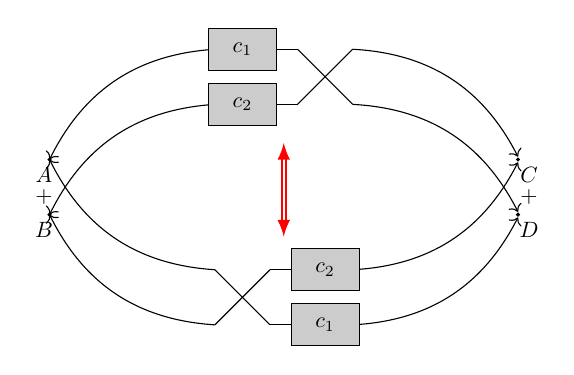
\begin{tikzpicture}[scale=0.7,every node/.style={scale=0.8}]
  \draw[>=latex,<->,double,red,thick] (2.25,-1.2) -- (2.25,-2.9) ;
  \draw[fill] (-2,-1.5) circle [radius=0.025];
  \node[below] at (-2.1,-1.5) {$A$};
  \node[below] at (-2.1,-1.9) {$+$};
  \draw[fill] (-2,-2.5) circle [radius=0.025];
  \node[below] at (-2.1,-2.5) {$B$};

  \draw[fill] (6.5,-1.5) circle [radius=0.025];
  \node[below] at (6.7,-1.5) {$C$};
  \node[below] at (6.7,-1.9) {$+$};
  \draw[fill] (6.5,-2.5) circle [radius=0.025];
  \node[below] at (6.7,-2.5) {$D$};

  \draw[<-] (-2,-1.5) to[bend left] (1,0.5) ;
  \draw[<-] (-2,-2.5) to[bend left] (1,-0.5) ;
  \draw[->] (3.5,0.5) to[bend left] (6.5,-1.45) ;
  \draw[->] (3.5,-0.5) to[bend left] (6.5,-2.45) ;

  \draw[<-] (-2,-1.5) to[bend right] (1,-3.5) ;
  \draw[<-] (-2,-2.5) to[bend right] (1,-4.5) ;
  \draw[->] (3.5,-3.5) to[bend right] (6.5,-1.55) ;
  \draw[->] (3.5,-4.5) to[bend right] (6.5,-2.55) ;


  \draw     (2,0.5)  -- (2.5,0.5)  ;
  \draw     (2,-0.5) -- (2.5,-0.5) ;

  \draw     (2.5,0.5)  -- (3.5,-0.5)  ;
  \draw     (2.5,-0.5) -- (3.5,0.5) ;

  \draw     (1,-3.5)  -- (2,-4.5)    ;
  \draw     (1,-4.5) -- (2,-3.5)   ;

  \draw     (2,-3.5)  -- (2.5,-3.5)    ;
  \draw     (2,-4.5) -- (2.5,-4.5)   ;

  \path (1.5,0.5) node (tc1) [func] {$c_1$};
  \path (1.5,-0.5) node (tc2) [func] {$c_2$};
  \path (3,-4.5) node (bc1) [func] {$c_1$};
  \path (3,-3.5) node (bc2) [func] {$c_2$};
\end{tikzpicture}
\end{center}
The top path is
$(c_1~\oplus~c_2)~\odot~\swapp$ and the bottom path
$\swapp~\odot~(c_2~\oplus~c_1)$. These are equivalent --
and in fact denote the same permutation.
And, of course, not
all programs between the same types are equivalent. The simplest example
are the two automorphisms of $1+1$, namely $\idc$ and $\swapp$.

The language of type isomorphisms and equivalences between
them has a strong connection to \emph{univalent universes} in
HoTT~\cite{Carette2018}. Based on this connection, we refer to the
types as being at level-0, to the equivalences between types as being
at level-1, and to the
equivalences between equivalences of types (i.e., this subsection)
as being at level-2.

The basic type equivalences were defined by using all the
proof terms of commutative semirings. What we need
now is to understand how \emph{proofs} of algebraic identities should be
considered equivalent. Classical algebra does not help, as proofs
are not considered first-class citizens. However,
another route is available to us: since the work of
Hofmann and Streicher~\cite{hofmann96thegroupoid}, we know that
one can model types as \emph{groupoids}.  The additional
structure comes from explicitly modeling the ``identity
types'': instead of regarding all terms which witness
the equality of (say) $a$ and $b$ of type $A$ as being
indistinguishable, we posit that there may in fact be many,
i.e. proof relevance.

Thus, rather than looking at (untyped) commutative semirings, we
should look at a \emph{typed} version. This process frequently goes by
the moniker of ``categorification.''  We want a categorical algebra,
where the basic objects are groupoids (to model our types), and where
there is a natural notion of $+$ and $*$.  At first, we hit what seems
like a serious stumbling block: the category of all groupoids, \Gpd,
have neither co-products nor products. However, we don't want to work
internally in \Gpd -- we want operations \emph{on} groupoids. In other
words, we want something akin to symmetric monoidal categories, but
with two interacting monoidal structures.  Luckily, this already
exists: the categorical analog to (commutative) semirings are
(symmetric) Rig Categories~\cite{laplaza72,kelly74}.  This
straightforwardly generalizes to symmetric Rig Groupoids.

How does this help? Coherence conditions! Symmetric monoidal categories,
to start somewhere simple, do not just introduce natural transformations
like the associator $\alpha$ and the left and right unitors ($\lambda$
and~$\rho$ respectively), but also coherence conditions that these must satisfy.
Looking, for example, at just the additive fragment (i.e. with just $0$,
$1$ and $+$ for the types, $\odot$ and $\oplus$ as combinators, and
only the terms so expressible), the sub-language would correspond,
denotationally, to exactly symmetric monoidal groupoids. And
here we have \emph{equations between equations}, aka
commutative diagrams.  Transporting these coherence conditions, for
example those that express that various transformations are \emph{natural},
to our setting gives a list of equations between isomorphisms.
Furthermore, all the natural transformations
that arise are in fact natural \emph{isomorphisms} -- and thus
reversible.

We can in fact prove that all the coherence conditions
of symmetric Rig Groupoids holds for the groupoid
interpretation of types~\cite{Carette2016}.  This is somewhat tedious
given the sheer numbers involved, but when properly formulated,
relatively straightforward, up to a couple of tricky cases.

But why are these particular coherence laws? Are they all necessary?
Conversely are they, in some appropriate sense, sufficient? This is
the so-called \emph{coherence problem}. Mac Lane, in his farewell address
as President of the American Mathematical Society~\cite{MacLane1976} gives
a good introduction and overview of such problems.  A more modern
interpretation (which can nevertheless be read into Mac Lane's own
exposition) would read as follows: given a set of equalities on abstract
words, regarded as a rewrite system, and two means of rewriting a word
in that language to another, is there some suitable notion of canonical
form that expresses the essential uniqueness of the non-trivial
rewrites?  Note how this word-and-rewrite problem is essentially
independent of the eventual interpretation. But one must take some care,
as there are obvious degenerate cases (involving ``trivial'' equations
involving $0$ or $1$) which lead to non-uniqueness. The landmark
results, first by Kelly-Mac Lane~\cite{KELLY197197} for closed
symmetric monoidal categories, then (independently) Laplaza and
Kelly~\cite{laplaza72,kelly74} for symmetric Rig Categories, is
that indeed there are sound and complete coherence conditions that
insure that all the ``obvious'' equalities between different abstract
words in these systems give rise to commutative diagrams. The
``obvious'' equalities come from \emph{syzygies} or
\emph{critical pairs} of the system of equations.
The problem is far from trivial --- Fiore et al.~\cite{Fiore-2008}
document some publications where the coherence set is in
fact incorrect. They furthermore give a quite general algorithm
to derive such coherence conditions.

\section{Exploring the Lens landscape}

Given that we have a sound and complete set of primitive type equivalences
(and combinators),
we can explore what this means for actually programming lenses. Many papers
have explored the most general settings for lenses, we will instead look
inside the implementations.  This will
reveal the \emph{inner structure} of lenses, rather than focusing on their
macro structure.

\subsection{Simple Lenses}
Let's explore the simplest lenses first.  For a \AgdaRecord{GS-Lens}, the simplest is
when \AgdaField{get} is the identity, which forces the rest:

\begin{code}%
\>[0]\AgdaKeyword{module}\AgdaSpace{}%
\AgdaModule{\AgdaUnderscore{}}\AgdaSpace{}%
\AgdaSymbol{(}\AgdaBound{A}\AgdaSpace{}%
\AgdaBound{B}\AgdaSpace{}%
\AgdaBound{D}\AgdaSpace{}%
\AgdaBound{E}\AgdaSpace{}%
\AgdaSymbol{:}\AgdaSpace{}%
\AgdaPrimitiveType{Set}\AgdaSymbol{)}\AgdaSpace{}%
\AgdaKeyword{where}\<%
\\
\>[0][@{}l@{\AgdaIndent{0}}]%
\>[2]\AgdaKeyword{open}\AgdaSpace{}%
\AgdaModule{∃{-}Lens}\<%
\\
%
\\[\AgdaEmptyExtraSkip]%
%
\>[2]\AgdaFunction{AA{-}gs{-}lens}\AgdaSpace{}%
\AgdaSymbol{:}\AgdaSpace{}%
\AgdaRecord{GS{-}Lens}\AgdaSpace{}%
\AgdaBound{A}\AgdaSpace{}%
\AgdaBound{A}\<%
\\
%
\>[2]\AgdaFunction{AA{-}gs{-}lens}\AgdaSpace{}%
\AgdaSymbol{=}\AgdaSpace{}%
\AgdaKeyword{record}\AgdaSpace{}%
\AgdaSymbol{\{}\AgdaSpace{}%
\AgdaField{get}\AgdaSpace{}%
\AgdaSymbol{=}\AgdaSpace{}%
\AgdaFunction{id}\AgdaSpace{}%
\AgdaSymbol{;}\AgdaSpace{}%
\AgdaField{set}\AgdaSpace{}%
\AgdaSymbol{=}\AgdaSpace{}%
\AgdaSymbol{λ}\AgdaSpace{}%
\AgdaBound{\AgdaUnderscore{}}\AgdaSpace{}%
\AgdaSymbol{→}\AgdaSpace{}%
\AgdaFunction{id}\<%
\\
\>[2][@{}l@{\AgdaIndent{0}}]%
\>[4]\AgdaSymbol{;}\AgdaSpace{}%
\AgdaField{getput}\AgdaSpace{}%
\AgdaSymbol{=}\AgdaSpace{}%
\AgdaSymbol{λ}\AgdaSpace{}%
\AgdaBound{\AgdaUnderscore{}}\AgdaSpace{}%
\AgdaBound{\AgdaUnderscore{}}\AgdaSpace{}%
\AgdaSymbol{→}\AgdaSpace{}%
\AgdaInductiveConstructor{P.refl}\AgdaSpace{}%
\AgdaSymbol{;}\AgdaSpace{}%
\AgdaField{putget}\AgdaSpace{}%
\AgdaSymbol{=}\AgdaSpace{}%
\AgdaSymbol{λ}\AgdaSpace{}%
\AgdaBound{\AgdaUnderscore{}}\AgdaSpace{}%
\AgdaSymbol{→}\AgdaSpace{}%
\AgdaInductiveConstructor{P.refl}\AgdaSpace{}%
\AgdaSymbol{;}\AgdaSpace{}%
\AgdaField{putput}\AgdaSpace{}%
\AgdaSymbol{=}\AgdaSpace{}%
\AgdaSymbol{λ}\AgdaSpace{}%
\AgdaBound{\AgdaUnderscore{}}\AgdaSpace{}%
\AgdaBound{\AgdaUnderscore{}}\AgdaSpace{}%
\AgdaBound{\AgdaUnderscore{}}\AgdaSpace{}%
\AgdaSymbol{→}\AgdaSpace{}%
\AgdaInductiveConstructor{P.refl}\AgdaSpace{}%
\AgdaSymbol{\}}\<%
\end{code}

What does that correspond to as a \AgdaRecord{∃-Lens}? Here, we can easily
guess the complement by solving the equation $A ≃ C × A$ for $C$: $C$ must
be $\AgdaSymbol{⊤}$. But then the $\AgdaRecord{∃-Lens}$ isn't quite as simple as above:
\begin{code}%
%
\>[2]\AgdaFunction{AA{-}∃{-}lens}\AgdaSpace{}%
\AgdaSymbol{:}\AgdaSpace{}%
\AgdaRecord{∃{-}Lens}\AgdaSpace{}%
\AgdaBound{A}\AgdaSpace{}%
\AgdaBound{A}\<%
\\
%
\>[2]\AgdaFunction{AA{-}∃{-}lens}\AgdaSpace{}%
\AgdaSymbol{=}\AgdaSpace{}%
\AgdaFunction{lens}\AgdaSpace{}%
\AgdaFunction{uniti⋆equiv}\<%
\end{code}
\noindent where $\AgdaFunction{uniti⋆equiv}$ has type
$A ≃ (⊤ × A)$. In other words, as the complement is not actually
present in $A$, it must be introduced. $\AgdaFunction{uniti⋆equiv}$
names the ``multiplicative unit introduction equivalence''. From
here on, we will not expand on the names, trusting that they
can be guessed by the reader.

What about in the other direction, what is the \AgdaRecord{∃-Lens} whose
underlying isomorphism is the identity?
\begin{code}%
%
\>[2]\AgdaFunction{BAA{-}∃{-}lens}\AgdaSpace{}%
\AgdaSymbol{:}\AgdaSpace{}%
\AgdaRecord{∃{-}Lens}\AgdaSpace{}%
\AgdaSymbol{(}\AgdaBound{B}\AgdaSpace{}%
\AgdaOperator{\AgdaFunction{×}}\AgdaSpace{}%
\AgdaBound{A}\AgdaSymbol{)}\AgdaSpace{}%
\AgdaBound{A}\<%
\\
%
\>[2]\AgdaFunction{BAA{-}∃{-}lens}\AgdaSpace{}%
\AgdaSymbol{=}\AgdaSpace{}%
\AgdaFunction{lens}\AgdaSpace{}%
\AgdaFunction{id≃}\<%
\end{code}
\noindent Since our definition of \AgdaRecord{∃-Lens} is right-biased
(we are looking for isomorphisms of shape $S ≃ C × A$), the above lens
extracts the $A$ on the right.  Of course, there is another lens which
switches the roles of $A$ and $B$ --- and this leaves a trace on the
isomorphism:
\begin{code}%
%
\>[2]\AgdaFunction{BAB{-}∃{-}lens}\AgdaSpace{}%
\AgdaSymbol{:}\AgdaSpace{}%
\AgdaRecord{∃{-}Lens}\AgdaSpace{}%
\AgdaSymbol{(}\AgdaBound{B}\AgdaSpace{}%
\AgdaOperator{\AgdaFunction{×}}\AgdaSpace{}%
\AgdaBound{A}\AgdaSymbol{)}\AgdaSpace{}%
\AgdaBound{B}\<%
\\
%
\>[2]\AgdaFunction{BAB{-}∃{-}lens}\AgdaSpace{}%
\AgdaSymbol{=}\AgdaSpace{}%
\AgdaFunction{lens}\AgdaSpace{}%
\AgdaFunction{swap⋆equiv}\<%
\end{code}

Thus, looking at type equivalences, which ones return a type
of shape $C × A$ ?  We have already seen \AIC{uniti⋆l},
\AIC{id⟷} and \AIC{swap⋆} arise. That leaves four:
\AIC{assocl⋆}, \AIC{factorz}, \AIC{factor} and \AIC{×≃}.
These occur as follows:
\begin{code}%
%
\>[2]\AgdaFunction{DBA{-}lens}\AgdaSpace{}%
\AgdaSymbol{:}\AgdaSpace{}%
\AgdaRecord{∃{-}Lens}\AgdaSpace{}%
\AgdaSymbol{(}\AgdaBound{D}\AgdaSpace{}%
\AgdaOperator{\AgdaFunction{×}}\AgdaSpace{}%
\AgdaSymbol{(}\AgdaBound{B}\AgdaSpace{}%
\AgdaOperator{\AgdaFunction{×}}\AgdaSpace{}%
\AgdaBound{A}\AgdaSymbol{))}\AgdaSpace{}%
\AgdaBound{A}\<%
\\
%
\>[2]\AgdaFunction{DBA{-}lens}\AgdaSpace{}%
\AgdaSymbol{=}\AgdaSpace{}%
\AgdaFunction{lens}\AgdaSpace{}%
\AgdaFunction{assocl⋆equiv}\<%
\\
%
\\[\AgdaEmptyExtraSkip]%
%
\>[2]\AgdaFunction{⊥{-}lens}\AgdaSpace{}%
\AgdaSymbol{:}\AgdaSpace{}%
\AgdaRecord{∃{-}Lens}\AgdaSpace{}%
\AgdaDatatype{⊥}\AgdaSpace{}%
\AgdaBound{A}\<%
\\
%
\>[2]\AgdaFunction{⊥{-}lens}\AgdaSpace{}%
\AgdaSymbol{=}\AgdaSpace{}%
\AgdaFunction{lens}\AgdaSpace{}%
\AgdaFunction{factorzequiv}\<%
\\
%
\\[\AgdaEmptyExtraSkip]%
%
\>[2]\AgdaFunction{⊎{-}lens}\AgdaSpace{}%
\AgdaSymbol{:}\AgdaSpace{}%
\AgdaRecord{∃{-}Lens}\AgdaSpace{}%
\AgdaSymbol{((}\AgdaBound{D}\AgdaSpace{}%
\AgdaOperator{\AgdaFunction{×}}\AgdaSpace{}%
\AgdaBound{A}\AgdaSymbol{)}\AgdaSpace{}%
\AgdaOperator{\AgdaDatatype{⊎}}\AgdaSpace{}%
\AgdaSymbol{(}\AgdaBound{B}\AgdaSpace{}%
\AgdaOperator{\AgdaFunction{×}}\AgdaSpace{}%
\AgdaBound{A}\AgdaSymbol{))}\AgdaSpace{}%
\AgdaBound{A}\<%
\\
%
\>[2]\AgdaFunction{⊎{-}lens}\AgdaSpace{}%
\AgdaSymbol{=}\AgdaSpace{}%
\AgdaFunction{lens}\AgdaSpace{}%
\AgdaFunction{factorequiv}\<%
\\
%
\\[\AgdaEmptyExtraSkip]%
%
\>[2]\AgdaFunction{⊗{-}lens}\AgdaSpace{}%
\AgdaSymbol{:}\AgdaSpace{}%
\AgdaSymbol{(}\AgdaBound{E}\AgdaSpace{}%
\AgdaOperator{\AgdaFunction{≃}}\AgdaSpace{}%
\AgdaBound{B}\AgdaSymbol{)}\AgdaSpace{}%
\AgdaSymbol{→}\AgdaSpace{}%
\AgdaSymbol{(}\AgdaBound{D}\AgdaSpace{}%
\AgdaOperator{\AgdaFunction{≃}}\AgdaSpace{}%
\AgdaBound{A}\AgdaSymbol{)}\AgdaSpace{}%
\AgdaSymbol{→}\AgdaSpace{}%
\AgdaRecord{∃{-}Lens}\AgdaSpace{}%
\AgdaSymbol{(}\AgdaBound{E}\AgdaSpace{}%
\AgdaOperator{\AgdaFunction{×}}\AgdaSpace{}%
\AgdaBound{D}\AgdaSymbol{)}\AgdaSpace{}%
\AgdaBound{A}\<%
\\
%
\>[2]\AgdaFunction{⊗{-}lens}\AgdaSpace{}%
\AgdaBound{iso₁}\AgdaSpace{}%
\AgdaBound{iso₂}\AgdaSpace{}%
\AgdaSymbol{=}\AgdaSpace{}%
\AgdaFunction{lens}\AgdaSpace{}%
\AgdaSymbol{(}\AgdaBound{iso₁}\AgdaSpace{}%
\AgdaOperator{\AgdaFunction{×≃}}\AgdaSpace{}%
\AgdaBound{iso₂}\AgdaSymbol{)}\<%
\end{code}

The first is a basic administrative ``reshaping''. The second
takes a bit more thought, but is easily explained: if we promise
an impossible source, it is easy to promise to return something
arbitrary in return!

The $\AgdaFunction{⊎-lens}$ is interesting, because it allows us
to see a constant complement in a type which itself is not a
product -- it is, however, equivalent to one. The last uses the
full power of equivalences, to see an $A$ where, a priori, one
does not seem to exist at all.

Lastly, we also have lens composition:
\begin{code}%
%
\>[2]\AgdaFunction{∘{-}lens}\AgdaSpace{}%
\AgdaSymbol{:}\AgdaSpace{}%
\AgdaRecord{∃{-}Lens}\AgdaSpace{}%
\AgdaBound{D}\AgdaSpace{}%
\AgdaBound{B}\AgdaSpace{}%
\AgdaSymbol{→}\AgdaSpace{}%
\AgdaRecord{∃{-}Lens}\AgdaSpace{}%
\AgdaBound{B}\AgdaSpace{}%
\AgdaBound{A}\AgdaSpace{}%
\AgdaSymbol{→}\AgdaSpace{}%
\AgdaRecord{∃{-}Lens}\AgdaSpace{}%
\AgdaBound{D}\AgdaSpace{}%
\AgdaBound{A}\<%
\\
%
\>[2]\AgdaFunction{∘{-}lens}\AgdaSpace{}%
\AgdaBound{l₁}\AgdaSpace{}%
\AgdaBound{l₂}\AgdaSpace{}%
\AgdaSymbol{=}\AgdaSpace{}%
\AgdaInductiveConstructor{ll}\AgdaSpace{}%
\AgdaSymbol{((}\AgdaFunction{×{-}assoc}\AgdaSpace{}%
\AgdaOperator{\AgdaFunction{∘F}}\AgdaSpace{}%
\AgdaSymbol{(}\AgdaFunction{idF}\AgdaSpace{}%
\AgdaOperator{\AgdaFunction{×{-}inverse}}\AgdaSpace{}%
\AgdaField{∃{-}Lens.iso}\AgdaSpace{}%
\AgdaBound{l₂}\AgdaSymbol{))}\AgdaSpace{}%
\AgdaOperator{\AgdaFunction{∘F}}\AgdaSpace{}%
\AgdaField{∃{-}Lens.iso}\AgdaSpace{}%
\AgdaBound{l₁}\AgdaSymbol{)}\<%
\end{code}
The above gives us our first \emph{lens program} consisting of a composition of
four more basic equivalences. However, it is ``lower level'' as we can only
extract $\AgdaRecord{Setoid}$-based equivalences from a $\AgdaRecord{∃-Lens}$.
The necessary code is quite straightforward (and available in the literate
Agda source of this paper).

\subsection{Unusual lenses}

It is possible to create lenses for things which are
not ``in'' a type at all --- an example is most instructive.
For completeness, both \AgdaRecord{GS-Lens} and \AgdaRecord{∃-Lens}
will be given.

Let us consider a type \verb|Colour| with exactly $3$ inhabitants,
\begin{code}%
\>[0]\AgdaKeyword{module}\AgdaSpace{}%
\AgdaModule{\AgdaUnderscore{}}\AgdaSpace{}%
\AgdaSymbol{\{}\AgdaBound{A}\AgdaSpace{}%
\AgdaSymbol{:}\AgdaSpace{}%
\AgdaPrimitiveType{Set}\AgdaSymbol{\}}\AgdaSpace{}%
\AgdaKeyword{where}\<%
\\
\>[0][@{}l@{\AgdaIndent{0}}]%
\>[2]\AgdaKeyword{data}\AgdaSpace{}%
\AgdaDatatype{Colour}\AgdaSpace{}%
\AgdaSymbol{:}\AgdaSpace{}%
\AgdaPrimitiveType{Set}\AgdaSpace{}%
\AgdaKeyword{where}\AgdaSpace{}%
\AgdaInductiveConstructor{red}\AgdaSpace{}%
\AgdaInductiveConstructor{green}\AgdaSpace{}%
\AgdaInductiveConstructor{blue}\AgdaSpace{}%
\AgdaSymbol{:}\AgdaSpace{}%
\AgdaDatatype{Colour}\<%
\end{code}

First, a \AgdaRecord{∃-Lens} built ``by hand'':
\begin{code}%
%
\>[2]\AgdaFunction{∃{-}Colour{-}in{-}A+A+A}\AgdaSpace{}%
\AgdaSymbol{:}\AgdaSpace{}%
\AgdaRecord{∃{-}Lens}\AgdaSpace{}%
\AgdaSymbol{(}\AgdaBound{A}\AgdaSpace{}%
\AgdaOperator{\AgdaDatatype{⊎}}\AgdaSpace{}%
\AgdaBound{A}\AgdaSpace{}%
\AgdaOperator{\AgdaDatatype{⊎}}\AgdaSpace{}%
\AgdaBound{A}\AgdaSymbol{)}\AgdaSpace{}%
\AgdaDatatype{Colour}\<%
\\
%
\>[2]\AgdaFunction{∃{-}Colour{-}in{-}A+A+A}\AgdaSpace{}%
\AgdaSymbol{=}\AgdaSpace{}%
\AgdaFunction{lens}\AgdaSpace{}%
\AgdaFunction{equ}\<%
\\
\>[2][@{}l@{\AgdaIndent{0}}]%
\>[3]\AgdaKeyword{where}\<%
\\
\>[3][@{}l@{\AgdaIndent{0}}]%
\>[4]\AgdaFunction{f}\AgdaSpace{}%
\AgdaSymbol{:}\AgdaSpace{}%
\AgdaBound{A}\AgdaSpace{}%
\AgdaOperator{\AgdaDatatype{⊎}}\AgdaSpace{}%
\AgdaBound{A}\AgdaSpace{}%
\AgdaOperator{\AgdaDatatype{⊎}}\AgdaSpace{}%
\AgdaBound{A}\AgdaSpace{}%
\AgdaSymbol{→}\AgdaSpace{}%
\AgdaBound{A}\AgdaSpace{}%
\AgdaOperator{\AgdaFunction{×}}\AgdaSpace{}%
\AgdaDatatype{Colour}\<%
\\
%
\>[4]\AgdaFunction{f}\AgdaSpace{}%
\AgdaSymbol{(}\AgdaInductiveConstructor{inj₁}\AgdaSpace{}%
\AgdaBound{x}\AgdaSymbol{)}\AgdaSpace{}%
\AgdaSymbol{=}\AgdaSpace{}%
\AgdaBound{x}\AgdaSpace{}%
\AgdaOperator{\AgdaInductiveConstructor{,}}\AgdaSpace{}%
\AgdaInductiveConstructor{red}\<%
\\
%
\>[4]\AgdaFunction{f}\AgdaSpace{}%
\AgdaSymbol{(}\AgdaInductiveConstructor{inj₂}\AgdaSpace{}%
\AgdaSymbol{(}\AgdaInductiveConstructor{inj₁}\AgdaSpace{}%
\AgdaBound{x}\AgdaSymbol{))}\AgdaSpace{}%
\AgdaSymbol{=}\AgdaSpace{}%
\AgdaBound{x}\AgdaSpace{}%
\AgdaOperator{\AgdaInductiveConstructor{,}}\AgdaSpace{}%
\AgdaInductiveConstructor{green}\<%
\\
%
\>[4]\AgdaFunction{f}\AgdaSpace{}%
\AgdaSymbol{(}\AgdaInductiveConstructor{inj₂}\AgdaSpace{}%
\AgdaSymbol{(}\AgdaInductiveConstructor{inj₂}\AgdaSpace{}%
\AgdaBound{x}\AgdaSymbol{))}\AgdaSpace{}%
\AgdaSymbol{=}\AgdaSpace{}%
\AgdaBound{x}\AgdaSpace{}%
\AgdaOperator{\AgdaInductiveConstructor{,}}\AgdaSpace{}%
\AgdaInductiveConstructor{blue}\<%
\\
%
\>[4]\AgdaFunction{g}\AgdaSpace{}%
\AgdaSymbol{:}\AgdaSpace{}%
\AgdaBound{A}\AgdaSpace{}%
\AgdaOperator{\AgdaFunction{×}}\AgdaSpace{}%
\AgdaDatatype{Colour}\AgdaSpace{}%
\AgdaSymbol{→}\AgdaSpace{}%
\AgdaBound{A}\AgdaSpace{}%
\AgdaOperator{\AgdaDatatype{⊎}}\AgdaSpace{}%
\AgdaBound{A}\AgdaSpace{}%
\AgdaOperator{\AgdaDatatype{⊎}}\AgdaSpace{}%
\AgdaBound{A}\<%
\\
%
\>[4]\AgdaFunction{g}\AgdaSpace{}%
\AgdaSymbol{(}\AgdaBound{a}\AgdaSpace{}%
\AgdaOperator{\AgdaInductiveConstructor{,}}\AgdaSpace{}%
\AgdaInductiveConstructor{red}\AgdaSymbol{)}\AgdaSpace{}%
\AgdaSymbol{=}\AgdaSpace{}%
\AgdaInductiveConstructor{inj₁}\AgdaSpace{}%
\AgdaBound{a}\<%
\\
%
\>[4]\AgdaFunction{g}\AgdaSpace{}%
\AgdaSymbol{(}\AgdaBound{a}\AgdaSpace{}%
\AgdaOperator{\AgdaInductiveConstructor{,}}\AgdaSpace{}%
\AgdaInductiveConstructor{green}\AgdaSymbol{)}\AgdaSpace{}%
\AgdaSymbol{=}\AgdaSpace{}%
\AgdaInductiveConstructor{inj₂}\AgdaSpace{}%
\AgdaSymbol{(}\AgdaInductiveConstructor{inj₁}\AgdaSpace{}%
\AgdaBound{a}\AgdaSymbol{)}\<%
\\
%
\>[4]\AgdaFunction{g}\AgdaSpace{}%
\AgdaSymbol{(}\AgdaBound{a}\AgdaSpace{}%
\AgdaOperator{\AgdaInductiveConstructor{,}}\AgdaSpace{}%
\AgdaInductiveConstructor{blue}\AgdaSymbol{)}\AgdaSpace{}%
\AgdaSymbol{=}\AgdaSpace{}%
\AgdaInductiveConstructor{inj₂}\AgdaSpace{}%
\AgdaSymbol{(}\AgdaInductiveConstructor{inj₂}\AgdaSpace{}%
\AgdaBound{a}\AgdaSymbol{)}\<%
\\
%
\>[4]\AgdaFunction{equ}\AgdaSpace{}%
\AgdaSymbol{:}\AgdaSpace{}%
\AgdaSymbol{(}\AgdaBound{A}\AgdaSpace{}%
\AgdaOperator{\AgdaDatatype{⊎}}\AgdaSpace{}%
\AgdaBound{A}\AgdaSpace{}%
\AgdaOperator{\AgdaDatatype{⊎}}\AgdaSpace{}%
\AgdaBound{A}\AgdaSymbol{)}\AgdaSpace{}%
\AgdaOperator{\AgdaFunction{≃}}\AgdaSpace{}%
\AgdaSymbol{(}\AgdaBound{A}\AgdaSpace{}%
\AgdaOperator{\AgdaFunction{×}}\AgdaSpace{}%
\AgdaDatatype{Colour}\AgdaSymbol{)}\<%
\\
%
\>[4]\AgdaFunction{equ}\AgdaSpace{}%
\AgdaSymbol{=}\AgdaSpace{}%
\AgdaFunction{f}\AgdaSpace{}%
\AgdaOperator{\AgdaInductiveConstructor{,}}\AgdaSpace{}%
\AgdaInductiveConstructor{qinv}\AgdaSpace{}%
\AgdaFunction{g}%
\>[1612I]\AgdaSymbol{(λ}\AgdaSpace{}%
\AgdaSymbol{\{}\AgdaSpace{}%
\AgdaSymbol{(}\AgdaBound{a}\AgdaSpace{}%
\AgdaOperator{\AgdaInductiveConstructor{,}}\AgdaSpace{}%
\AgdaInductiveConstructor{red}\AgdaSymbol{)}\AgdaSpace{}%
\AgdaSymbol{→}\AgdaSpace{}%
\AgdaInductiveConstructor{refl}\AgdaSpace{}%
\AgdaSymbol{;}\AgdaSpace{}%
\AgdaSymbol{(}\AgdaBound{a}\AgdaSpace{}%
\AgdaOperator{\AgdaInductiveConstructor{,}}\AgdaSpace{}%
\AgdaInductiveConstructor{green}\AgdaSymbol{)}\AgdaSpace{}%
\AgdaSymbol{→}\AgdaSpace{}%
\AgdaInductiveConstructor{refl}\AgdaSpace{}%
\AgdaSymbol{;}\AgdaSpace{}%
\AgdaSymbol{(}\AgdaBound{a}\AgdaSpace{}%
\AgdaOperator{\AgdaInductiveConstructor{,}}\AgdaSpace{}%
\AgdaInductiveConstructor{blue}\AgdaSymbol{)}\AgdaSpace{}%
\AgdaSymbol{→}\AgdaSpace{}%
\AgdaInductiveConstructor{refl}\AgdaSymbol{\})}\<%
\\
\>[.]\<[1612I]%
\>[21]\AgdaSymbol{λ}\AgdaSpace{}%
\AgdaSymbol{\{}\AgdaSpace{}%
\AgdaSymbol{(}\AgdaInductiveConstructor{inj₁}\AgdaSpace{}%
\AgdaBound{x}\AgdaSymbol{)}\AgdaSpace{}%
\AgdaSymbol{→}\AgdaSpace{}%
\AgdaInductiveConstructor{refl}\AgdaSpace{}%
\AgdaSymbol{;}\AgdaSpace{}%
\AgdaSymbol{(}\AgdaInductiveConstructor{inj₂}\AgdaSpace{}%
\AgdaSymbol{(}\AgdaInductiveConstructor{inj₁}\AgdaSpace{}%
\AgdaBound{x}\AgdaSymbol{))}\AgdaSpace{}%
\AgdaSymbol{→}\AgdaSpace{}%
\AgdaInductiveConstructor{refl}\AgdaSpace{}%
\AgdaSymbol{;}\AgdaSpace{}%
\AgdaSymbol{(}\AgdaInductiveConstructor{inj₂}\AgdaSpace{}%
\AgdaSymbol{(}\AgdaInductiveConstructor{inj₂}\AgdaSpace{}%
\AgdaBound{y}\AgdaSymbol{))}\AgdaSpace{}%
\AgdaSymbol{→}\AgdaSpace{}%
\AgdaInductiveConstructor{refl}\AgdaSymbol{\}}\<%
\end{code}
The equivalence is not too painful to establish. But let's do
the same for the \verb|GS-Lens|:
\begin{code}%
%
\>[2]\AgdaFunction{GS{-}Colour{-}in{-}A+A+A}\AgdaSpace{}%
\AgdaSymbol{:}\AgdaSpace{}%
\AgdaRecord{GS{-}Lens}\AgdaSpace{}%
\AgdaSymbol{(}\AgdaBound{A}\AgdaSpace{}%
\AgdaOperator{\AgdaDatatype{⊎}}\AgdaSpace{}%
\AgdaBound{A}\AgdaSpace{}%
\AgdaOperator{\AgdaDatatype{⊎}}\AgdaSpace{}%
\AgdaBound{A}\AgdaSymbol{)}\AgdaSpace{}%
\AgdaDatatype{Colour}\<%
\\
%
\>[2]\AgdaFunction{GS{-}Colour{-}in{-}A+A+A}\AgdaSpace{}%
\AgdaSymbol{=}\AgdaSpace{}%
\AgdaKeyword{record}\<%
\\
\>[2][@{}l@{\AgdaIndent{0}}]%
\>[4]\AgdaSymbol{\{}\AgdaSpace{}%
\AgdaField{get}\AgdaSpace{}%
\AgdaSymbol{=}\AgdaSpace{}%
\AgdaSymbol{λ}\AgdaSpace{}%
\AgdaSymbol{\{}\AgdaSpace{}%
\AgdaSymbol{(}\AgdaInductiveConstructor{inj₁}\AgdaSpace{}%
\AgdaBound{x}\AgdaSymbol{)}\AgdaSpace{}%
\AgdaSymbol{→}\AgdaSpace{}%
\AgdaInductiveConstructor{red}\AgdaSpace{}%
\AgdaSymbol{;}\AgdaSpace{}%
\AgdaSymbol{(}\AgdaInductiveConstructor{inj₂}\AgdaSpace{}%
\AgdaSymbol{(}\AgdaInductiveConstructor{inj₁}\AgdaSpace{}%
\AgdaBound{x}\AgdaSymbol{))}\AgdaSpace{}%
\AgdaSymbol{→}\AgdaSpace{}%
\AgdaInductiveConstructor{green}\AgdaSpace{}%
\AgdaSymbol{;}\AgdaSpace{}%
\AgdaSymbol{(}\AgdaInductiveConstructor{inj₂}\AgdaSpace{}%
\AgdaSymbol{(}\AgdaInductiveConstructor{inj₂}\AgdaSpace{}%
\AgdaBound{y}\AgdaSymbol{))}\AgdaSpace{}%
\AgdaSymbol{→}\AgdaSpace{}%
\AgdaInductiveConstructor{blue}\AgdaSymbol{\}}\<%
\\
%
\>[4]\AgdaSymbol{;}\AgdaSpace{}%
\AgdaField{set}\AgdaSpace{}%
\AgdaSymbol{=}\AgdaSpace{}%
\AgdaSymbol{λ}%
\>[1681I]\AgdaSymbol{\{}\AgdaSpace{}%
\AgdaSymbol{(}\AgdaInductiveConstructor{inj₁}\AgdaSpace{}%
\AgdaBound{x}\AgdaSymbol{)}\AgdaSpace{}%
\AgdaInductiveConstructor{red}\AgdaSpace{}%
\AgdaSymbol{→}\AgdaSpace{}%
\AgdaInductiveConstructor{inj₁}\AgdaSpace{}%
\AgdaBound{x}\AgdaSpace{}%
\AgdaSymbol{;}\AgdaSpace{}%
\AgdaSymbol{(}\AgdaInductiveConstructor{inj₁}\AgdaSpace{}%
\AgdaBound{x}\AgdaSymbol{)}\AgdaSpace{}%
\AgdaInductiveConstructor{green}\AgdaSpace{}%
\AgdaSymbol{→}\AgdaSpace{}%
\AgdaInductiveConstructor{inj₂}\AgdaSpace{}%
\AgdaSymbol{(}\AgdaInductiveConstructor{inj₁}\AgdaSpace{}%
\AgdaBound{x}\AgdaSymbol{)}\AgdaSpace{}%
\AgdaSymbol{;}\AgdaSpace{}%
\AgdaSymbol{(}\AgdaInductiveConstructor{inj₁}\AgdaSpace{}%
\AgdaBound{x}\AgdaSymbol{)}\AgdaSpace{}%
\AgdaInductiveConstructor{blue}\AgdaSpace{}%
\AgdaSymbol{→}\AgdaSpace{}%
\AgdaInductiveConstructor{inj₂}\AgdaSpace{}%
\AgdaSymbol{(}\AgdaInductiveConstructor{inj₂}\AgdaSpace{}%
\AgdaBound{x}\AgdaSymbol{)}\<%
\\
\>[.]\<[1681I]%
\>[14]\AgdaSymbol{;}\AgdaSpace{}%
\AgdaSymbol{(}\AgdaInductiveConstructor{inj₂}\AgdaSpace{}%
\AgdaSymbol{(}\AgdaInductiveConstructor{inj₁}\AgdaSpace{}%
\AgdaBound{x}\AgdaSymbol{))}\AgdaSpace{}%
\AgdaInductiveConstructor{red}\AgdaSpace{}%
\AgdaSymbol{→}\AgdaSpace{}%
\AgdaInductiveConstructor{inj₁}\AgdaSpace{}%
\AgdaBound{x}\AgdaSpace{}%
\AgdaSymbol{;}\AgdaSpace{}%
\AgdaSymbol{(}\AgdaInductiveConstructor{inj₂}\AgdaSpace{}%
\AgdaSymbol{(}\AgdaInductiveConstructor{inj₁}\AgdaSpace{}%
\AgdaBound{x}\AgdaSymbol{))}\AgdaSpace{}%
\AgdaInductiveConstructor{green}\AgdaSpace{}%
\AgdaSymbol{→}\AgdaSpace{}%
\AgdaInductiveConstructor{inj₂}\AgdaSpace{}%
\AgdaSymbol{(}\AgdaInductiveConstructor{inj₁}\AgdaSpace{}%
\AgdaBound{x}\AgdaSymbol{)}\AgdaSpace{}%
\AgdaSymbol{;}\AgdaSpace{}%
\AgdaSymbol{(}\AgdaInductiveConstructor{inj₂}\AgdaSpace{}%
\AgdaSymbol{(}\AgdaInductiveConstructor{inj₁}\AgdaSpace{}%
\AgdaBound{x}\AgdaSymbol{))}\AgdaSpace{}%
\AgdaInductiveConstructor{blue}\AgdaSpace{}%
\AgdaSymbol{→}\AgdaSpace{}%
\AgdaInductiveConstructor{inj₂}\AgdaSpace{}%
\AgdaSymbol{(}\AgdaInductiveConstructor{inj₂}\AgdaSpace{}%
\AgdaBound{x}\AgdaSymbol{)}\<%
\\
%
\>[14]\AgdaSymbol{;}\AgdaSpace{}%
\AgdaSymbol{(}\AgdaInductiveConstructor{inj₂}\AgdaSpace{}%
\AgdaSymbol{(}\AgdaInductiveConstructor{inj₂}\AgdaSpace{}%
\AgdaBound{y}\AgdaSymbol{))}\AgdaSpace{}%
\AgdaInductiveConstructor{red}\AgdaSpace{}%
\AgdaSymbol{→}\AgdaSpace{}%
\AgdaInductiveConstructor{inj₁}\AgdaSpace{}%
\AgdaBound{y}\AgdaSpace{}%
\AgdaSymbol{;}\AgdaSpace{}%
\AgdaSymbol{(}\AgdaInductiveConstructor{inj₂}\AgdaSpace{}%
\AgdaSymbol{(}\AgdaInductiveConstructor{inj₂}\AgdaSpace{}%
\AgdaBound{y}\AgdaSymbol{))}\AgdaSpace{}%
\AgdaInductiveConstructor{green}\AgdaSpace{}%
\AgdaSymbol{→}\AgdaSpace{}%
\AgdaInductiveConstructor{inj₂}\AgdaSpace{}%
\AgdaSymbol{(}\AgdaInductiveConstructor{inj₁}\AgdaSpace{}%
\AgdaBound{y}\AgdaSymbol{)}\AgdaSpace{}%
\AgdaSymbol{;}\AgdaSpace{}%
\AgdaSymbol{(}\AgdaInductiveConstructor{inj₂}\AgdaSpace{}%
\AgdaSymbol{(}\AgdaInductiveConstructor{inj₂}\AgdaSpace{}%
\AgdaBound{y}\AgdaSymbol{))}\AgdaSpace{}%
\AgdaInductiveConstructor{blue}\AgdaSpace{}%
\AgdaSymbol{→}\AgdaSpace{}%
\AgdaInductiveConstructor{inj₂}\AgdaSpace{}%
\AgdaSymbol{(}\AgdaInductiveConstructor{inj₂}\AgdaSpace{}%
\AgdaBound{y}\AgdaSymbol{)\}}\<%
\\
%
\>[4]\AgdaSymbol{;}\AgdaSpace{}%
\AgdaField{getput}\AgdaSpace{}%
\AgdaSymbol{=}\AgdaSpace{}%
\AgdaSymbol{λ}%
\>[1757I]\AgdaSymbol{\{}\AgdaSpace{}%
\AgdaSymbol{(}\AgdaInductiveConstructor{inj₁}\AgdaSpace{}%
\AgdaBound{x}\AgdaSymbol{)}\AgdaSpace{}%
\AgdaInductiveConstructor{red}\AgdaSpace{}%
\AgdaSymbol{→}\AgdaSpace{}%
\AgdaInductiveConstructor{refl}\AgdaSpace{}%
\AgdaSymbol{;}\AgdaSpace{}%
\AgdaSymbol{(}\AgdaInductiveConstructor{inj₁}\AgdaSpace{}%
\AgdaBound{x}\AgdaSymbol{)}\AgdaSpace{}%
\AgdaInductiveConstructor{green}\AgdaSpace{}%
\AgdaSymbol{→}\AgdaSpace{}%
\AgdaInductiveConstructor{refl}\AgdaSpace{}%
\AgdaSymbol{;}\AgdaSpace{}%
\AgdaSymbol{(}\AgdaInductiveConstructor{inj₁}\AgdaSpace{}%
\AgdaBound{x}\AgdaSymbol{)}\AgdaSpace{}%
\AgdaInductiveConstructor{blue}\AgdaSpace{}%
\AgdaSymbol{→}\AgdaSpace{}%
\AgdaInductiveConstructor{refl}\<%
\\
\>[.]\<[1757I]%
\>[17]\AgdaSymbol{;}\AgdaSpace{}%
\AgdaSymbol{(}\AgdaInductiveConstructor{inj₂}\AgdaSpace{}%
\AgdaSymbol{(}\AgdaInductiveConstructor{inj₁}\AgdaSpace{}%
\AgdaBound{x}\AgdaSymbol{))}\AgdaSpace{}%
\AgdaInductiveConstructor{red}\AgdaSpace{}%
\AgdaSymbol{→}\AgdaSpace{}%
\AgdaInductiveConstructor{refl}\AgdaSpace{}%
\AgdaSymbol{;}\AgdaSpace{}%
\AgdaSymbol{(}\AgdaInductiveConstructor{inj₂}\AgdaSpace{}%
\AgdaSymbol{(}\AgdaInductiveConstructor{inj₁}\AgdaSpace{}%
\AgdaBound{x}\AgdaSymbol{))}\AgdaSpace{}%
\AgdaInductiveConstructor{green}\AgdaSpace{}%
\AgdaSymbol{→}\AgdaSpace{}%
\AgdaInductiveConstructor{refl}\AgdaSpace{}%
\AgdaSymbol{;}\AgdaSpace{}%
\AgdaSymbol{(}\AgdaInductiveConstructor{inj₂}\AgdaSpace{}%
\AgdaSymbol{(}\AgdaInductiveConstructor{inj₁}\AgdaSpace{}%
\AgdaBound{x}\AgdaSymbol{))}\AgdaSpace{}%
\AgdaInductiveConstructor{blue}\AgdaSpace{}%
\AgdaSymbol{→}\AgdaSpace{}%
\AgdaInductiveConstructor{refl}\<%
\\
%
\>[17]\AgdaSymbol{;}\AgdaSpace{}%
\AgdaSymbol{(}\AgdaInductiveConstructor{inj₂}\AgdaSpace{}%
\AgdaSymbol{(}\AgdaInductiveConstructor{inj₂}\AgdaSpace{}%
\AgdaBound{y}\AgdaSymbol{))}\AgdaSpace{}%
\AgdaInductiveConstructor{red}\AgdaSpace{}%
\AgdaSymbol{→}\AgdaSpace{}%
\AgdaInductiveConstructor{refl}\AgdaSpace{}%
\AgdaSymbol{;}\AgdaSpace{}%
\AgdaSymbol{(}\AgdaInductiveConstructor{inj₂}\AgdaSpace{}%
\AgdaSymbol{(}\AgdaInductiveConstructor{inj₂}\AgdaSpace{}%
\AgdaBound{y}\AgdaSymbol{))}\AgdaSpace{}%
\AgdaInductiveConstructor{green}\AgdaSpace{}%
\AgdaSymbol{→}\AgdaSpace{}%
\AgdaInductiveConstructor{refl}\AgdaSpace{}%
\AgdaSymbol{;}\AgdaSpace{}%
\AgdaSymbol{(}\AgdaInductiveConstructor{inj₂}\AgdaSpace{}%
\AgdaSymbol{(}\AgdaInductiveConstructor{inj₂}\AgdaSpace{}%
\AgdaBound{y}\AgdaSymbol{))}\AgdaSpace{}%
\AgdaInductiveConstructor{blue}\AgdaSpace{}%
\AgdaSymbol{→}\AgdaSpace{}%
\AgdaInductiveConstructor{refl}\AgdaSymbol{\}}\<%
\\
%
\>[4]\AgdaSymbol{;}\AgdaSpace{}%
\AgdaField{putget}\AgdaSpace{}%
\AgdaSymbol{=}\AgdaSpace{}%
\AgdaSymbol{λ}\AgdaSpace{}%
\AgdaSymbol{\{}\AgdaSpace{}%
\AgdaSymbol{(}\AgdaInductiveConstructor{inj₁}\AgdaSpace{}%
\AgdaBound{x}\AgdaSymbol{)}\AgdaSpace{}%
\AgdaSymbol{→}\AgdaSpace{}%
\AgdaInductiveConstructor{refl}\AgdaSpace{}%
\AgdaSymbol{;}\AgdaSpace{}%
\AgdaSymbol{(}\AgdaInductiveConstructor{inj₂}\AgdaSpace{}%
\AgdaSymbol{(}\AgdaInductiveConstructor{inj₁}\AgdaSpace{}%
\AgdaBound{x}\AgdaSymbol{))}\AgdaSpace{}%
\AgdaSymbol{→}\AgdaSpace{}%
\AgdaInductiveConstructor{refl}\AgdaSpace{}%
\AgdaSymbol{;}\AgdaSpace{}%
\AgdaSymbol{(}\AgdaInductiveConstructor{inj₂}\AgdaSpace{}%
\AgdaSymbol{(}\AgdaInductiveConstructor{inj₂}\AgdaSpace{}%
\AgdaBound{y}\AgdaSymbol{))}\AgdaSpace{}%
\AgdaSymbol{→}\AgdaSpace{}%
\AgdaInductiveConstructor{refl}\AgdaSymbol{\}}\<%
\\
%
\>[4]\AgdaSymbol{;}\AgdaSpace{}%
\AgdaField{putput}\AgdaSpace{}%
\AgdaSymbol{=}\AgdaSpace{}%
\AgdaSymbol{λ}%
\>[1838I]\AgdaSymbol{\{}\AgdaSpace{}%
\AgdaSymbol{(}\AgdaInductiveConstructor{inj₁}\AgdaSpace{}%
\AgdaBound{x}\AgdaSymbol{)}\AgdaSpace{}%
\AgdaInductiveConstructor{red}\AgdaSpace{}%
\AgdaInductiveConstructor{red}\AgdaSpace{}%
\AgdaSymbol{→}\AgdaSpace{}%
\AgdaInductiveConstructor{refl}\AgdaSpace{}%
\AgdaSymbol{;}\AgdaSpace{}%
\AgdaSymbol{(}\AgdaInductiveConstructor{inj₁}\AgdaSpace{}%
\AgdaBound{x}\AgdaSymbol{)}\AgdaSpace{}%
\AgdaInductiveConstructor{green}\AgdaSpace{}%
\AgdaInductiveConstructor{red}\AgdaSpace{}%
\AgdaSymbol{→}\AgdaSpace{}%
\AgdaInductiveConstructor{refl}\AgdaSpace{}%
\AgdaSymbol{;}\AgdaSpace{}%
\AgdaSymbol{(}\AgdaInductiveConstructor{inj₁}\AgdaSpace{}%
\AgdaBound{x}\AgdaSymbol{)}\AgdaSpace{}%
\AgdaInductiveConstructor{blue}\AgdaSpace{}%
\AgdaInductiveConstructor{red}\AgdaSpace{}%
\AgdaSymbol{→}\AgdaSpace{}%
\AgdaInductiveConstructor{refl}\<%
\\
\>[.]\<[1838I]%
\>[17]\AgdaSymbol{;}\AgdaSpace{}%
\AgdaSymbol{(}\AgdaInductiveConstructor{inj₁}\AgdaSpace{}%
\AgdaBound{x}\AgdaSymbol{)}\AgdaSpace{}%
\AgdaInductiveConstructor{red}\AgdaSpace{}%
\AgdaInductiveConstructor{green}\AgdaSpace{}%
\AgdaSymbol{→}\AgdaSpace{}%
\AgdaInductiveConstructor{refl}\AgdaSpace{}%
\AgdaSymbol{;}\AgdaSpace{}%
\AgdaSymbol{(}\AgdaInductiveConstructor{inj₁}\AgdaSpace{}%
\AgdaBound{x}\AgdaSymbol{)}\AgdaSpace{}%
\AgdaInductiveConstructor{green}\AgdaSpace{}%
\AgdaInductiveConstructor{green}\AgdaSpace{}%
\AgdaSymbol{→}\AgdaSpace{}%
\AgdaInductiveConstructor{refl}\AgdaSpace{}%
\AgdaSymbol{;}\AgdaSpace{}%
\AgdaSymbol{(}\AgdaInductiveConstructor{inj₁}\AgdaSpace{}%
\AgdaBound{x}\AgdaSymbol{)}\AgdaSpace{}%
\AgdaInductiveConstructor{blue}\AgdaSpace{}%
\AgdaInductiveConstructor{green}\AgdaSpace{}%
\AgdaSymbol{→}\AgdaSpace{}%
\AgdaInductiveConstructor{refl}\<%
\\
%
\>[17]\AgdaSymbol{;}\AgdaSpace{}%
\AgdaSymbol{(}\AgdaInductiveConstructor{inj₁}\AgdaSpace{}%
\AgdaBound{x}\AgdaSymbol{)}\AgdaSpace{}%
\AgdaInductiveConstructor{red}\AgdaSpace{}%
\AgdaInductiveConstructor{blue}\AgdaSpace{}%
\AgdaSymbol{→}\AgdaSpace{}%
\AgdaInductiveConstructor{refl}\AgdaSpace{}%
\AgdaSymbol{;}\AgdaSpace{}%
\AgdaSymbol{(}\AgdaInductiveConstructor{inj₁}\AgdaSpace{}%
\AgdaBound{x}\AgdaSymbol{)}\AgdaSpace{}%
\AgdaInductiveConstructor{green}\AgdaSpace{}%
\AgdaInductiveConstructor{blue}\AgdaSpace{}%
\AgdaSymbol{→}\AgdaSpace{}%
\AgdaInductiveConstructor{refl}\AgdaSpace{}%
\AgdaSymbol{;}\AgdaSpace{}%
\AgdaSymbol{(}\AgdaInductiveConstructor{inj₁}\AgdaSpace{}%
\AgdaBound{x}\AgdaSymbol{)}\AgdaSpace{}%
\AgdaInductiveConstructor{blue}\AgdaSpace{}%
\AgdaInductiveConstructor{blue}\AgdaSpace{}%
\AgdaSymbol{→}\AgdaSpace{}%
\AgdaInductiveConstructor{refl}\<%
\\
%
\\[\AgdaEmptyExtraSkip]%
%
\>[17]\AgdaSymbol{;}\AgdaSpace{}%
\AgdaSymbol{(}\AgdaInductiveConstructor{inj₂}\AgdaSpace{}%
\AgdaSymbol{(}\AgdaInductiveConstructor{inj₁}\AgdaSpace{}%
\AgdaBound{x}\AgdaSymbol{))}\AgdaSpace{}%
\AgdaInductiveConstructor{red}\AgdaSpace{}%
\AgdaInductiveConstructor{red}\AgdaSpace{}%
\AgdaSymbol{→}\AgdaSpace{}%
\AgdaInductiveConstructor{refl}\AgdaSpace{}%
\AgdaSymbol{;}\AgdaSpace{}%
\AgdaSymbol{(}\AgdaInductiveConstructor{inj₂}\AgdaSpace{}%
\AgdaSymbol{(}\AgdaInductiveConstructor{inj₁}\AgdaSpace{}%
\AgdaBound{x}\AgdaSymbol{))}\AgdaSpace{}%
\AgdaInductiveConstructor{green}\AgdaSpace{}%
\AgdaInductiveConstructor{red}\AgdaSpace{}%
\AgdaSymbol{→}\AgdaSpace{}%
\AgdaInductiveConstructor{refl}\AgdaSpace{}%
\AgdaSymbol{;}\AgdaSpace{}%
\AgdaSymbol{(}\AgdaInductiveConstructor{inj₂}\AgdaSpace{}%
\AgdaSymbol{(}\AgdaInductiveConstructor{inj₁}\AgdaSpace{}%
\AgdaBound{x}\AgdaSymbol{))}\AgdaSpace{}%
\AgdaInductiveConstructor{blue}\AgdaSpace{}%
\AgdaInductiveConstructor{red}\AgdaSpace{}%
\AgdaSymbol{→}\AgdaSpace{}%
\AgdaInductiveConstructor{refl}\<%
\\
%
\>[17]\AgdaSymbol{;}\AgdaSpace{}%
\AgdaSymbol{(}\AgdaInductiveConstructor{inj₂}\AgdaSpace{}%
\AgdaSymbol{(}\AgdaInductiveConstructor{inj₁}\AgdaSpace{}%
\AgdaBound{x}\AgdaSymbol{))}\AgdaSpace{}%
\AgdaInductiveConstructor{red}\AgdaSpace{}%
\AgdaInductiveConstructor{green}\AgdaSpace{}%
\AgdaSymbol{→}\AgdaSpace{}%
\AgdaInductiveConstructor{refl}\AgdaSpace{}%
\AgdaSymbol{;}\AgdaSpace{}%
\AgdaSymbol{(}\AgdaInductiveConstructor{inj₂}\AgdaSpace{}%
\AgdaSymbol{(}\AgdaInductiveConstructor{inj₁}\AgdaSpace{}%
\AgdaBound{x}\AgdaSymbol{))}\AgdaSpace{}%
\AgdaInductiveConstructor{green}\AgdaSpace{}%
\AgdaInductiveConstructor{green}\AgdaSpace{}%
\AgdaSymbol{→}\AgdaSpace{}%
\AgdaInductiveConstructor{refl}\AgdaSpace{}%
\AgdaSymbol{;}\AgdaSpace{}%
\AgdaSymbol{(}\AgdaInductiveConstructor{inj₂}\AgdaSpace{}%
\AgdaSymbol{(}\AgdaInductiveConstructor{inj₁}\AgdaSpace{}%
\AgdaBound{x}\AgdaSymbol{))}\AgdaSpace{}%
\AgdaInductiveConstructor{blue}\AgdaSpace{}%
\AgdaInductiveConstructor{green}\AgdaSpace{}%
\AgdaSymbol{→}\AgdaSpace{}%
\AgdaInductiveConstructor{refl}\<%
\\
%
\>[17]\AgdaSymbol{;}\AgdaSpace{}%
\AgdaSymbol{(}\AgdaInductiveConstructor{inj₂}\AgdaSpace{}%
\AgdaSymbol{(}\AgdaInductiveConstructor{inj₁}\AgdaSpace{}%
\AgdaBound{x}\AgdaSymbol{))}\AgdaSpace{}%
\AgdaInductiveConstructor{red}\AgdaSpace{}%
\AgdaInductiveConstructor{blue}\AgdaSpace{}%
\AgdaSymbol{→}\AgdaSpace{}%
\AgdaInductiveConstructor{refl}\AgdaSpace{}%
\AgdaSymbol{;}\AgdaSpace{}%
\AgdaSymbol{(}\AgdaInductiveConstructor{inj₂}\AgdaSpace{}%
\AgdaSymbol{(}\AgdaInductiveConstructor{inj₁}\AgdaSpace{}%
\AgdaBound{x}\AgdaSymbol{))}\AgdaSpace{}%
\AgdaInductiveConstructor{green}\AgdaSpace{}%
\AgdaInductiveConstructor{blue}\AgdaSpace{}%
\AgdaSymbol{→}\AgdaSpace{}%
\AgdaInductiveConstructor{refl}\AgdaSpace{}%
\AgdaSymbol{;}\AgdaSpace{}%
\AgdaSymbol{(}\AgdaInductiveConstructor{inj₂}\AgdaSpace{}%
\AgdaSymbol{(}\AgdaInductiveConstructor{inj₁}\AgdaSpace{}%
\AgdaBound{x}\AgdaSymbol{))}\AgdaSpace{}%
\AgdaInductiveConstructor{blue}\AgdaSpace{}%
\AgdaInductiveConstructor{blue}\AgdaSpace{}%
\AgdaSymbol{→}\AgdaSpace{}%
\AgdaInductiveConstructor{refl}\<%
\\
%
\\[\AgdaEmptyExtraSkip]%
%
\>[17]\AgdaSymbol{;}\AgdaSpace{}%
\AgdaSymbol{(}\AgdaInductiveConstructor{inj₂}\AgdaSpace{}%
\AgdaSymbol{(}\AgdaInductiveConstructor{inj₂}\AgdaSpace{}%
\AgdaBound{y}\AgdaSymbol{))}\AgdaSpace{}%
\AgdaInductiveConstructor{red}\AgdaSpace{}%
\AgdaInductiveConstructor{red}\AgdaSpace{}%
\AgdaSymbol{→}\AgdaSpace{}%
\AgdaInductiveConstructor{refl}\AgdaSpace{}%
\AgdaSymbol{;}\AgdaSpace{}%
\AgdaSymbol{(}\AgdaInductiveConstructor{inj₂}\AgdaSpace{}%
\AgdaSymbol{(}\AgdaInductiveConstructor{inj₂}\AgdaSpace{}%
\AgdaBound{y}\AgdaSymbol{))}\AgdaSpace{}%
\AgdaInductiveConstructor{green}\AgdaSpace{}%
\AgdaInductiveConstructor{red}\AgdaSpace{}%
\AgdaSymbol{→}\AgdaSpace{}%
\AgdaInductiveConstructor{refl}\AgdaSpace{}%
\AgdaSymbol{;}\AgdaSpace{}%
\AgdaSymbol{(}\AgdaInductiveConstructor{inj₂}\AgdaSpace{}%
\AgdaSymbol{(}\AgdaInductiveConstructor{inj₂}\AgdaSpace{}%
\AgdaBound{y}\AgdaSymbol{))}\AgdaSpace{}%
\AgdaInductiveConstructor{blue}\AgdaSpace{}%
\AgdaInductiveConstructor{red}\AgdaSpace{}%
\AgdaSymbol{→}\AgdaSpace{}%
\AgdaInductiveConstructor{refl}\<%
\\
%
\>[17]\AgdaSymbol{;}\AgdaSpace{}%
\AgdaSymbol{(}\AgdaInductiveConstructor{inj₂}\AgdaSpace{}%
\AgdaSymbol{(}\AgdaInductiveConstructor{inj₂}\AgdaSpace{}%
\AgdaBound{y}\AgdaSymbol{))}\AgdaSpace{}%
\AgdaInductiveConstructor{red}\AgdaSpace{}%
\AgdaInductiveConstructor{green}\AgdaSpace{}%
\AgdaSymbol{→}\AgdaSpace{}%
\AgdaInductiveConstructor{refl}\AgdaSpace{}%
\AgdaSymbol{;}\AgdaSpace{}%
\AgdaSymbol{(}\AgdaInductiveConstructor{inj₂}\AgdaSpace{}%
\AgdaSymbol{(}\AgdaInductiveConstructor{inj₂}\AgdaSpace{}%
\AgdaBound{y}\AgdaSymbol{))}\AgdaSpace{}%
\AgdaInductiveConstructor{green}\AgdaSpace{}%
\AgdaInductiveConstructor{green}\AgdaSpace{}%
\AgdaSymbol{→}\AgdaSpace{}%
\AgdaInductiveConstructor{refl}\AgdaSpace{}%
\AgdaSymbol{;}\AgdaSpace{}%
\AgdaSymbol{(}\AgdaInductiveConstructor{inj₂}\AgdaSpace{}%
\AgdaSymbol{(}\AgdaInductiveConstructor{inj₂}\AgdaSpace{}%
\AgdaBound{y}\AgdaSymbol{))}\AgdaSpace{}%
\AgdaInductiveConstructor{blue}\AgdaSpace{}%
\AgdaInductiveConstructor{green}\AgdaSpace{}%
\AgdaSymbol{→}\AgdaSpace{}%
\AgdaInductiveConstructor{refl}\<%
\\
%
\>[17]\AgdaSymbol{;}\AgdaSpace{}%
\AgdaSymbol{(}\AgdaInductiveConstructor{inj₂}\AgdaSpace{}%
\AgdaSymbol{(}\AgdaInductiveConstructor{inj₂}\AgdaSpace{}%
\AgdaBound{y}\AgdaSymbol{))}\AgdaSpace{}%
\AgdaInductiveConstructor{red}\AgdaSpace{}%
\AgdaInductiveConstructor{blue}\AgdaSpace{}%
\AgdaSymbol{→}\AgdaSpace{}%
\AgdaInductiveConstructor{refl}\AgdaSpace{}%
\AgdaSymbol{;}\AgdaSpace{}%
\AgdaSymbol{(}\AgdaInductiveConstructor{inj₂}\AgdaSpace{}%
\AgdaSymbol{(}\AgdaInductiveConstructor{inj₂}\AgdaSpace{}%
\AgdaBound{y}\AgdaSymbol{))}\AgdaSpace{}%
\AgdaInductiveConstructor{green}\AgdaSpace{}%
\AgdaInductiveConstructor{blue}\AgdaSpace{}%
\AgdaSymbol{→}\AgdaSpace{}%
\AgdaInductiveConstructor{refl}\AgdaSpace{}%
\AgdaSymbol{;}\AgdaSpace{}%
\AgdaSymbol{(}\AgdaInductiveConstructor{inj₂}\AgdaSpace{}%
\AgdaSymbol{(}\AgdaInductiveConstructor{inj₂}\AgdaSpace{}%
\AgdaBound{y}\AgdaSymbol{))}\AgdaSpace{}%
\AgdaInductiveConstructor{blue}\AgdaSpace{}%
\AgdaInductiveConstructor{blue}\AgdaSpace{}%
\AgdaSymbol{→}\AgdaSpace{}%
\AgdaInductiveConstructor{refl}\AgdaSymbol{\}}\<%
\\
%
\>[4]\AgdaSymbol{\}}\<%
\end{code}

Note how the \AgdaRecord{∃-Lens} is linear in the size of the enumerated type, including
the proofs, whilst \AgdaRecord{GS-Lens} is quadratic for the function size, and cubic in
the proof size!  Naturally in a tactic-based theorem provers, the proof for
\AgdaField{putput} would likely have hidden this; this is misleading as the tactics
nevertheless generate this large term, as it is what needs to be type-checked.

But the deeper points is that $A ⊎ A ⊎ A$ does not ``contain'' a \AgdaSymbol{Colour},
and yet we can create a lens to get and set it.  The \AgdaRecord{GS-Lens} view makes this
quite mysterious but, in our opinion, the \AgdaRecord{∃-Lens} makes it clear that any
type that we can see \emph{up to isomorphism} can be focused on.

In a way, a ``better'' explanation of \AgdaRecord{∃-Colour-in-A+A+A}
is to remark that the types $⊤ ⊎ ⊤ ⊎ ⊤$ (which we'll call
$\mymathbb{3}$) and \AgdaRecord{Colour} are isomorphic, which leads to
the chains of isomorphisms $A \uplus A \uplus A \simeq A × \mymathbb{3}
\simeq A × \AgdaRecord{Colour}$. This is a strength of the combinator-based
approach to type isomorphisms.

An interesting interpretation of $A \uplus A \uplus A \simeq A × \AgdaRecord{Colour}$
is that we can freely move tagging
of data $A$ with \textit{finite information} between type-level tags and value-level
tags at will.

\subsection{Lenses from reversible circuits}

Consider the following lens, built from a generalized \texttt{cnot} gate:
\begin{code}%
%
\>[2]\AgdaFunction{gcnot{-}equiv}\AgdaSpace{}%
\AgdaSymbol{:}\AgdaSpace{}%
\AgdaSymbol{\{}\AgdaBound{A}\AgdaSpace{}%
\AgdaBound{B}\AgdaSpace{}%
\AgdaBound{C}\AgdaSpace{}%
\AgdaSymbol{:}\AgdaSpace{}%
\AgdaPrimitiveType{Set}\AgdaSymbol{\}}\AgdaSpace{}%
\AgdaSymbol{→}\AgdaSpace{}%
\AgdaSymbol{((}\AgdaBound{A}\AgdaSpace{}%
\AgdaOperator{\AgdaDatatype{⊎}}\AgdaSpace{}%
\AgdaBound{B}\AgdaSymbol{)}\AgdaSpace{}%
\AgdaOperator{\AgdaFunction{×}}\AgdaSpace{}%
\AgdaSymbol{(}\AgdaBound{C}\AgdaSpace{}%
\AgdaOperator{\AgdaDatatype{⊎}}\AgdaSpace{}%
\AgdaBound{C}\AgdaSymbol{))}\AgdaSpace{}%
\AgdaOperator{\AgdaFunction{≃}}\AgdaSpace{}%
\AgdaSymbol{((}\AgdaBound{A}\AgdaSpace{}%
\AgdaOperator{\AgdaDatatype{⊎}}\AgdaSpace{}%
\AgdaBound{B}\AgdaSymbol{)}\AgdaSpace{}%
\AgdaOperator{\AgdaFunction{×}}\AgdaSpace{}%
\AgdaSymbol{(}\AgdaBound{C}\AgdaSpace{}%
\AgdaOperator{\AgdaDatatype{⊎}}\AgdaSpace{}%
\AgdaBound{C}\AgdaSymbol{))}\<%
\\
%
\>[2]\AgdaFunction{gcnot{-}equiv}\AgdaSpace{}%
\AgdaSymbol{=}\AgdaSpace{}%
\AgdaFunction{factorequiv}\AgdaSpace{}%
\AgdaOperator{\AgdaFunction{●}}\AgdaSpace{}%
\AgdaFunction{id≃}\AgdaSpace{}%
\AgdaOperator{\AgdaFunction{⊎≃}}\AgdaSpace{}%
\AgdaSymbol{(}\AgdaFunction{id≃}\AgdaSpace{}%
\AgdaOperator{\AgdaFunction{×≃}}\AgdaSpace{}%
\AgdaFunction{swap₊equiv}\AgdaSymbol{)}\AgdaSpace{}%
\AgdaOperator{\AgdaFunction{●}}\AgdaSpace{}%
\AgdaFunction{distequiv}\<%
\\
%
\\[\AgdaEmptyExtraSkip]%
%
\>[2]\AgdaFunction{gcnot{-}lens}\AgdaSpace{}%
\AgdaSymbol{:}\AgdaSpace{}%
\AgdaSymbol{\{}\AgdaBound{A}\AgdaSpace{}%
\AgdaBound{B}\AgdaSpace{}%
\AgdaBound{C}\AgdaSpace{}%
\AgdaSymbol{:}\AgdaSpace{}%
\AgdaPrimitiveType{Set}\AgdaSymbol{\}}\AgdaSpace{}%
\AgdaSymbol{→}\AgdaSpace{}%
\AgdaRecord{∃{-}Lens}\AgdaSpace{}%
\AgdaSymbol{((}\AgdaBound{A}\AgdaSpace{}%
\AgdaOperator{\AgdaDatatype{⊎}}\AgdaSpace{}%
\AgdaBound{B}\AgdaSymbol{)}\AgdaSpace{}%
\AgdaOperator{\AgdaFunction{×}}\AgdaSpace{}%
\AgdaSymbol{(}\AgdaBound{C}\AgdaSpace{}%
\AgdaOperator{\AgdaDatatype{⊎}}\AgdaSpace{}%
\AgdaBound{C}\AgdaSymbol{))}%
\>[59]\AgdaSymbol{(}\AgdaBound{C}\AgdaSpace{}%
\AgdaOperator{\AgdaDatatype{⊎}}\AgdaSpace{}%
\AgdaBound{C}\AgdaSymbol{)}\<%
\\
%
\>[2]\AgdaFunction{gcnot{-}lens}\AgdaSpace{}%
\AgdaSymbol{\{}\AgdaBound{A}\AgdaSymbol{\}}\AgdaSpace{}%
\AgdaSymbol{\{}\AgdaBound{B}\AgdaSymbol{\}}\AgdaSpace{}%
\AgdaSymbol{=}\AgdaSpace{}%
\AgdaFunction{lens}\AgdaSpace{}%
\AgdaFunction{gcnot{-}equiv}\<%
\end{code}
The above lens is rather unusual in that it dynamically chooses between
passing the $C ⊎ C$ value through as-is or swapped, depending on the first
parameter. The corresponding $\AgdaRecord{GS-Lens}$ would be considerably
more complex to write (and prove correct).

The same can be done with a (generalized) Toffoli gate, which ends up being
controlled by the conjunction of two values instead of just one, but otherwise
introduces no new ideas.

There are quite a few ways to witness the equivalence using an
isomorphism: \[ E = ((A ⊎ B) × (C ⊎ C)) ≃ ((A ⊎ B) × (C ⊎ C)) \]
Recall from Sec. 3 that the level-2 programs are equivalences between
isomorphisms. Indeed, these equivalences can be used to show the
equivalence of different implementations of \AgdaFunction{gcnot-lens}
that use different ways of establishing $E$. More generally the
level-2 equivalences can be used to simplify, optimize, and reason
about lens programs.


%% Level 2 of $\Pi$ lets us look at relations between isomorphisms.
%% In particular, we can see when some lens/prims/etc are simplifiable
%% to something simpler.
%%
%% Note that factor/distrib is crucial to move between them all.

\subsection{Completeness}

The $\Pi$ language is \emph{complete} for equivalences, in the sense that
any two type which can be written as a sum-of-products over arbitrarily many
variables are equivalent if and only if there is a term of $\Pi$ which witnesses
this equivalence.  In other words,

\begin{theorem}
Suppose $S$ and $A$ are two types belonging to the language of the
semiring of types $T\left[x_{1},\ldots,x_{n}\right]$ over $n$ variables.
If $∃C. S ≃ C × A$ is inhabited, then there is a term of $\Pi$ witnessing
the equivalence.
\end{theorem}

\section{Optics}

Lenses have been generalized -- and in keeping with the theme, have been
named \emph{optics}. The immediate dual to lens is \emph{prism}, which
we will dig into a little. We will follow this by general remarks on
other optics, as the precise development follows a clear pattern.

\subsection{Prism}

Prisms are dual to lenses in that they arise from exchanging product ($×$)
with coproduct ($⊎$). In other words, a prism is $∃C. S ≃ C ⊎ A$, giving us
\AgdaRecord{Prism₁} (straightforward definition elided). We can mimick
the definitions used for lens for all.

\AgdaHide{
\begin{code}%
\>[0]\AgdaKeyword{record}\AgdaSpace{}%
\AgdaRecord{Prism₁}\AgdaSpace{}%
\AgdaSymbol{\{}\AgdaBound{ℓ}\AgdaSpace{}%
\AgdaSymbol{:}\AgdaSpace{}%
\AgdaPostulate{Level}\AgdaSymbol{\}}\AgdaSpace{}%
\AgdaSymbol{(}\AgdaBound{S}\AgdaSpace{}%
\AgdaSymbol{:}\AgdaSpace{}%
\AgdaPrimitiveType{Set}\AgdaSpace{}%
\AgdaBound{ℓ}\AgdaSymbol{)}\AgdaSpace{}%
\AgdaSymbol{(}\AgdaBound{A}\AgdaSpace{}%
\AgdaSymbol{:}\AgdaSpace{}%
\AgdaPrimitiveType{Set}\AgdaSpace{}%
\AgdaBound{ℓ}\AgdaSymbol{)}\AgdaSpace{}%
\AgdaSymbol{:}\AgdaSpace{}%
\AgdaPrimitiveType{Set}\AgdaSpace{}%
\AgdaSymbol{(}\AgdaPrimitive{suc}\AgdaSpace{}%
\AgdaBound{ℓ}\AgdaSymbol{)}\AgdaSpace{}%
\AgdaKeyword{where}\<%
\\
\>[0][@{}l@{\AgdaIndent{0}}]%
\>[2]\AgdaKeyword{constructor}\AgdaSpace{}%
\AgdaInductiveConstructor{prism₁}\<%
\\
%
\>[2]\AgdaKeyword{field}\<%
\\
\>[2][@{}l@{\AgdaIndent{0}}]%
\>[4]\AgdaSymbol{\{}\AgdaField{C}\AgdaSymbol{\}}\AgdaSpace{}%
\AgdaSymbol{:}\AgdaSpace{}%
\AgdaPrimitiveType{Set}\AgdaSpace{}%
\AgdaBound{ℓ}\<%
\\
%
\>[4]\AgdaField{iso}\AgdaSpace{}%
\AgdaSymbol{:}\AgdaSpace{}%
\AgdaBound{S}\AgdaSpace{}%
\AgdaOperator{\AgdaFunction{≃}}\AgdaSpace{}%
\AgdaSymbol{(}\AgdaField{C}\AgdaSpace{}%
\AgdaOperator{\AgdaDatatype{⊎}}\AgdaSpace{}%
\AgdaBound{A}\AgdaSymbol{)}\<%
\end{code}
}

But let us instead take this opportunity to do a rational reconstruction of
the usual interface to a prism.  Suppose that we have prism $∃C. S ≃ C ⊎ A$
in hand, then:
\begin{itemize}
\item Given just an $S$, what can we get? Running the isomorphism
forward, we can obtain a $C ⊎ A$ -- but that is unsatisfactory as $C$ is supposed
to be hidden. We can however \emph{squash} $C$ to obtain a $\AgdaRecord{Maybe} A$.
\item Given just an $A$? We can run the isomorphism backwards to get an $S$.
\item Given both an $A$ and an $S$ does not provide any new opportunities.
\end{itemize}

It is common to describe prisms in terms of \emph{pattern matching}. This is
adequate when the isomorphism embedded in a prism is a ``refocusing'' of
a member of a sum type -- but less so with a non-trivial isomorphism. The
formulation as $∃C. S ≃ C ⊎ A$ instead suggests that a prism is a
\emph{partition} view of $S$; we will thus choose to use \AgdaField{belongs}
and \AgdaField{inject} as field names, rather than (respectively)
\AgdaField{preview} and \AgdaField{review} as is common in Haskell implementations.
As with the fields of the interface, we can reconstruct the laws by attempting
various (legal) compositions. Putting all of this together, we get:
\begin{code}%
\>[0]\AgdaKeyword{record}\AgdaSpace{}%
\AgdaRecord{BI{-}Prism}\AgdaSpace{}%
\AgdaSymbol{\{}\AgdaBound{ℓs}\AgdaSpace{}%
\AgdaBound{ℓa}\AgdaSpace{}%
\AgdaSymbol{:}\AgdaSpace{}%
\AgdaPostulate{Level}\AgdaSymbol{\}}\AgdaSpace{}%
\AgdaSymbol{(}\AgdaBound{S}\AgdaSpace{}%
\AgdaSymbol{:}\AgdaSpace{}%
\AgdaPrimitiveType{Set}\AgdaSpace{}%
\AgdaBound{ℓs}\AgdaSymbol{)}\AgdaSpace{}%
\AgdaSymbol{(}\AgdaBound{A}\AgdaSpace{}%
\AgdaSymbol{:}\AgdaSpace{}%
\AgdaPrimitiveType{Set}\AgdaSpace{}%
\AgdaBound{ℓa}\AgdaSymbol{)}\AgdaSpace{}%
\AgdaSymbol{:}\AgdaSpace{}%
\AgdaPrimitiveType{Set}\AgdaSpace{}%
\AgdaSymbol{(}\AgdaBound{ℓs}\AgdaSpace{}%
\AgdaOperator{\AgdaPrimitive{⊔}}\AgdaSpace{}%
\AgdaBound{ℓa}\AgdaSymbol{)}\AgdaSpace{}%
\AgdaKeyword{where}\<%
\\
\>[0][@{}l@{\AgdaIndent{0}}]%
\>[2]\AgdaKeyword{field}\<%
\\
\>[2][@{}l@{\AgdaIndent{0}}]%
\>[4]\AgdaField{belongs}%
\>[15]\AgdaSymbol{:}\AgdaSpace{}%
\AgdaBound{S}\AgdaSpace{}%
\AgdaSymbol{→}\AgdaSpace{}%
\AgdaDatatype{Maybe}\AgdaSpace{}%
\AgdaBound{A}\<%
\\
%
\>[4]\AgdaField{inject}%
\>[15]\AgdaSymbol{:}\AgdaSpace{}%
\AgdaBound{A}\AgdaSpace{}%
\AgdaSymbol{→}\AgdaSpace{}%
\AgdaBound{S}\<%
\\
%
\>[4]\AgdaField{belongsinject}\AgdaSpace{}%
\AgdaSymbol{:}\AgdaSpace{}%
\AgdaSymbol{(}\AgdaBound{a}\AgdaSpace{}%
\AgdaSymbol{:}\AgdaSpace{}%
\AgdaBound{A}\AgdaSymbol{)}\AgdaSpace{}%
\AgdaSymbol{→}\AgdaSpace{}%
\AgdaField{belongs}\AgdaSpace{}%
\AgdaSymbol{(}\AgdaField{inject}\AgdaSpace{}%
\AgdaBound{a}\AgdaSymbol{)}\AgdaSpace{}%
\AgdaOperator{\AgdaDatatype{≡}}\AgdaSpace{}%
\AgdaInductiveConstructor{just}\AgdaSpace{}%
\AgdaBound{a}\<%
\\
%
\>[4]\AgdaField{belongs≡just→inject}\AgdaSpace{}%
\AgdaSymbol{:}\AgdaSpace{}%
\AgdaSymbol{(}\AgdaBound{s}\AgdaSpace{}%
\AgdaSymbol{:}\AgdaSpace{}%
\AgdaBound{S}\AgdaSymbol{)}\AgdaSpace{}%
\AgdaSymbol{→}\AgdaSpace{}%
\AgdaSymbol{(}\AgdaBound{a}\AgdaSpace{}%
\AgdaSymbol{:}\AgdaSpace{}%
\AgdaBound{A}\AgdaSymbol{)}\AgdaSpace{}%
\AgdaSymbol{→}\AgdaSpace{}%
\AgdaSymbol{(}\AgdaField{belongs}\AgdaSpace{}%
\AgdaBound{s}\AgdaSpace{}%
\AgdaOperator{\AgdaDatatype{≡}}\AgdaSpace{}%
\AgdaInductiveConstructor{just}\AgdaSpace{}%
\AgdaBound{a}\AgdaSpace{}%
\AgdaSymbol{→}\AgdaSpace{}%
\AgdaField{inject}\AgdaSpace{}%
\AgdaBound{a}\AgdaSpace{}%
\AgdaOperator{\AgdaDatatype{≡}}\AgdaSpace{}%
\AgdaBound{s}\AgdaSymbol{)}\<%
\end{code}

From this, we can again prove soundness:
\begin{code}%
\>[0]\AgdaKeyword{module}\AgdaSpace{}%
\AgdaModule{\AgdaUnderscore{}}\AgdaSpace{}%
\AgdaSymbol{\{}\AgdaBound{ℓ}\AgdaSpace{}%
\AgdaSymbol{:}\AgdaSpace{}%
\AgdaPostulate{Level}\AgdaSymbol{\}}\AgdaSpace{}%
\AgdaSymbol{(}\AgdaBound{S}\AgdaSpace{}%
\AgdaBound{A}\AgdaSpace{}%
\AgdaSymbol{:}\AgdaSpace{}%
\AgdaPrimitiveType{Set}\AgdaSpace{}%
\AgdaBound{ℓ}\AgdaSymbol{)}\AgdaSpace{}%
\AgdaKeyword{where}\<%
\\
\>[0][@{}l@{\AgdaIndent{0}}]%
\>[2]\AgdaFunction{prism{-}sound₁}\AgdaSpace{}%
\AgdaSymbol{:}\AgdaSpace{}%
\AgdaRecord{Prism₁}\AgdaSpace{}%
\AgdaBound{S}\AgdaSpace{}%
\AgdaBound{A}\AgdaSpace{}%
\AgdaSymbol{→}\AgdaSpace{}%
\AgdaRecord{BI{-}Prism}\AgdaSpace{}%
\AgdaBound{S}\AgdaSpace{}%
\AgdaBound{A}\<%
\\
%
\>[2]\AgdaFunction{prism{-}sound₁}\AgdaSpace{}%
\AgdaSymbol{(}\AgdaInductiveConstructor{prism₁}\AgdaSpace{}%
\AgdaSymbol{(}\AgdaBound{f}\AgdaSpace{}%
\AgdaOperator{\AgdaInductiveConstructor{,}}\AgdaSpace{}%
\AgdaInductiveConstructor{qinv}\AgdaSpace{}%
\AgdaBound{g}\AgdaSpace{}%
\AgdaBound{α}\AgdaSpace{}%
\AgdaBound{β}\AgdaSymbol{)}\AgdaSpace{}%
\AgdaSymbol{)}\AgdaSpace{}%
\AgdaSymbol{=}\AgdaSpace{}%
\AgdaKeyword{record}\<%
\\
\>[2][@{}l@{\AgdaIndent{0}}]%
\>[4]\AgdaSymbol{\{}\AgdaSpace{}%
\AgdaField{belongs}\AgdaSpace{}%
\AgdaSymbol{=}\AgdaSpace{}%
\AgdaSymbol{λ}\AgdaSpace{}%
\AgdaBound{s}\AgdaSpace{}%
\AgdaSymbol{→}\AgdaSpace{}%
\AgdaOperator{\AgdaFunction{[}}\AgdaSpace{}%
\AgdaFunction{const}\AgdaSpace{}%
\AgdaInductiveConstructor{nothing}\AgdaSpace{}%
\AgdaOperator{\AgdaFunction{,}}\AgdaSpace{}%
\AgdaInductiveConstructor{just}\AgdaSpace{}%
\AgdaOperator{\AgdaFunction{]′}}\AgdaSpace{}%
\AgdaSymbol{(}\AgdaBound{f}\AgdaSpace{}%
\AgdaBound{s}\AgdaSymbol{)}\<%
\\
%
\>[4]\AgdaSymbol{;}\AgdaSpace{}%
\AgdaField{inject}\AgdaSpace{}%
\AgdaSymbol{=}\AgdaSpace{}%
\AgdaBound{g}\AgdaSpace{}%
\AgdaOperator{\AgdaFunction{∘}}\AgdaSpace{}%
\AgdaInductiveConstructor{inj₂}\<%
\\
%
\>[4]\AgdaSymbol{;}\AgdaSpace{}%
\AgdaField{belongsinject}\AgdaSpace{}%
\AgdaSymbol{=}\AgdaSpace{}%
\AgdaSymbol{λ}\AgdaSpace{}%
\AgdaBound{\AgdaUnderscore{}}\AgdaSpace{}%
\AgdaSymbol{→}\AgdaSpace{}%
\AgdaFunction{cong}\AgdaSpace{}%
\AgdaSymbol{(}\AgdaOperator{\AgdaFunction{[}}\AgdaSpace{}%
\AgdaSymbol{\AgdaUnderscore{}}\AgdaSpace{}%
\AgdaOperator{\AgdaFunction{,}}\AgdaSpace{}%
\AgdaSymbol{\AgdaUnderscore{}}\AgdaSpace{}%
\AgdaOperator{\AgdaFunction{]′}}\AgdaSymbol{)}\AgdaSpace{}%
\AgdaSymbol{(}\AgdaBound{α}\AgdaSpace{}%
\AgdaSymbol{\AgdaUnderscore{})}\<%
\\
%
\>[4]\AgdaSymbol{;}\AgdaSpace{}%
\AgdaField{belongs≡just→inject}\AgdaSpace{}%
\AgdaSymbol{=}\AgdaSpace{}%
\AgdaFunction{refine}\<%
\\
%
\>[4]\AgdaSymbol{\}}\<%
\\
%
\>[4]\AgdaKeyword{where}\<%
\\
\>[4][@{}l@{\AgdaIndent{0}}]%
\>[6]\AgdaFunction{refine}\AgdaSpace{}%
\AgdaSymbol{:}\AgdaSpace{}%
\AgdaSymbol{(}\AgdaBound{t}\AgdaSpace{}%
\AgdaSymbol{:}\AgdaSpace{}%
\AgdaBound{S}\AgdaSymbol{)}\AgdaSpace{}%
\AgdaSymbol{→}\AgdaSpace{}%
\AgdaSymbol{(}\AgdaBound{a}\AgdaSpace{}%
\AgdaSymbol{:}\AgdaSpace{}%
\AgdaBound{A}\AgdaSymbol{)}\AgdaSpace{}%
\AgdaSymbol{→}\AgdaSpace{}%
\AgdaOperator{\AgdaFunction{[}}\AgdaSpace{}%
\AgdaFunction{const}\AgdaSpace{}%
\AgdaInductiveConstructor{nothing}\AgdaSpace{}%
\AgdaOperator{\AgdaFunction{,}}\AgdaSpace{}%
\AgdaInductiveConstructor{just}\AgdaSpace{}%
\AgdaOperator{\AgdaFunction{]′}}\AgdaSpace{}%
\AgdaSymbol{(}\AgdaBound{f}\AgdaSpace{}%
\AgdaBound{t}\AgdaSymbol{)}\AgdaSpace{}%
\AgdaOperator{\AgdaDatatype{≡}}\AgdaSpace{}%
\AgdaInductiveConstructor{just}\AgdaSpace{}%
\AgdaBound{a}\AgdaSpace{}%
\AgdaSymbol{→}\AgdaSpace{}%
\AgdaBound{g}\AgdaSpace{}%
\AgdaSymbol{(}\AgdaInductiveConstructor{inj₂}\AgdaSpace{}%
\AgdaBound{a}\AgdaSymbol{)}\AgdaSpace{}%
\AgdaOperator{\AgdaDatatype{≡}}\AgdaSpace{}%
\AgdaBound{t}\<%
\\
%
\>[6]\AgdaFunction{refine}\AgdaSpace{}%
\AgdaBound{s}\AgdaSpace{}%
\AgdaBound{b}\AgdaSpace{}%
\AgdaBound{pf}\AgdaSpace{}%
\AgdaKeyword{with}\AgdaSpace{}%
\AgdaBound{f}\AgdaSpace{}%
\AgdaBound{s}\AgdaSpace{}%
\AgdaSymbol{|}\AgdaSpace{}%
\AgdaFunction{inspect}\AgdaSpace{}%
\AgdaBound{f}\AgdaSpace{}%
\AgdaBound{s}\<%
\\
%
\>[6]\AgdaFunction{refine}\AgdaSpace{}%
\AgdaBound{s}\AgdaSpace{}%
\AgdaBound{b}\AgdaSpace{}%
\AgdaSymbol{()}\AgdaSpace{}%
\AgdaSymbol{|}\AgdaSpace{}%
\AgdaInductiveConstructor{inj₁}\AgdaSpace{}%
\AgdaBound{x}\AgdaSpace{}%
\AgdaSymbol{|}\AgdaSpace{}%
\AgdaSymbol{\AgdaUnderscore{}}\<%
\\
%
\>[6]\AgdaFunction{refine}\AgdaSpace{}%
\AgdaBound{s}\AgdaSpace{}%
\AgdaSymbol{\AgdaUnderscore{}}\AgdaSpace{}%
\AgdaInductiveConstructor{refl}\AgdaSpace{}%
\AgdaSymbol{|}\AgdaSpace{}%
\AgdaInductiveConstructor{inj₂}\AgdaSpace{}%
\AgdaBound{y}\AgdaSpace{}%
\AgdaSymbol{|}\AgdaSpace{}%
\AgdaOperator{\AgdaInductiveConstructor{[}}\AgdaSpace{}%
\AgdaBound{equ}\AgdaSpace{}%
\AgdaOperator{\AgdaInductiveConstructor{]}}\AgdaSpace{}%
\AgdaSymbol{=}\AgdaSpace{}%
\AgdaFunction{trans}\AgdaSpace{}%
\AgdaSymbol{(}\AgdaFunction{cong}\AgdaSpace{}%
\AgdaBound{g}\AgdaSpace{}%
\AgdaSymbol{(}\AgdaFunction{sym}\AgdaSpace{}%
\AgdaBound{equ}\AgdaSymbol{))}\AgdaSpace{}%
\AgdaSymbol{(}\AgdaBound{β}\AgdaSpace{}%
\AgdaBound{s}\AgdaSymbol{)}\<%
\end{code}
\noindent where injectivity of constructors is used in a crucial way.
The combinator \AgdaFunction{[\_,\_]′} for $⊎$ is akin to Haskell's \texttt{either}.
The details of the $\AgdaFunction{refine}$ implementation rely on
\emph{injectivity of constructors} to reject impossible cases.

But, as with lens, this is not quite complete. We thus upgrade the
definition in the same way:
\begin{code}%
\>[0]\AgdaKeyword{record}\AgdaSpace{}%
\AgdaRecord{∃{-}Prism}\AgdaSpace{}%
\AgdaSymbol{\{}\AgdaBound{ℓ}\AgdaSpace{}%
\AgdaSymbol{:}\AgdaSpace{}%
\AgdaPostulate{Level}\AgdaSymbol{\}}\AgdaSpace{}%
\AgdaSymbol{(}\AgdaBound{S}\AgdaSpace{}%
\AgdaSymbol{:}\AgdaSpace{}%
\AgdaPrimitiveType{Set}\AgdaSpace{}%
\AgdaBound{ℓ}\AgdaSymbol{)}\AgdaSpace{}%
\AgdaSymbol{(}\AgdaBound{A}\AgdaSpace{}%
\AgdaSymbol{:}\AgdaSpace{}%
\AgdaPrimitiveType{Set}\AgdaSpace{}%
\AgdaBound{ℓ}\AgdaSymbol{)}\AgdaSpace{}%
\AgdaSymbol{:}\AgdaSpace{}%
\AgdaPrimitiveType{Set}\AgdaSpace{}%
\AgdaSymbol{(}\AgdaPrimitive{suc}\AgdaSpace{}%
\AgdaBound{ℓ}\AgdaSymbol{)}\AgdaSpace{}%
\AgdaKeyword{where}\<%
\\
\>[0][@{}l@{\AgdaIndent{0}}]%
\>[2]\AgdaKeyword{constructor}\AgdaSpace{}%
\AgdaInductiveConstructor{∃{-}prism}\<%
\\
%
\>[2]\AgdaKeyword{field}\<%
\\
\>[2][@{}l@{\AgdaIndent{0}}]%
\>[4]\AgdaSymbol{\{}\AgdaField{C}\AgdaSymbol{\}}\AgdaSpace{}%
\AgdaSymbol{:}\AgdaSpace{}%
\AgdaRecord{Setoid}\AgdaSpace{}%
\AgdaBound{ℓ}\AgdaSpace{}%
\AgdaBound{ℓ}\<%
\\
%
\>[4]\AgdaField{iso}\AgdaSpace{}%
\AgdaSymbol{:}\AgdaSpace{}%
\AgdaRecord{Inverse}\AgdaSpace{}%
\AgdaSymbol{(}\AgdaFunction{P.setoid}\AgdaSpace{}%
\AgdaBound{S}\AgdaSymbol{)}\AgdaSpace{}%
\AgdaSymbol{(}\AgdaField{C}\AgdaSpace{}%
\AgdaOperator{\AgdaFunction{⊎S}}\AgdaSpace{}%
\AgdaSymbol{(}\AgdaFunction{P.setoid}\AgdaSpace{}%
\AgdaBound{A}\AgdaSymbol{))}\<%
\\
%
\\[\AgdaEmptyExtraSkip]%
\>[0]\AgdaFunction{prism}\AgdaSpace{}%
\AgdaSymbol{:}\AgdaSpace{}%
\AgdaSymbol{\{}\AgdaBound{ℓ}\AgdaSpace{}%
\AgdaSymbol{:}\AgdaSpace{}%
\AgdaPostulate{Level}\AgdaSymbol{\}}\AgdaSpace{}%
\AgdaSymbol{\{}\AgdaBound{S}\AgdaSpace{}%
\AgdaBound{A}\AgdaSpace{}%
\AgdaBound{C}\AgdaSpace{}%
\AgdaSymbol{:}\AgdaSpace{}%
\AgdaPrimitiveType{Set}\AgdaSpace{}%
\AgdaBound{ℓ}\AgdaSymbol{\}}\AgdaSpace{}%
\AgdaSymbol{→}\AgdaSpace{}%
\AgdaBound{S}\AgdaSpace{}%
\AgdaOperator{\AgdaFunction{≃}}\AgdaSpace{}%
\AgdaSymbol{(}\AgdaBound{C}\AgdaSpace{}%
\AgdaOperator{\AgdaDatatype{⊎}}\AgdaSpace{}%
\AgdaBound{A}\AgdaSymbol{)}\AgdaSpace{}%
\AgdaSymbol{→}\AgdaSpace{}%
\AgdaRecord{∃{-}Prism}\AgdaSpace{}%
\AgdaBound{S}\AgdaSpace{}%
\AgdaBound{A}\<%
\\
\>[0]\AgdaFunction{prism}\AgdaSpace{}%
\AgdaSymbol{\{}\AgdaArgument{S}\AgdaSpace{}%
\AgdaSymbol{=}\AgdaSpace{}%
\AgdaBound{S}\AgdaSymbol{\}}\AgdaSpace{}%
\AgdaSymbol{\{}\AgdaBound{A}\AgdaSymbol{\}}\AgdaSpace{}%
\AgdaSymbol{\{}\AgdaBound{C}\AgdaSymbol{\}}\AgdaSpace{}%
\AgdaSymbol{(}\AgdaBound{f}\AgdaSpace{}%
\AgdaOperator{\AgdaInductiveConstructor{,}}\AgdaSpace{}%
\AgdaInductiveConstructor{qinv}\AgdaSpace{}%
\AgdaBound{g}\AgdaSpace{}%
\AgdaBound{α}\AgdaSpace{}%
\AgdaBound{β}\AgdaSymbol{)}\AgdaSpace{}%
\AgdaSymbol{=}\AgdaSpace{}%
\AgdaInductiveConstructor{∃{-}prism}\AgdaSpace{}%
\AgdaSymbol{\{}\AgdaArgument{C}\AgdaSpace{}%
\AgdaSymbol{=}\AgdaSpace{}%
\AgdaFunction{P.setoid}\AgdaSpace{}%
\AgdaBound{C}\AgdaSymbol{\}}\AgdaSpace{}%
\AgdaSymbol{(}\AgdaKeyword{record}\<%
\\
\>[0][@{}l@{\AgdaIndent{0}}]%
\>[2]\AgdaSymbol{\{}\AgdaSpace{}%
\AgdaField{to}\AgdaSpace{}%
\AgdaSymbol{=}\AgdaSpace{}%
\AgdaKeyword{record}\AgdaSpace{}%
\AgdaSymbol{\{}\AgdaSpace{}%
\AgdaOperator{\AgdaField{\AgdaUnderscore{}⟨\$⟩\AgdaUnderscore{}}}\AgdaSpace{}%
\AgdaSymbol{=}\AgdaSpace{}%
\AgdaBound{f}\AgdaSpace{}%
\AgdaSymbol{;}\AgdaSpace{}%
\AgdaField{cong}\AgdaSpace{}%
\AgdaSymbol{=}\AgdaSpace{}%
\AgdaFunction{cong{-}f}\AgdaSpace{}%
\AgdaSymbol{\}}\<%
\\
%
\>[2]\AgdaSymbol{;}\AgdaSpace{}%
\AgdaField{from}\AgdaSpace{}%
\AgdaSymbol{=}\AgdaSpace{}%
\AgdaKeyword{record}\AgdaSpace{}%
\AgdaSymbol{\{}\AgdaSpace{}%
\AgdaOperator{\AgdaField{\AgdaUnderscore{}⟨\$⟩\AgdaUnderscore{}}}\AgdaSpace{}%
\AgdaSymbol{=}\AgdaSpace{}%
\AgdaBound{g}\AgdaSpace{}%
\AgdaSymbol{;}\AgdaSpace{}%
\AgdaField{cong}\AgdaSpace{}%
\AgdaSymbol{=}\AgdaSpace{}%
\AgdaFunction{cong{-}g}\AgdaSpace{}%
\AgdaSymbol{\}}\<%
\\
%
\>[2]\AgdaSymbol{;}%
\>[2390I]\AgdaField{inverse{-}of}\AgdaSpace{}%
\AgdaSymbol{=}\AgdaSpace{}%
\AgdaKeyword{record}\<%
\\
\>[.]\<[2390I]%
\>[4]\AgdaSymbol{\{}\AgdaSpace{}%
\AgdaField{left{-}inverse{-}of}\AgdaSpace{}%
\AgdaSymbol{=}\AgdaSpace{}%
\AgdaBound{β}\<%
\\
%
\>[4]\AgdaSymbol{;}\AgdaSpace{}%
\AgdaField{right{-}inverse{-}of}\AgdaSpace{}%
\AgdaSymbol{=}\AgdaSpace{}%
\AgdaSymbol{λ}%
\>[2399I]\AgdaSymbol{\{}\AgdaSpace{}%
\AgdaSymbol{(}\AgdaInductiveConstructor{inj₁}\AgdaSpace{}%
\AgdaBound{x}\AgdaSymbol{)}\AgdaSpace{}%
\AgdaSymbol{→}\AgdaSpace{}%
\AgdaFunction{Setoid.reflexive}\AgdaSpace{}%
\AgdaFunction{Z}\AgdaSpace{}%
\AgdaSymbol{(}\AgdaBound{α}\AgdaSpace{}%
\AgdaSymbol{(}\AgdaInductiveConstructor{inj₁}\AgdaSpace{}%
\AgdaBound{x}\AgdaSymbol{))}\<%
\\
\>[.]\<[2399I]%
\>[27]\AgdaSymbol{;}\AgdaSpace{}%
\AgdaSymbol{(}\AgdaInductiveConstructor{inj₂}\AgdaSpace{}%
\AgdaBound{y}\AgdaSymbol{)}\AgdaSpace{}%
\AgdaSymbol{→}\AgdaSpace{}%
\AgdaFunction{Setoid.reflexive}\AgdaSpace{}%
\AgdaFunction{Z}\AgdaSpace{}%
\AgdaSymbol{(}\AgdaBound{α}\AgdaSpace{}%
\AgdaSymbol{(}\AgdaInductiveConstructor{inj₂}\AgdaSpace{}%
\AgdaBound{y}\AgdaSymbol{))\}}\<%
\\
%
\>[4]\AgdaSymbol{\}}\<%
\\
%
\>[2]\AgdaSymbol{\})}\<%
\\
%
\>[2]\AgdaKeyword{where}\<%
\\
\>[2][@{}l@{\AgdaIndent{0}}]%
\>[4]\AgdaFunction{Z}\AgdaSpace{}%
\AgdaSymbol{=}\AgdaSpace{}%
\AgdaFunction{P.setoid}\AgdaSpace{}%
\AgdaBound{C}\AgdaSpace{}%
\AgdaOperator{\AgdaFunction{⊎S}}\AgdaSpace{}%
\AgdaFunction{P.setoid}\AgdaSpace{}%
\AgdaBound{A}\<%
\\
%
\>[4]\AgdaFunction{cong{-}f}\AgdaSpace{}%
\AgdaSymbol{:}\AgdaSpace{}%
\AgdaSymbol{\{}\AgdaBound{i}\AgdaSpace{}%
\AgdaBound{j}\AgdaSpace{}%
\AgdaSymbol{:}\AgdaSpace{}%
\AgdaBound{S}\AgdaSymbol{\}}\AgdaSpace{}%
\AgdaSymbol{→}\AgdaSpace{}%
\AgdaBound{i}\AgdaSpace{}%
\AgdaOperator{\AgdaDatatype{≡}}\AgdaSpace{}%
\AgdaBound{j}\AgdaSpace{}%
\AgdaSymbol{→}\AgdaSpace{}%
\AgdaSymbol{(}\AgdaFunction{P.setoid}\AgdaSpace{}%
\AgdaBound{C}\AgdaSpace{}%
\AgdaOperator{\AgdaFunction{≈S}}\AgdaSpace{}%
\AgdaFunction{P.setoid}\AgdaSpace{}%
\AgdaBound{A}\AgdaSymbol{)}\AgdaSpace{}%
\AgdaSymbol{(}\AgdaBound{f}\AgdaSpace{}%
\AgdaBound{i}\AgdaSymbol{)}\AgdaSpace{}%
\AgdaSymbol{(}\AgdaBound{f}\AgdaSpace{}%
\AgdaBound{j}\AgdaSymbol{)}\<%
\\
%
\>[4]\AgdaFunction{cong{-}f}\AgdaSpace{}%
\AgdaSymbol{\{}\AgdaBound{i}\AgdaSymbol{\}}\AgdaSpace{}%
\AgdaSymbol{\{}\AgdaSymbol{\AgdaDottedPattern{.}}\AgdaBound{\AgdaDottedPattern{i}}\AgdaSymbol{\}}\AgdaSpace{}%
\AgdaInductiveConstructor{refl}\AgdaSpace{}%
\AgdaKeyword{with}\AgdaSpace{}%
\AgdaBound{f}\AgdaSpace{}%
\AgdaBound{i}\<%
\\
%
\>[4]\AgdaFunction{cong{-}f}\AgdaSpace{}%
\AgdaSymbol{\{}\AgdaBound{i}\AgdaSymbol{\}}\AgdaSpace{}%
\AgdaSymbol{\{}\AgdaSymbol{\AgdaDottedPattern{.}}\AgdaBound{\AgdaDottedPattern{i}}\AgdaSymbol{\}}\AgdaSpace{}%
\AgdaInductiveConstructor{refl}\AgdaSpace{}%
\AgdaSymbol{|}\AgdaSpace{}%
\AgdaInductiveConstructor{inj₁}\AgdaSpace{}%
\AgdaBound{x}\AgdaSpace{}%
\AgdaSymbol{=}\AgdaSpace{}%
\AgdaInductiveConstructor{refl}\<%
\\
%
\>[4]\AgdaFunction{cong{-}f}\AgdaSpace{}%
\AgdaSymbol{\{}\AgdaBound{i}\AgdaSymbol{\}}\AgdaSpace{}%
\AgdaSymbol{\{}\AgdaSymbol{\AgdaDottedPattern{.}}\AgdaBound{\AgdaDottedPattern{i}}\AgdaSymbol{\}}\AgdaSpace{}%
\AgdaInductiveConstructor{refl}\AgdaSpace{}%
\AgdaSymbol{|}\AgdaSpace{}%
\AgdaInductiveConstructor{inj₂}\AgdaSpace{}%
\AgdaBound{y}\AgdaSpace{}%
\AgdaSymbol{=}\AgdaSpace{}%
\AgdaInductiveConstructor{refl}\<%
\\
%
\>[4]\AgdaFunction{cong{-}g}\AgdaSpace{}%
\AgdaSymbol{:}\AgdaSpace{}%
\AgdaSymbol{\{}\AgdaBound{i}\AgdaSpace{}%
\AgdaBound{j}\AgdaSpace{}%
\AgdaSymbol{:}\AgdaSpace{}%
\AgdaBound{C}\AgdaSpace{}%
\AgdaOperator{\AgdaDatatype{⊎}}\AgdaSpace{}%
\AgdaBound{A}\AgdaSymbol{\}}\AgdaSpace{}%
\AgdaSymbol{→}\AgdaSpace{}%
\AgdaSymbol{(}\AgdaFunction{P.setoid}\AgdaSpace{}%
\AgdaBound{C}\AgdaSpace{}%
\AgdaOperator{\AgdaFunction{≈S}}\AgdaSpace{}%
\AgdaFunction{P.setoid}\AgdaSpace{}%
\AgdaBound{A}\AgdaSymbol{)}\AgdaSpace{}%
\AgdaBound{i}\AgdaSpace{}%
\AgdaBound{j}\AgdaSpace{}%
\AgdaSymbol{→}\AgdaSpace{}%
\AgdaBound{g}\AgdaSpace{}%
\AgdaBound{i}\AgdaSpace{}%
\AgdaOperator{\AgdaDatatype{≡}}\AgdaSpace{}%
\AgdaBound{g}\AgdaSpace{}%
\AgdaBound{j}\<%
\\
%
\>[4]\AgdaFunction{cong{-}g}\AgdaSpace{}%
\AgdaSymbol{\{}\AgdaInductiveConstructor{inj₁}\AgdaSpace{}%
\AgdaBound{x}\AgdaSymbol{\}}\AgdaSpace{}%
\AgdaSymbol{\{}\AgdaInductiveConstructor{inj₁}\AgdaSpace{}%
\AgdaSymbol{\AgdaDottedPattern{.}}\AgdaBound{\AgdaDottedPattern{x}}\AgdaSymbol{\}}\AgdaSpace{}%
\AgdaInductiveConstructor{refl}\AgdaSpace{}%
\AgdaSymbol{=}\AgdaSpace{}%
\AgdaInductiveConstructor{refl}\<%
\\
%
\>[4]\AgdaFunction{cong{-}g}\AgdaSpace{}%
\AgdaSymbol{\{}\AgdaInductiveConstructor{inj₁}\AgdaSpace{}%
\AgdaBound{x}\AgdaSymbol{\}}\AgdaSpace{}%
\AgdaSymbol{\{}\AgdaInductiveConstructor{inj₂}\AgdaSpace{}%
\AgdaBound{y}\AgdaSymbol{\}}\AgdaSpace{}%
\AgdaSymbol{(}\AgdaInductiveConstructor{lift}\AgdaSpace{}%
\AgdaSymbol{())}\<%
\\
%
\>[4]\AgdaFunction{cong{-}g}\AgdaSpace{}%
\AgdaSymbol{\{}\AgdaInductiveConstructor{inj₂}\AgdaSpace{}%
\AgdaBound{y}\AgdaSymbol{\}}\AgdaSpace{}%
\AgdaSymbol{\{}\AgdaInductiveConstructor{inj₁}\AgdaSpace{}%
\AgdaBound{x}\AgdaSymbol{\}}\AgdaSpace{}%
\AgdaSymbol{(}\AgdaInductiveConstructor{lift}\AgdaSpace{}%
\AgdaSymbol{())}\<%
\\
%
\>[4]\AgdaFunction{cong{-}g}\AgdaSpace{}%
\AgdaSymbol{\{}\AgdaInductiveConstructor{inj₂}\AgdaSpace{}%
\AgdaBound{y}\AgdaSymbol{\}}\AgdaSpace{}%
\AgdaSymbol{\{}\AgdaInductiveConstructor{inj₂}\AgdaSpace{}%
\AgdaSymbol{\AgdaDottedPattern{.}}\AgdaBound{\AgdaDottedPattern{y}}\AgdaSymbol{\}}\AgdaSpace{}%
\AgdaInductiveConstructor{refl}\AgdaSpace{}%
\AgdaSymbol{=}\AgdaSpace{}%
\AgdaInductiveConstructor{refl}\<%
\end{code}
The principal reason for including all of this code is to show that
there are rather substantial differences in the details. Where
$\eta$ for products was crucial before, here injectivity of
$\AIC{inj₁}$ and $\AIC{inj₂}$ play a similar role.

From this, we can then prove a new soundness result as well as a completeness
result.  The full details are omitted as they are quite lengthy%
\footnote{Though available, in full, in the source already cited.}. The main
component is the computation of the ``other'' component, corresponding
roughly to $S - A$, which is the \AgdaRecord{Setoid} with
\AgdaField{Carrier}~$\Sigma S (\lambda s → \AIC{belongs} bi s ≡ \AIC{nothing})$
and equivalence on the first field. This is roughly equivalent to what
Grenrus showed~\cite{oleg-blog}, but without the need for proof irrelevance
in the meta-theory, as we build it in to our \AgdaRecord{Setoid} instead.

\AgdaHide{
\begin{code}%
\>[0]\AgdaFunction{prism{-}sound′}\AgdaSpace{}%
\AgdaSymbol{:}\AgdaSpace{}%
\AgdaSymbol{\{}\AgdaBound{ℓ}\AgdaSpace{}%
\AgdaSymbol{:}\AgdaSpace{}%
\AgdaPostulate{Level}\AgdaSymbol{\}}\AgdaSpace{}%
\AgdaSymbol{\{}\AgdaBound{S}\AgdaSpace{}%
\AgdaBound{A}\AgdaSpace{}%
\AgdaSymbol{:}\AgdaSpace{}%
\AgdaPrimitiveType{Set}\AgdaSpace{}%
\AgdaBound{ℓ}\AgdaSymbol{\}}\AgdaSpace{}%
\AgdaSymbol{→}\AgdaSpace{}%
\AgdaRecord{∃{-}Prism}\AgdaSpace{}%
\AgdaBound{S}\AgdaSpace{}%
\AgdaBound{A}\AgdaSpace{}%
\AgdaSymbol{→}\AgdaSpace{}%
\AgdaRecord{BI{-}Prism}\AgdaSpace{}%
\AgdaBound{S}\AgdaSpace{}%
\AgdaBound{A}\<%
\\
\>[0]\AgdaFunction{prism{-}sound′}\AgdaSpace{}%
\AgdaSymbol{\{}\AgdaArgument{S}\AgdaSpace{}%
\AgdaSymbol{=}\AgdaSpace{}%
\AgdaBound{S}\AgdaSymbol{\}}\AgdaSpace{}%
\AgdaSymbol{\{}\AgdaBound{A}\AgdaSymbol{\}}\AgdaSpace{}%
\AgdaSymbol{(}\AgdaInductiveConstructor{∃{-}prism}\AgdaSpace{}%
\AgdaBound{p}\AgdaSymbol{)}\AgdaSpace{}%
\AgdaSymbol{=}\<%
\\
\>[0][@{}l@{\AgdaIndent{0}}]%
\>[2]\AgdaKeyword{let}%
\>[2534I]\AgdaBound{f}\AgdaSpace{}%
\AgdaSymbol{=}\AgdaSpace{}%
\AgdaField{to}\AgdaSpace{}%
\AgdaBound{p}\AgdaSpace{}%
\AgdaOperator{\AgdaField{⟨\$⟩\AgdaUnderscore{}}}\<%
\\
\>[.]\<[2534I]%
\>[6]\AgdaBound{g}\AgdaSpace{}%
\AgdaSymbol{=}\AgdaSpace{}%
\AgdaField{from}\AgdaSpace{}%
\AgdaBound{p}\AgdaSpace{}%
\AgdaOperator{\AgdaField{⟨\$⟩\AgdaUnderscore{}}}\AgdaSpace{}%
\AgdaKeyword{in}\AgdaSpace{}%
\AgdaKeyword{record}\<%
\\
\>[2][@{}l@{\AgdaIndent{0}}]%
\>[4]\AgdaSymbol{\{}\AgdaSpace{}%
\AgdaField{belongs}\AgdaSpace{}%
\AgdaSymbol{=}\AgdaSpace{}%
\AgdaSymbol{λ}\AgdaSpace{}%
\AgdaBound{s}\AgdaSpace{}%
\AgdaSymbol{→}\AgdaSpace{}%
\AgdaOperator{\AgdaFunction{[}}\AgdaSpace{}%
\AgdaFunction{const}\AgdaSpace{}%
\AgdaInductiveConstructor{nothing}\AgdaSpace{}%
\AgdaOperator{\AgdaFunction{,}}\AgdaSpace{}%
\AgdaInductiveConstructor{just}\AgdaSpace{}%
\AgdaOperator{\AgdaFunction{]′}}\AgdaSpace{}%
\AgdaSymbol{(}\AgdaBound{f}\AgdaSpace{}%
\AgdaBound{s}\AgdaSymbol{)}\<%
\\
%
\>[4]\AgdaSymbol{;}\AgdaSpace{}%
\AgdaField{inject}\AgdaSpace{}%
\AgdaSymbol{=}\AgdaSpace{}%
\AgdaBound{g}\AgdaSpace{}%
\AgdaOperator{\AgdaFunction{∘}}\AgdaSpace{}%
\AgdaInductiveConstructor{inj₂}\<%
\\
%
\>[4]\AgdaSymbol{;}\AgdaSpace{}%
\AgdaField{belongsinject}\AgdaSpace{}%
\AgdaSymbol{=}\AgdaSpace{}%
\AgdaFunction{bi}\<%
\\
%
\>[4]\AgdaSymbol{;}\AgdaSpace{}%
\AgdaField{belongs≡just→inject}\AgdaSpace{}%
\AgdaSymbol{=}\AgdaSpace{}%
\AgdaFunction{refine}\<%
\\
%
\>[4]\AgdaSymbol{\}}\<%
\\
%
\>[4]\AgdaKeyword{where}\<%
\\
\>[4][@{}l@{\AgdaIndent{0}}]%
\>[6]\AgdaFunction{bi}\AgdaSpace{}%
\AgdaSymbol{:}\AgdaSpace{}%
\AgdaSymbol{(}\AgdaBound{a}\AgdaSpace{}%
\AgdaSymbol{:}\AgdaSpace{}%
\AgdaBound{A}\AgdaSymbol{)}\AgdaSpace{}%
\AgdaSymbol{→}\AgdaSpace{}%
\AgdaOperator{\AgdaFunction{[}}\AgdaSpace{}%
\AgdaFunction{const}\AgdaSpace{}%
\AgdaInductiveConstructor{nothing}\AgdaSpace{}%
\AgdaOperator{\AgdaFunction{,}}\AgdaSpace{}%
\AgdaInductiveConstructor{just}\AgdaSpace{}%
\AgdaOperator{\AgdaFunction{]′}}\AgdaSpace{}%
\AgdaSymbol{(}\AgdaField{to}\AgdaSpace{}%
\AgdaBound{p}\AgdaSpace{}%
\AgdaOperator{\AgdaField{⟨\$⟩}}\AgdaSpace{}%
\AgdaSymbol{(}\AgdaField{from}\AgdaSpace{}%
\AgdaBound{p}\AgdaSpace{}%
\AgdaOperator{\AgdaField{⟨\$⟩}}\AgdaSpace{}%
\AgdaInductiveConstructor{inj₂}\AgdaSpace{}%
\AgdaBound{a}\AgdaSymbol{))}\AgdaSpace{}%
\AgdaOperator{\AgdaDatatype{≡}}\AgdaSpace{}%
\AgdaInductiveConstructor{just}\AgdaSpace{}%
\AgdaBound{a}\<%
\\
%
\>[6]\AgdaFunction{bi}\AgdaSpace{}%
\AgdaBound{a}\AgdaSpace{}%
\AgdaKeyword{with}\AgdaSpace{}%
\AgdaField{to}\AgdaSpace{}%
\AgdaBound{p}\AgdaSpace{}%
\AgdaOperator{\AgdaField{⟨\$⟩}}\AgdaSpace{}%
\AgdaSymbol{(}\AgdaField{from}\AgdaSpace{}%
\AgdaBound{p}\AgdaSpace{}%
\AgdaOperator{\AgdaField{⟨\$⟩}}\AgdaSpace{}%
\AgdaInductiveConstructor{inj₂}\AgdaSpace{}%
\AgdaBound{a}\AgdaSymbol{)}\AgdaSpace{}%
\AgdaSymbol{|}\AgdaSpace{}%
\AgdaFunction{right{-}inverse{-}of}\AgdaSpace{}%
\AgdaBound{p}\AgdaSpace{}%
\AgdaSymbol{(}\AgdaInductiveConstructor{inj₂}\AgdaSpace{}%
\AgdaBound{a}\AgdaSymbol{)}\<%
\\
%
\>[6]\AgdaFunction{bi}\AgdaSpace{}%
\AgdaBound{a}\AgdaSpace{}%
\AgdaSymbol{|}\AgdaSpace{}%
\AgdaInductiveConstructor{inj₁}\AgdaSpace{}%
\AgdaBound{x}\AgdaSpace{}%
\AgdaSymbol{|}\AgdaSpace{}%
\AgdaInductiveConstructor{lift}\AgdaSpace{}%
\AgdaSymbol{()}\<%
\\
%
\>[6]\AgdaFunction{bi}\AgdaSpace{}%
\AgdaBound{a}\AgdaSpace{}%
\AgdaSymbol{|}\AgdaSpace{}%
\AgdaInductiveConstructor{inj₂}\AgdaSpace{}%
\AgdaBound{y}\AgdaSpace{}%
\AgdaSymbol{|}\AgdaSpace{}%
\AgdaBound{pf}\AgdaSpace{}%
\AgdaSymbol{=}\AgdaSpace{}%
\AgdaFunction{cong}\AgdaSpace{}%
\AgdaInductiveConstructor{just}\AgdaSpace{}%
\AgdaBound{pf}\<%
\\
%
\>[6]\AgdaFunction{refine}\AgdaSpace{}%
\AgdaSymbol{:}\AgdaSpace{}%
\AgdaSymbol{(}\AgdaBound{s}\AgdaSpace{}%
\AgdaSymbol{:}\AgdaSpace{}%
\AgdaBound{S}\AgdaSymbol{)}%
\>[2627I]\AgdaSymbol{(}\AgdaBound{a}\AgdaSpace{}%
\AgdaSymbol{:}\AgdaSpace{}%
\AgdaBound{A}\AgdaSymbol{)}\AgdaSpace{}%
\AgdaSymbol{→}\AgdaSpace{}%
\AgdaOperator{\AgdaFunction{[}}\AgdaSpace{}%
\AgdaFunction{const}\AgdaSpace{}%
\AgdaInductiveConstructor{nothing}\AgdaSpace{}%
\AgdaOperator{\AgdaFunction{,}}\AgdaSpace{}%
\AgdaInductiveConstructor{just}\AgdaSpace{}%
\AgdaOperator{\AgdaFunction{]′}}\AgdaSpace{}%
\AgdaSymbol{(}\AgdaField{to}\AgdaSpace{}%
\AgdaBound{p}\AgdaSpace{}%
\AgdaOperator{\AgdaField{⟨\$⟩}}\AgdaSpace{}%
\AgdaBound{s}\AgdaSymbol{)}\AgdaSpace{}%
\AgdaOperator{\AgdaDatatype{≡}}\AgdaSpace{}%
\AgdaInductiveConstructor{just}\AgdaSpace{}%
\AgdaBound{a}\AgdaSpace{}%
\AgdaSymbol{→}\<%
\\
\>[2627I][@{}l@{\AgdaIndent{0}}]%
\>[25]\AgdaField{from}\AgdaSpace{}%
\AgdaBound{p}\AgdaSpace{}%
\AgdaOperator{\AgdaField{⟨\$⟩}}\AgdaSpace{}%
\AgdaInductiveConstructor{inj₂}\AgdaSpace{}%
\AgdaBound{a}\AgdaSpace{}%
\AgdaOperator{\AgdaDatatype{≡}}\AgdaSpace{}%
\AgdaBound{s}\<%
\\
%
\>[6]\AgdaFunction{refine}\AgdaSpace{}%
\AgdaBound{s}\AgdaSpace{}%
\AgdaBound{a}\AgdaSpace{}%
\AgdaBound{pf}\AgdaSpace{}%
\AgdaKeyword{with}\AgdaSpace{}%
\AgdaField{to}\AgdaSpace{}%
\AgdaBound{p}\AgdaSpace{}%
\AgdaOperator{\AgdaField{⟨\$⟩}}\AgdaSpace{}%
\AgdaBound{s}\AgdaSpace{}%
\AgdaSymbol{|}\AgdaSpace{}%
\AgdaFunction{inspect}\AgdaSpace{}%
\AgdaSymbol{(}\AgdaField{to}\AgdaSpace{}%
\AgdaBound{p}\AgdaSpace{}%
\AgdaOperator{\AgdaField{⟨\$⟩\AgdaUnderscore{}}}\AgdaSymbol{)}\AgdaSpace{}%
\AgdaBound{s}\<%
\\
%
\>[6]\AgdaFunction{refine}\AgdaSpace{}%
\AgdaBound{s}\AgdaSpace{}%
\AgdaBound{a}\AgdaSpace{}%
\AgdaSymbol{()}\AgdaSpace{}%
\AgdaSymbol{|}\AgdaSpace{}%
\AgdaInductiveConstructor{inj₁}\AgdaSpace{}%
\AgdaBound{x}\AgdaSpace{}%
\AgdaSymbol{|}\AgdaSpace{}%
\AgdaSymbol{\AgdaUnderscore{}}\<%
\\
%
\>[6]\AgdaFunction{refine}\AgdaSpace{}%
\AgdaBound{s}\AgdaSpace{}%
\AgdaSymbol{\AgdaDottedPattern{.}}\AgdaBound{\AgdaDottedPattern{y}}\AgdaSpace{}%
\AgdaInductiveConstructor{refl}\AgdaSpace{}%
\AgdaSymbol{|}\AgdaSpace{}%
\AgdaInductiveConstructor{inj₂}\AgdaSpace{}%
\AgdaBound{y}\AgdaSpace{}%
\AgdaSymbol{|}\AgdaSpace{}%
\AgdaOperator{\AgdaInductiveConstructor{[}}\AgdaSpace{}%
\AgdaBound{equ}\AgdaSpace{}%
\AgdaOperator{\AgdaInductiveConstructor{]}}\AgdaSpace{}%
\AgdaSymbol{=}\AgdaSpace{}%
\AgdaFunction{trans}\AgdaSpace{}%
\AgdaSymbol{(}\AgdaFunction{cong}\AgdaSpace{}%
\AgdaSymbol{(}\AgdaField{from}\AgdaSpace{}%
\AgdaBound{p}\AgdaSpace{}%
\AgdaOperator{\AgdaField{⟨\$⟩\AgdaUnderscore{}}}\AgdaSymbol{)}\AgdaSpace{}%
\AgdaSymbol{(}\AgdaFunction{sym}\AgdaSpace{}%
\AgdaBound{equ}\AgdaSymbol{))}\AgdaSpace{}%
\AgdaSymbol{(}\AgdaFunction{left{-}inverse{-}of}\AgdaSpace{}%
\AgdaBound{p}\AgdaSpace{}%
\AgdaBound{s}\AgdaSymbol{)}\<%
\\
%
\\[\AgdaEmptyExtraSkip]%
\>[0]\AgdaFunction{prism{-}complete}\AgdaSpace{}%
\AgdaSymbol{:}\AgdaSpace{}%
\AgdaSymbol{\{}\AgdaBound{ℓ}\AgdaSpace{}%
\AgdaSymbol{:}\AgdaSpace{}%
\AgdaPostulate{Level}\AgdaSymbol{\}}\AgdaSpace{}%
\AgdaSymbol{\{}\AgdaBound{S}\AgdaSpace{}%
\AgdaBound{A}\AgdaSpace{}%
\AgdaSymbol{:}\AgdaSpace{}%
\AgdaPrimitiveType{Set}\AgdaSpace{}%
\AgdaBound{ℓ}\AgdaSymbol{\}}\AgdaSpace{}%
\AgdaSymbol{→}\AgdaSpace{}%
\AgdaRecord{BI{-}Prism}\AgdaSpace{}%
\AgdaBound{S}\AgdaSpace{}%
\AgdaBound{A}\AgdaSpace{}%
\AgdaSymbol{→}\AgdaSpace{}%
\AgdaRecord{∃{-}Prism}\AgdaSpace{}%
\AgdaBound{S}\AgdaSpace{}%
\AgdaBound{A}\<%
\\
\>[0]\AgdaFunction{prism{-}complete}\AgdaSpace{}%
\AgdaSymbol{\{}\AgdaBound{ℓ}\AgdaSymbol{\}}\AgdaSpace{}%
\AgdaSymbol{\{}\AgdaBound{S}\AgdaSymbol{\}}\AgdaSpace{}%
\AgdaSymbol{\{}\AgdaBound{A}\AgdaSymbol{\}}\AgdaSpace{}%
\AgdaBound{bi}\AgdaSpace{}%
\AgdaSymbol{=}\AgdaSpace{}%
\AgdaInductiveConstructor{∃{-}prism}\AgdaSpace{}%
\AgdaSymbol{\{}\AgdaArgument{C}\AgdaSpace{}%
\AgdaSymbol{=}\AgdaSpace{}%
\AgdaFunction{D}\AgdaSymbol{\}}\AgdaSpace{}%
\AgdaSymbol{(}\AgdaKeyword{record}\<%
\\
\>[0][@{}l@{\AgdaIndent{0}}]%
\>[2]\AgdaSymbol{\{}\AgdaSpace{}%
\AgdaField{to}\AgdaSpace{}%
\AgdaSymbol{=}\AgdaSpace{}%
\AgdaKeyword{record}\AgdaSpace{}%
\AgdaSymbol{\{}\AgdaSpace{}%
\AgdaOperator{\AgdaField{\AgdaUnderscore{}⟨\$⟩\AgdaUnderscore{}}}\AgdaSpace{}%
\AgdaSymbol{=}\AgdaSpace{}%
\AgdaFunction{fwd}\AgdaSpace{}%
\AgdaSymbol{;}\AgdaSpace{}%
\AgdaField{cong}\AgdaSpace{}%
\AgdaSymbol{=}\AgdaSpace{}%
\AgdaSymbol{λ}\AgdaSpace{}%
\AgdaSymbol{\{}\AgdaSpace{}%
\AgdaInductiveConstructor{refl}\AgdaSpace{}%
\AgdaSymbol{→}\AgdaSpace{}%
\AgdaFunction{Setoid.reflexive}\AgdaSpace{}%
\AgdaFunction{Z}\AgdaSpace{}%
\AgdaSymbol{(}\AgdaFunction{cong}\AgdaSpace{}%
\AgdaFunction{fwd}\AgdaSpace{}%
\AgdaInductiveConstructor{refl}\AgdaSymbol{)}\AgdaSpace{}%
\AgdaSymbol{\}}\AgdaSpace{}%
\AgdaSymbol{\}}\<%
\\
%
\>[2]\AgdaSymbol{;}\AgdaSpace{}%
\AgdaField{from}\AgdaSpace{}%
\AgdaSymbol{=}\AgdaSpace{}%
\AgdaKeyword{record}\AgdaSpace{}%
\AgdaSymbol{\{}\AgdaSpace{}%
\AgdaOperator{\AgdaField{\AgdaUnderscore{}⟨\$⟩\AgdaUnderscore{}}}\AgdaSpace{}%
\AgdaSymbol{=}\AgdaSpace{}%
\AgdaFunction{bwd}\AgdaSpace{}%
\AgdaSymbol{;}\AgdaSpace{}%
\AgdaField{cong}\AgdaSpace{}%
\AgdaSymbol{=}\AgdaSpace{}%
\AgdaSymbol{λ}\AgdaSpace{}%
\AgdaSymbol{\{}\AgdaBound{i}\AgdaSymbol{\}}\AgdaSpace{}%
\AgdaSymbol{\{}\AgdaBound{j}\AgdaSymbol{\}}\AgdaSpace{}%
\AgdaSymbol{→}\AgdaSpace{}%
\AgdaFunction{cong{-}bwd}\AgdaSpace{}%
\AgdaSymbol{\{}\AgdaBound{i}\AgdaSymbol{\}}\AgdaSpace{}%
\AgdaSymbol{\{}\AgdaBound{j}\AgdaSymbol{\}}\AgdaSpace{}%
\AgdaSymbol{\}}\<%
\\
%
\>[2]\AgdaSymbol{;}%
\>[2760I]\AgdaField{inverse{-}of}\AgdaSpace{}%
\AgdaSymbol{=}\AgdaSpace{}%
\AgdaKeyword{record}\<%
\\
\>[.]\<[2760I]%
\>[4]\AgdaSymbol{\{}\AgdaSpace{}%
\AgdaField{left{-}inverse{-}of}\AgdaSpace{}%
\AgdaSymbol{=}\AgdaSpace{}%
\AgdaFunction{left}\<%
\\
%
\>[4]\AgdaSymbol{;}\AgdaSpace{}%
\AgdaField{right{-}inverse{-}of}\AgdaSpace{}%
\AgdaSymbol{=}\AgdaSpace{}%
\AgdaFunction{right}\<%
\\
%
\>[4]\AgdaSymbol{\}}\AgdaSpace{}%
\AgdaSymbol{\})}\<%
\\
%
\>[2]\AgdaKeyword{where}\<%
\\
\>[2][@{}l@{\AgdaIndent{0}}]%
\>[4]\AgdaKeyword{open}\AgdaSpace{}%
\AgdaModule{BI{-}Prism}\<%
\\
%
\>[4]\AgdaFunction{D}\AgdaSpace{}%
\AgdaSymbol{:}\AgdaSpace{}%
\AgdaRecord{Setoid}\AgdaSpace{}%
\AgdaBound{ℓ}\AgdaSpace{}%
\AgdaBound{ℓ}\<%
\\
%
\>[4]\AgdaFunction{D}%
\>[2775I]\AgdaSymbol{=}\AgdaSpace{}%
\AgdaKeyword{record}\<%
\\
\>[.]\<[2775I]%
\>[6]\AgdaSymbol{\{}\AgdaSpace{}%
\AgdaField{Carrier}\AgdaSpace{}%
\AgdaSymbol{=}\AgdaSpace{}%
\AgdaRecord{Σ}\AgdaSpace{}%
\AgdaBound{S}\AgdaSpace{}%
\AgdaSymbol{(λ}\AgdaSpace{}%
\AgdaBound{s}\AgdaSpace{}%
\AgdaSymbol{→}\AgdaSpace{}%
\AgdaField{belongs}\AgdaSpace{}%
\AgdaBound{bi}\AgdaSpace{}%
\AgdaBound{s}\AgdaSpace{}%
\AgdaOperator{\AgdaDatatype{≡}}\AgdaSpace{}%
\AgdaInductiveConstructor{nothing}\AgdaSymbol{)}\<%
\\
%
\>[6]\AgdaSymbol{;}\AgdaSpace{}%
\AgdaOperator{\AgdaField{\AgdaUnderscore{}≈\AgdaUnderscore{}}}\AgdaSpace{}%
\AgdaSymbol{=}\AgdaSpace{}%
\AgdaSymbol{λ}\AgdaSpace{}%
\AgdaBound{x}\AgdaSpace{}%
\AgdaBound{y}\AgdaSpace{}%
\AgdaSymbol{→}\AgdaSpace{}%
\AgdaField{proj₁}\AgdaSpace{}%
\AgdaBound{x}\AgdaSpace{}%
\AgdaOperator{\AgdaDatatype{≡}}\AgdaSpace{}%
\AgdaField{proj₁}\AgdaSpace{}%
\AgdaBound{y}\<%
\\
%
\>[6]\AgdaSymbol{;}\AgdaSpace{}%
\AgdaField{isEquivalence}\AgdaSpace{}%
\AgdaSymbol{=}\AgdaSpace{}%
\AgdaKeyword{record}\AgdaSpace{}%
\AgdaSymbol{\{}\AgdaSpace{}%
\AgdaField{refl}\AgdaSpace{}%
\AgdaSymbol{=}\AgdaSpace{}%
\AgdaInductiveConstructor{refl}\AgdaSpace{}%
\AgdaSymbol{;}\AgdaSpace{}%
\AgdaField{sym}\AgdaSpace{}%
\AgdaSymbol{=}\AgdaSpace{}%
\AgdaFunction{sym}\AgdaSpace{}%
\AgdaSymbol{;}\AgdaSpace{}%
\AgdaField{trans}\AgdaSpace{}%
\AgdaSymbol{=}\AgdaSpace{}%
\AgdaFunction{trans}\AgdaSpace{}%
\AgdaSymbol{\}}\<%
\\
%
\>[6]\AgdaSymbol{\}}\<%
\\
%
\>[4]\AgdaFunction{Z}\AgdaSpace{}%
\AgdaSymbol{=}\AgdaSpace{}%
\AgdaFunction{D}\AgdaSpace{}%
\AgdaOperator{\AgdaFunction{⊎S}}\AgdaSpace{}%
\AgdaFunction{P.setoid}\AgdaSpace{}%
\AgdaBound{A}\<%
\\
%
\>[4]\AgdaFunction{fwd}\AgdaSpace{}%
\AgdaSymbol{:}\AgdaSpace{}%
\AgdaSymbol{(}\AgdaBound{x}\AgdaSpace{}%
\AgdaSymbol{:}\AgdaSpace{}%
\AgdaBound{S}\AgdaSymbol{)}\AgdaSpace{}%
\AgdaSymbol{→}\AgdaSpace{}%
\AgdaRecord{Σ}\AgdaSpace{}%
\AgdaBound{S}\AgdaSpace{}%
\AgdaSymbol{(λ}\AgdaSpace{}%
\AgdaBound{s}\AgdaSpace{}%
\AgdaSymbol{→}\AgdaSpace{}%
\AgdaField{belongs}\AgdaSpace{}%
\AgdaBound{bi}\AgdaSpace{}%
\AgdaBound{s}\AgdaSpace{}%
\AgdaOperator{\AgdaDatatype{≡}}\AgdaSpace{}%
\AgdaInductiveConstructor{nothing}\AgdaSymbol{)}\AgdaSpace{}%
\AgdaOperator{\AgdaDatatype{⊎}}\AgdaSpace{}%
\AgdaBound{A}\<%
\\
%
\>[4]\AgdaFunction{fwd}\AgdaSpace{}%
\AgdaBound{x}\AgdaSpace{}%
\AgdaKeyword{with}\AgdaSpace{}%
\AgdaField{belongs}\AgdaSpace{}%
\AgdaBound{bi}\AgdaSpace{}%
\AgdaBound{x}\AgdaSpace{}%
\AgdaSymbol{|}\AgdaSpace{}%
\AgdaFunction{inspect}\AgdaSpace{}%
\AgdaSymbol{(}\AgdaField{belongs}\AgdaSpace{}%
\AgdaBound{bi}\AgdaSymbol{)}\AgdaSpace{}%
\AgdaBound{x}\<%
\\
%
\>[4]\AgdaFunction{fwd}\AgdaSpace{}%
\AgdaBound{x}\AgdaSpace{}%
\AgdaSymbol{|}\AgdaSpace{}%
\AgdaInductiveConstructor{just}\AgdaSpace{}%
\AgdaBound{x₁}\AgdaSpace{}%
\AgdaSymbol{|}\AgdaSpace{}%
\AgdaSymbol{\AgdaUnderscore{}}\AgdaSpace{}%
\AgdaSymbol{=}\AgdaSpace{}%
\AgdaInductiveConstructor{inj₂}\AgdaSpace{}%
\AgdaBound{x₁}\<%
\\
%
\>[4]\AgdaFunction{fwd}\AgdaSpace{}%
\AgdaBound{x}\AgdaSpace{}%
\AgdaSymbol{|}\AgdaSpace{}%
\AgdaInductiveConstructor{nothing}\AgdaSpace{}%
\AgdaSymbol{|}\AgdaSpace{}%
\AgdaOperator{\AgdaInductiveConstructor{[}}\AgdaSpace{}%
\AgdaBound{equ}\AgdaSpace{}%
\AgdaOperator{\AgdaInductiveConstructor{]}}\AgdaSpace{}%
\AgdaSymbol{=}\AgdaSpace{}%
\AgdaInductiveConstructor{inj₁}\AgdaSpace{}%
\AgdaSymbol{(}\AgdaBound{x}\AgdaSpace{}%
\AgdaOperator{\AgdaInductiveConstructor{,}}\AgdaSpace{}%
\AgdaBound{equ}\AgdaSymbol{)}\<%
\\
%
\>[4]\AgdaFunction{bwd}\AgdaSpace{}%
\AgdaSymbol{:}\AgdaSpace{}%
\AgdaSymbol{(}\AgdaBound{x}\AgdaSpace{}%
\AgdaSymbol{:}\AgdaSpace{}%
\AgdaRecord{Σ}\AgdaSpace{}%
\AgdaBound{S}\AgdaSpace{}%
\AgdaSymbol{(λ}\AgdaSpace{}%
\AgdaBound{s}\AgdaSpace{}%
\AgdaSymbol{→}\AgdaSpace{}%
\AgdaField{belongs}\AgdaSpace{}%
\AgdaBound{bi}\AgdaSpace{}%
\AgdaBound{s}\AgdaSpace{}%
\AgdaOperator{\AgdaDatatype{≡}}\AgdaSpace{}%
\AgdaInductiveConstructor{nothing}\AgdaSymbol{)}\AgdaSpace{}%
\AgdaOperator{\AgdaDatatype{⊎}}\AgdaSpace{}%
\AgdaBound{A}\AgdaSymbol{)}\AgdaSpace{}%
\AgdaSymbol{→}\AgdaSpace{}%
\AgdaBound{S}\<%
\\
%
\>[4]\AgdaFunction{bwd}\AgdaSpace{}%
\AgdaSymbol{(}\AgdaInductiveConstructor{inj₁}\AgdaSpace{}%
\AgdaSymbol{(}\AgdaBound{s}\AgdaSpace{}%
\AgdaOperator{\AgdaInductiveConstructor{,}}\AgdaSpace{}%
\AgdaBound{pf}\AgdaSymbol{))}%
\>[25]\AgdaSymbol{=}\AgdaSpace{}%
\AgdaBound{s}\<%
\\
%
\>[4]\AgdaFunction{bwd}\AgdaSpace{}%
\AgdaSymbol{(}\AgdaInductiveConstructor{inj₂}\AgdaSpace{}%
\AgdaBound{a}\AgdaSymbol{)}%
\>[25]\AgdaSymbol{=}\AgdaSpace{}%
\AgdaField{inject}\AgdaSpace{}%
\AgdaBound{bi}\AgdaSpace{}%
\AgdaBound{a}\<%
\\
%
\>[4]\AgdaFunction{cong{-}bwd}\AgdaSpace{}%
\AgdaSymbol{:}\AgdaSpace{}%
\AgdaSymbol{\{}\AgdaBound{i}\AgdaSpace{}%
\AgdaBound{j}\AgdaSpace{}%
\AgdaSymbol{:}\AgdaSpace{}%
\AgdaRecord{Σ}\AgdaSpace{}%
\AgdaBound{S}\AgdaSpace{}%
\AgdaSymbol{(λ}\AgdaSpace{}%
\AgdaBound{s}\AgdaSpace{}%
\AgdaSymbol{→}\AgdaSpace{}%
\AgdaField{belongs}\AgdaSpace{}%
\AgdaBound{bi}\AgdaSpace{}%
\AgdaBound{s}\AgdaSpace{}%
\AgdaOperator{\AgdaDatatype{≡}}\AgdaSpace{}%
\AgdaInductiveConstructor{nothing}\AgdaSymbol{)}\AgdaSpace{}%
\AgdaOperator{\AgdaDatatype{⊎}}\AgdaSpace{}%
\AgdaBound{A}\AgdaSymbol{\}}\AgdaSpace{}%
\AgdaSymbol{→}\AgdaSpace{}%
\AgdaOperator{\AgdaField{Setoid.\AgdaUnderscore{}≈\AgdaUnderscore{}}}\AgdaSpace{}%
\AgdaFunction{Z}\AgdaSpace{}%
\AgdaBound{i}\AgdaSpace{}%
\AgdaBound{j}\AgdaSpace{}%
\AgdaSymbol{→}\AgdaSpace{}%
\AgdaFunction{bwd}\AgdaSpace{}%
\AgdaBound{i}\AgdaSpace{}%
\AgdaOperator{\AgdaDatatype{≡}}\AgdaSpace{}%
\AgdaFunction{bwd}\AgdaSpace{}%
\AgdaBound{j}\<%
\\
%
\>[4]\AgdaFunction{cong{-}bwd}\AgdaSpace{}%
\AgdaSymbol{\{}\AgdaInductiveConstructor{inj₁}\AgdaSpace{}%
\AgdaBound{x}\AgdaSymbol{\}}\AgdaSpace{}%
\AgdaSymbol{\{}\AgdaInductiveConstructor{inj₁}\AgdaSpace{}%
\AgdaBound{x₁}\AgdaSymbol{\}}\AgdaSpace{}%
\AgdaBound{≈}\AgdaSpace{}%
\AgdaSymbol{=}\AgdaSpace{}%
\AgdaBound{≈}\<%
\\
%
\>[4]\AgdaFunction{cong{-}bwd}\AgdaSpace{}%
\AgdaSymbol{\{}\AgdaInductiveConstructor{inj₁}\AgdaSpace{}%
\AgdaBound{x}\AgdaSymbol{\}}\AgdaSpace{}%
\AgdaSymbol{\{}\AgdaInductiveConstructor{inj₂}\AgdaSpace{}%
\AgdaBound{y}\AgdaSymbol{\}}\AgdaSpace{}%
\AgdaSymbol{(}\AgdaInductiveConstructor{lift}\AgdaSpace{}%
\AgdaSymbol{())}\<%
\\
%
\>[4]\AgdaFunction{cong{-}bwd}\AgdaSpace{}%
\AgdaSymbol{\{}\AgdaInductiveConstructor{inj₂}\AgdaSpace{}%
\AgdaBound{y}\AgdaSymbol{\}}\AgdaSpace{}%
\AgdaSymbol{\{}\AgdaInductiveConstructor{inj₁}\AgdaSpace{}%
\AgdaBound{x}\AgdaSymbol{\}}\AgdaSpace{}%
\AgdaSymbol{(}\AgdaInductiveConstructor{lift}\AgdaSpace{}%
\AgdaSymbol{())}\<%
\\
%
\>[4]\AgdaFunction{cong{-}bwd}\AgdaSpace{}%
\AgdaSymbol{\{}\AgdaInductiveConstructor{inj₂}\AgdaSpace{}%
\AgdaBound{y}\AgdaSymbol{\}}\AgdaSpace{}%
\AgdaSymbol{\{}\AgdaInductiveConstructor{inj₂}\AgdaSpace{}%
\AgdaBound{y₁}\AgdaSymbol{\}}\AgdaSpace{}%
\AgdaBound{≈}\AgdaSpace{}%
\AgdaSymbol{=}\AgdaSpace{}%
\AgdaFunction{cong}\AgdaSpace{}%
\AgdaSymbol{(}\AgdaField{inject}\AgdaSpace{}%
\AgdaBound{bi}\AgdaSymbol{)}\AgdaSpace{}%
\AgdaBound{≈}\<%
\\
%
\>[4]\AgdaFunction{left}\AgdaSpace{}%
\AgdaSymbol{:}\AgdaSpace{}%
\AgdaSymbol{(}\AgdaBound{x}\AgdaSpace{}%
\AgdaSymbol{:}\AgdaSpace{}%
\AgdaBound{S}\AgdaSymbol{)}\AgdaSpace{}%
\AgdaSymbol{→}\AgdaSpace{}%
\AgdaFunction{bwd}\AgdaSpace{}%
\AgdaSymbol{(}\AgdaFunction{fwd}\AgdaSpace{}%
\AgdaBound{x}\AgdaSymbol{)}\AgdaSpace{}%
\AgdaOperator{\AgdaDatatype{≡}}\AgdaSpace{}%
\AgdaBound{x}\<%
\\
%
\>[4]\AgdaFunction{left}\AgdaSpace{}%
\AgdaBound{x}\AgdaSpace{}%
\AgdaKeyword{with}\AgdaSpace{}%
\AgdaField{belongs}\AgdaSpace{}%
\AgdaBound{bi}\AgdaSpace{}%
\AgdaBound{x}\AgdaSpace{}%
\AgdaSymbol{|}\AgdaSpace{}%
\AgdaFunction{inspect}\AgdaSpace{}%
\AgdaSymbol{(}\AgdaField{belongs}\AgdaSpace{}%
\AgdaBound{bi}\AgdaSymbol{)}\AgdaSpace{}%
\AgdaBound{x}\<%
\\
%
\>[4]\AgdaFunction{left}\AgdaSpace{}%
\AgdaBound{x}\AgdaSpace{}%
\AgdaSymbol{|}\AgdaSpace{}%
\AgdaInductiveConstructor{just}\AgdaSpace{}%
\AgdaBound{x₁}\AgdaSpace{}%
\AgdaSymbol{|}\AgdaSpace{}%
\AgdaOperator{\AgdaInductiveConstructor{[}}\AgdaSpace{}%
\AgdaBound{equ}\AgdaSpace{}%
\AgdaOperator{\AgdaInductiveConstructor{]}}\AgdaSpace{}%
\AgdaSymbol{=}\AgdaSpace{}%
\AgdaField{belongs≡just→inject}\AgdaSpace{}%
\AgdaBound{bi}\AgdaSpace{}%
\AgdaBound{x}\AgdaSpace{}%
\AgdaBound{x₁}\AgdaSpace{}%
\AgdaBound{equ}\<%
\\
%
\>[4]\AgdaFunction{left}\AgdaSpace{}%
\AgdaBound{x}\AgdaSpace{}%
\AgdaSymbol{|}\AgdaSpace{}%
\AgdaInductiveConstructor{nothing}\AgdaSpace{}%
\AgdaSymbol{|}\AgdaSpace{}%
\AgdaOperator{\AgdaInductiveConstructor{[}}\AgdaSpace{}%
\AgdaBound{equ}\AgdaSpace{}%
\AgdaOperator{\AgdaInductiveConstructor{]}}\AgdaSpace{}%
\AgdaSymbol{=}\AgdaSpace{}%
\AgdaInductiveConstructor{refl}\<%
\\
%
\>[4]\AgdaFunction{contra}\AgdaSpace{}%
\AgdaSymbol{:}\AgdaSpace{}%
\AgdaSymbol{\{}\AgdaBound{Y}\AgdaSpace{}%
\AgdaSymbol{:}\AgdaSpace{}%
\AgdaPrimitiveType{Set}\AgdaSpace{}%
\AgdaBound{ℓ}\AgdaSymbol{\}}\AgdaSpace{}%
\AgdaSymbol{\{}\AgdaBound{y}\AgdaSpace{}%
\AgdaSymbol{:}\AgdaSpace{}%
\AgdaBound{Y}\AgdaSymbol{\}}\AgdaSpace{}%
\AgdaSymbol{→}\AgdaSpace{}%
\AgdaSymbol{(}\AgdaDatatype{Maybe}\AgdaSpace{}%
\AgdaSymbol{\{}\AgdaBound{ℓ}\AgdaSymbol{\}}\AgdaSpace{}%
\AgdaBound{Y}\AgdaSpace{}%
\AgdaOperator{\AgdaFunction{∋}}\AgdaSpace{}%
\AgdaInductiveConstructor{nothing}\AgdaSymbol{)}%
\>[60]\AgdaOperator{\AgdaDatatype{≡}}\AgdaSpace{}%
\AgdaSymbol{(}\AgdaDatatype{Maybe}\AgdaSpace{}%
\AgdaBound{Y}\AgdaSpace{}%
\AgdaOperator{\AgdaFunction{∋}}\AgdaSpace{}%
\AgdaInductiveConstructor{just}\AgdaSpace{}%
\AgdaBound{y}\AgdaSymbol{)}\AgdaSpace{}%
\AgdaSymbol{→}\AgdaSpace{}%
\AgdaDatatype{⊥}\<%
\\
%
\>[4]\AgdaFunction{contra}\AgdaSpace{}%
\AgdaSymbol{()}\<%
\\
%
\>[4]\AgdaFunction{right}\AgdaSpace{}%
\AgdaSymbol{:}\AgdaSpace{}%
\AgdaSymbol{(}\AgdaBound{x}\AgdaSpace{}%
\AgdaSymbol{:}\AgdaSpace{}%
\AgdaRecord{Σ}\AgdaSpace{}%
\AgdaBound{S}\AgdaSpace{}%
\AgdaSymbol{(λ}\AgdaSpace{}%
\AgdaBound{s}\AgdaSpace{}%
\AgdaSymbol{→}\AgdaSpace{}%
\AgdaField{belongs}\AgdaSpace{}%
\AgdaBound{bi}\AgdaSpace{}%
\AgdaBound{s}\AgdaSpace{}%
\AgdaOperator{\AgdaDatatype{≡}}\AgdaSpace{}%
\AgdaInductiveConstructor{nothing}\AgdaSymbol{)}\AgdaSpace{}%
\AgdaOperator{\AgdaDatatype{⊎}}\AgdaSpace{}%
\AgdaBound{A}\AgdaSymbol{)}\AgdaSpace{}%
\AgdaSymbol{→}\AgdaSpace{}%
\AgdaOperator{\AgdaField{Setoid.\AgdaUnderscore{}≈\AgdaUnderscore{}}}\AgdaSpace{}%
\AgdaFunction{Z}\AgdaSpace{}%
\AgdaSymbol{(}\AgdaFunction{fwd}\AgdaSpace{}%
\AgdaSymbol{(}\AgdaFunction{bwd}\AgdaSpace{}%
\AgdaBound{x}\AgdaSymbol{))}%
\>[87]\AgdaBound{x}\<%
\\
%
\>[4]\AgdaFunction{right}\AgdaSpace{}%
\AgdaSymbol{(}\AgdaInductiveConstructor{inj₁}\AgdaSpace{}%
\AgdaBound{x}\AgdaSymbol{)}\AgdaSpace{}%
\AgdaKeyword{with}\AgdaSpace{}%
\AgdaField{belongs}\AgdaSpace{}%
\AgdaBound{bi}\AgdaSpace{}%
\AgdaSymbol{(}\AgdaField{proj₁}\AgdaSpace{}%
\AgdaBound{x}\AgdaSymbol{)}\AgdaSpace{}%
\AgdaSymbol{|}\AgdaSpace{}%
\AgdaFunction{inspect}\AgdaSpace{}%
\AgdaSymbol{(}\AgdaField{belongs}\AgdaSpace{}%
\AgdaBound{bi}\AgdaSymbol{)}\AgdaSpace{}%
\AgdaSymbol{(}\AgdaField{proj₁}\AgdaSpace{}%
\AgdaBound{x}\AgdaSymbol{)}\<%
\\
%
\>[4]\AgdaFunction{right}\AgdaSpace{}%
\AgdaSymbol{(}\AgdaInductiveConstructor{inj₁}\AgdaSpace{}%
\AgdaSymbol{(}\AgdaBound{s}\AgdaSpace{}%
\AgdaOperator{\AgdaInductiveConstructor{,}}\AgdaSpace{}%
\AgdaBound{snd}\AgdaSymbol{))}\AgdaSpace{}%
\AgdaSymbol{|}\AgdaSpace{}%
\AgdaInductiveConstructor{just}\AgdaSpace{}%
\AgdaBound{x₁}\AgdaSpace{}%
\AgdaSymbol{|}\AgdaSpace{}%
\AgdaOperator{\AgdaInductiveConstructor{[}}\AgdaSpace{}%
\AgdaBound{equ}\AgdaSpace{}%
\AgdaOperator{\AgdaInductiveConstructor{]}}\AgdaSpace{}%
\AgdaSymbol{=}\AgdaSpace{}%
\AgdaInductiveConstructor{lift}\AgdaSpace{}%
\AgdaSymbol{(}\AgdaFunction{contra}\AgdaSpace{}%
\AgdaSymbol{(}\AgdaFunction{trans}\AgdaSpace{}%
\AgdaSymbol{(}\AgdaFunction{sym}\AgdaSpace{}%
\AgdaBound{snd}\AgdaSymbol{)}\AgdaSpace{}%
\AgdaBound{equ}\AgdaSymbol{))}\<%
\\
%
\>[4]\AgdaFunction{right}\AgdaSpace{}%
\AgdaSymbol{(}\AgdaInductiveConstructor{inj₁}\AgdaSpace{}%
\AgdaBound{x}\AgdaSymbol{)}\AgdaSpace{}%
\AgdaSymbol{|}\AgdaSpace{}%
\AgdaInductiveConstructor{nothing}\AgdaSpace{}%
\AgdaSymbol{|}\AgdaSpace{}%
\AgdaBound{yyy}\AgdaSpace{}%
\AgdaSymbol{=}\AgdaSpace{}%
\AgdaInductiveConstructor{refl}\<%
\\
%
\>[4]\AgdaFunction{right}\AgdaSpace{}%
\AgdaSymbol{(}\AgdaInductiveConstructor{inj₂}\AgdaSpace{}%
\AgdaBound{y}\AgdaSymbol{)}\AgdaSpace{}%
\AgdaKeyword{with}\AgdaSpace{}%
\AgdaField{belongs}\AgdaSpace{}%
\AgdaBound{bi}\AgdaSpace{}%
\AgdaSymbol{(}\AgdaField{inject}\AgdaSpace{}%
\AgdaBound{bi}\AgdaSpace{}%
\AgdaBound{y}\AgdaSymbol{)}\AgdaSpace{}%
\AgdaSymbol{|}\AgdaSpace{}%
\AgdaFunction{inspect}\AgdaSpace{}%
\AgdaSymbol{(}\AgdaField{belongs}\AgdaSpace{}%
\AgdaBound{bi}\AgdaSymbol{)}\AgdaSpace{}%
\AgdaSymbol{(}\AgdaField{inject}\AgdaSpace{}%
\AgdaBound{bi}\AgdaSpace{}%
\AgdaBound{y}\AgdaSymbol{)}\<%
\\
%
\>[4]\AgdaFunction{right}\AgdaSpace{}%
\AgdaSymbol{(}\AgdaInductiveConstructor{inj₂}\AgdaSpace{}%
\AgdaBound{y}\AgdaSymbol{)}\AgdaSpace{}%
\AgdaSymbol{|}\AgdaSpace{}%
\AgdaInductiveConstructor{just}\AgdaSpace{}%
\AgdaBound{x}\AgdaSpace{}%
\AgdaSymbol{|}\AgdaSpace{}%
\AgdaOperator{\AgdaInductiveConstructor{[}}\AgdaSpace{}%
\AgdaBound{equ}\AgdaSpace{}%
\AgdaOperator{\AgdaInductiveConstructor{]}}\AgdaSpace{}%
\AgdaSymbol{=}\AgdaSpace{}%
\AgdaFunction{just{-}injective}\AgdaSpace{}%
\AgdaSymbol{(}\AgdaFunction{trans}\AgdaSpace{}%
\AgdaSymbol{(}\AgdaFunction{sym}\AgdaSpace{}%
\AgdaBound{equ}\AgdaSymbol{)}\AgdaSpace{}%
\AgdaSymbol{(}\AgdaField{belongsinject}\AgdaSpace{}%
\AgdaBound{bi}\AgdaSpace{}%
\AgdaBound{y}\AgdaSymbol{))}\<%
\\
%
\>[4]\AgdaFunction{right}\AgdaSpace{}%
\AgdaSymbol{(}\AgdaInductiveConstructor{inj₂}\AgdaSpace{}%
\AgdaBound{y}\AgdaSymbol{)}\AgdaSpace{}%
\AgdaSymbol{|}\AgdaSpace{}%
\AgdaInductiveConstructor{nothing}\AgdaSpace{}%
\AgdaSymbol{|}\AgdaSpace{}%
\AgdaOperator{\AgdaInductiveConstructor{[}}\AgdaSpace{}%
\AgdaBound{equ}\AgdaSpace{}%
\AgdaOperator{\AgdaInductiveConstructor{]}}\AgdaSpace{}%
\AgdaSymbol{=}\AgdaSpace{}%
\AgdaInductiveConstructor{lift}\AgdaSpace{}%
\AgdaSymbol{(}\AgdaFunction{contra}\AgdaSpace{}%
\AgdaSymbol{(}\AgdaFunction{trans}\AgdaSpace{}%
\AgdaSymbol{(}\AgdaFunction{sym}\AgdaSpace{}%
\AgdaBound{equ}\AgdaSymbol{)}\AgdaSpace{}%
\AgdaSymbol{(}\AgdaField{belongsinject}\AgdaSpace{}%
\AgdaBound{bi}\AgdaSpace{}%
\AgdaBound{y}\AgdaSymbol{)))}\<%
\end{code}
}
Note that there is one more way, again equivalent, of defining a prism:
rather than using $\AgdaRecord{Maybe} A$, use $S ⊎ A$ and replace
$\AgdaField{belongs}$ with
$\lambda s → \AgdaFunction{Data.Sum.map} (\AgdaFunction{const} s) \AgdaFunction{id} (f s)$.

\subsection{Other Optics}

A number of additional optics have been put forth. Their salient
properties can be contrasted in the following table which lists
the relation between the source and the view in each case:

\medskip
\begin{figure}[h]
\begin{center}\begin{tabular}{ll}\hline
Equality & $S = A$ \\ \hline
Iso & $S ≃ A$ \\ \hline
Lens & $∃C. S ≃ C × A$ \\
Prism & $∃C . S ≃ C + A$ \\
Achroma & $∃C. S ≃ (⊤ ⊎ C) × A)$ \\
Affine & $∃C, D. S ≃ D ⊎ (C × A)$ \\ \hline
Grate & $∃I. S ≃ I → A$ \\ \hline
Setter & $∃ F : \mathit{Set} → \mathit{Set}. S ≃ F A$ \\ \hline
\end{tabular}\end{center}
\caption{A variety of optics}
\label{fig:optics}
\end{figure}

The names used are as found in various bits of the
literature~\cite{oleg-blog,achromatic,affine,grate}. A line is drawn
when the language is extended.  Equality is sometimes called Adapter:
it merely witnesses equi-inhabitation of $S$ and $A$ without any
requirements that the witnessing functions are in any way
related. Iso, short for Isomorphism, is exactly type equivalence.
Then we have Lens and Prism, as well as two new ones:
Achroma~\cite{achromatic} and Affine~\cite{affine}. This latter
construction is the most general. Using it, we obtain:
\begin{itemize}
\item Lens when $D = ⊥$,
\item Prism when $C = ⊤$,
\item Achroma when $D = ⊥$ and $C = ⊤ ⊎ C′$,
\item Iso when $D = ⊥$ and $C = ⊤$.
\end{itemize}
Specializing $C$ to $⊤$ in Affine does not give anything useful, as it
ignores $A$ and just says that $S$ is isomorphic to \emph{something},
which is a tautology (as $D$ can be taken to be $S$ itself). Strangely
the table is obviously missing one case, which is when
$D = ⊤$.

Grate~\cite{grate} moves us to a rather different world, one that
involves function types. And Setter is more general still, where all
we know is that $S$ is isomorphic to some \emph{container} of $A$s.

\section{Discussion}

\subsection{Categorical approaches}

So why all the complications with \texttt{Profunctor} (see
e.g.~\cite{achromatic})? Basically, that is mostly Haskell-isms: by
relying on \emph{Free Theorems}, one can get the type system to reject
a lot of ill-formed lenses, though, of course, not all. Optics, in
Agda and using equivalences turn out to be \emph{simpler}, not harder!

Another thread is via the Yoneda
lemma~\cite{Boisseau:2018:YNK:3243631.3236779}. Of course, one can see
this here too: the existentials correspond to a co-end, and the
isomorphisms are exactly what is in the Hom-set. But we get more
mileage from looking ``under the hood'' to see the fundamental
\textbf{programming language} underlying Optics, rather than jumping
to abstractions too early.

\begin{comment}
\subsection{Laws}

Why do lenses have 3 laws but equivalences have two?  Because the functions that
make up lenses have 3 laws --- the products have $\eta$. And the proof of putput uses it.
Why do prisms have 2 laws then? This remains unclear.

Why do some bidirectional programming eschew the putput law? In part, this seems due
to
\end{comment}

\subsection{Geometry of types}

The type equivalence view brings to the fore a certain ``geometric''
picture of types: A Lens is exactly a \emph{cartesian factoring},
where a type can be seen, via an isomorphism, as a cartesian product.
That the complement does not depend on $A$ is an integral part of
it being ``cartesian''.

By the same reasoning, a Prism is the identification of a type as
being \emph{partitionable} into two pieces.

A reasonable picture is to view $A$ as a sort of \emph{curved}
2-dimensional type, while
$C × A$ is the cartesian, straightened ``rectangular'' version. $C$ doesn't depend on $A$, which is
why the name \emph{constant complement} is quite apt.  In other words, a Lens is a
\emph{change of coordinates}
that allows one to see $A$ as a cartesian projection. Similarly, a Prism is a
\emph{change of coordinates} that shuffles all of $A$ ``to the right''.

\subsection{Optimizing Optics programs}

Unlike general programs, which are fiendish to optimize, equivalences, written
in the language in this paper, are rather different: there is a sound and
complete set of equations that hold for those which are
``sufficiently polymorphic'' (the technical details can be found in
\cite{laplaza72,Fiore-2008}).  Most of those equations can be oriented
(by size) to produce an optimizer.  Of course, more general approaches are
needed if wants a \emph{global} optimizer --- there is much room for future
research in this area.  The complete system is rather daunting: over $200$
equations!

\section{Conclusion}

We have shown that the approach to optics via type equivalences, in a
dependently typed language, is quite enlightening. Surprisingly, it is
no more difficult than dealing with optics in other languages. In fact,
the error messages we got from Agda were considerably clearer than when
doing \texttt{Profunctor}-optics in Haskell.

The connection to reversible programming (and thence to quantum computing)
is intriguing; while it has been known for a long time, it appears to have
not been sufficiently investigated.  Perhaps what was missing was the right
dependently-typed setting to bring forth the deep connections.

\bibliographystyle{ACM-Reference-Format}
\bibliography{cites,cites2}
%inline the .bbl file directly for mailing to authors.

\begin{code}%
\>[0]\AgdaKeyword{infix}\AgdaSpace{}%
\AgdaNumber{4}\AgdaSpace{}%
\AgdaOperator{\AgdaRecord{\AgdaUnderscore{}≈ₗₑₙₛ\AgdaUnderscore{}}}\<%
\\
%
\\[\AgdaEmptyExtraSkip]%
\>[0]\AgdaKeyword{record}\AgdaSpace{}%
\AgdaOperator{\AgdaRecord{\AgdaUnderscore{}≈ₗₑₙₛ\AgdaUnderscore{}}}\AgdaSpace{}%
\AgdaSymbol{\{}\AgdaBound{ℓs}\AgdaSpace{}%
\AgdaBound{ℓa}\AgdaSpace{}%
\AgdaSymbol{:}\AgdaSpace{}%
\AgdaPostulate{Level}\AgdaSymbol{\}}\AgdaSpace{}%
\AgdaSymbol{\{}\AgdaBound{S}\AgdaSpace{}%
\AgdaSymbol{:}\AgdaSpace{}%
\AgdaPrimitiveType{Set}\AgdaSpace{}%
\AgdaBound{ℓs}\AgdaSymbol{\}}\AgdaSpace{}%
\AgdaSymbol{\{}\AgdaBound{A}\AgdaSpace{}%
\AgdaSymbol{:}\AgdaSpace{}%
\AgdaPrimitiveType{Set}\AgdaSpace{}%
\AgdaBound{ℓa}\AgdaSymbol{\}}\AgdaSpace{}%
\AgdaSymbol{(}\AgdaBound{L₁}\AgdaSpace{}%
\AgdaBound{L₂}\AgdaSpace{}%
\AgdaSymbol{:}\AgdaSpace{}%
\AgdaRecord{GS{-}Lens}\AgdaSpace{}%
\AgdaBound{S}\AgdaSpace{}%
\AgdaBound{A}\AgdaSymbol{)}\AgdaSpace{}%
\AgdaSymbol{:}\AgdaSpace{}%
\AgdaPrimitiveType{Set}\AgdaSpace{}%
\AgdaSymbol{(}\AgdaBound{ℓs}\AgdaSpace{}%
\AgdaOperator{\AgdaPrimitive{⊔}}\AgdaSpace{}%
\AgdaBound{ℓa}\AgdaSymbol{)}\AgdaSpace{}%
\AgdaKeyword{where}\<%
\\
\>[0][@{}l@{\AgdaIndent{0}}]%
\>[2]\AgdaKeyword{field}\<%
\\
\>[2][@{}l@{\AgdaIndent{0}}]%
\>[4]\AgdaField{get≡}\AgdaSpace{}%
\AgdaSymbol{:}\AgdaSpace{}%
\AgdaField{get}\AgdaSpace{}%
\AgdaBound{L₁}\AgdaSpace{}%
\AgdaOperator{\AgdaFunction{∼}}\AgdaSpace{}%
\AgdaField{get}\AgdaSpace{}%
\AgdaBound{L₂}\<%
\\
%
\>[4]\AgdaField{set≡}\AgdaSpace{}%
\AgdaSymbol{:}\AgdaSpace{}%
\AgdaSymbol{∀}\AgdaSpace{}%
\AgdaSymbol{\{}\AgdaBound{s}\AgdaSymbol{\}}\AgdaSpace{}%
\AgdaSymbol{→}\AgdaSpace{}%
\AgdaField{set}\AgdaSpace{}%
\AgdaBound{L₁}\AgdaSpace{}%
\AgdaBound{s}\AgdaSpace{}%
\AgdaOperator{\AgdaFunction{∼}}\AgdaSpace{}%
\AgdaField{set}\AgdaSpace{}%
\AgdaBound{L₂}\AgdaSpace{}%
\AgdaBound{s}\<%
\\
%
\\[\AgdaEmptyExtraSkip]%
\>[0]\AgdaFunction{≋→≈ₗₑₙₛ}%
\>[3170I]\AgdaSymbol{:}\AgdaSpace{}%
\AgdaSymbol{\{}\AgdaBound{ℓ}\AgdaSpace{}%
\AgdaSymbol{:}\AgdaSpace{}%
\AgdaPostulate{Level}\AgdaSymbol{\}}\AgdaSpace{}%
\AgdaSymbol{\{}\AgdaBound{S}\AgdaSpace{}%
\AgdaBound{A}\AgdaSpace{}%
\AgdaBound{C}\AgdaSpace{}%
\AgdaSymbol{:}\AgdaSpace{}%
\AgdaPrimitiveType{Set}\AgdaSpace{}%
\AgdaBound{ℓ}\AgdaSymbol{\}}\AgdaSpace{}%
\AgdaSymbol{\{}\AgdaBound{eq₁}\AgdaSpace{}%
\AgdaBound{eq₂}\AgdaSpace{}%
\AgdaSymbol{:}\AgdaSpace{}%
\AgdaBound{S}\AgdaSpace{}%
\AgdaOperator{\AgdaFunction{≃}}\AgdaSpace{}%
\AgdaSymbol{(}\AgdaBound{C}\AgdaSpace{}%
\AgdaOperator{\AgdaFunction{×}}\AgdaSpace{}%
\AgdaBound{A}\AgdaSymbol{)\}}\<%
\\
\>[.]\<[3170I]%
\>[8]\AgdaSymbol{→}\AgdaSpace{}%
\AgdaBound{eq₁}\AgdaSpace{}%
\AgdaOperator{\AgdaRecord{≋}}\AgdaSpace{}%
\AgdaBound{eq₂}\AgdaSpace{}%
\AgdaSymbol{→}\AgdaSpace{}%
\AgdaFunction{sound′}\AgdaSpace{}%
\AgdaSymbol{(}\AgdaFunction{lens}\AgdaSpace{}%
\AgdaBound{eq₁}\AgdaSymbol{)}\AgdaSpace{}%
\AgdaOperator{\AgdaRecord{≈ₗₑₙₛ}}\AgdaSpace{}%
\AgdaFunction{sound′}\AgdaSpace{}%
\AgdaSymbol{(}\AgdaFunction{lens}\AgdaSpace{}%
\AgdaBound{eq₂}\AgdaSymbol{)}\<%
\\
\>[0]\AgdaFunction{≋→≈ₗₑₙₛ}\AgdaSpace{}%
\AgdaSymbol{\{}\AgdaArgument{eq₁}\AgdaSpace{}%
\AgdaSymbol{=}\AgdaSpace{}%
\AgdaBound{f₁}\AgdaSpace{}%
\AgdaOperator{\AgdaInductiveConstructor{,}}\AgdaSpace{}%
\AgdaInductiveConstructor{qinv}\AgdaSpace{}%
\AgdaBound{g₁}\AgdaSpace{}%
\AgdaSymbol{\AgdaUnderscore{}}\AgdaSpace{}%
\AgdaSymbol{\AgdaUnderscore{}\}}\AgdaSpace{}%
\AgdaSymbol{\{}\AgdaBound{f₂}\AgdaSpace{}%
\AgdaOperator{\AgdaInductiveConstructor{,}}\AgdaSpace{}%
\AgdaInductiveConstructor{qinv}\AgdaSpace{}%
\AgdaBound{g₂}\AgdaSpace{}%
\AgdaSymbol{\AgdaUnderscore{}}\AgdaSpace{}%
\AgdaSymbol{\AgdaUnderscore{}\}}\AgdaSpace{}%
\AgdaSymbol{(}\AgdaInductiveConstructor{eq}\AgdaSpace{}%
\AgdaBound{f≡}\AgdaSpace{}%
\AgdaBound{g≡}\AgdaSymbol{)}\AgdaSpace{}%
\AgdaSymbol{=}\<%
\\
\>[0][@{}l@{\AgdaIndent{0}}]%
\>[2]\AgdaKeyword{record}%
\>[3217I]\AgdaSymbol{\{}\AgdaSpace{}%
\AgdaField{get≡}\AgdaSpace{}%
\AgdaSymbol{=}\AgdaSpace{}%
\AgdaSymbol{λ}\AgdaSpace{}%
\AgdaBound{s}\AgdaSpace{}%
\AgdaSymbol{→}\AgdaSpace{}%
\AgdaFunction{cong}\AgdaSpace{}%
\AgdaField{proj₂}\AgdaSpace{}%
\AgdaSymbol{(}\AgdaBound{f≡}\AgdaSpace{}%
\AgdaBound{s}\AgdaSymbol{)}\<%
\\
\>[.]\<[3217I]%
\>[9]\AgdaSymbol{;}\AgdaSpace{}%
\AgdaField{set≡}\AgdaSpace{}%
\AgdaSymbol{=}\AgdaSpace{}%
\AgdaFunction{set≡}\AgdaSpace{}%
\AgdaSymbol{\}}\<%
\\
%
\>[2]\AgdaKeyword{where}\<%
\\
\>[2][@{}l@{\AgdaIndent{0}}]%
\>[4]\AgdaFunction{set≡}\AgdaSpace{}%
\AgdaSymbol{:}\AgdaSpace{}%
\AgdaSymbol{∀}\AgdaSpace{}%
\AgdaSymbol{\{}\AgdaBound{s}\AgdaSymbol{\}}\AgdaSpace{}%
\AgdaBound{x}\AgdaSpace{}%
\AgdaSymbol{→}\AgdaSpace{}%
\AgdaBound{g₁}\AgdaSpace{}%
\AgdaSymbol{(}\AgdaField{proj₁}\AgdaSpace{}%
\AgdaSymbol{(}\AgdaBound{f₁}\AgdaSpace{}%
\AgdaBound{s}\AgdaSymbol{)}\AgdaSpace{}%
\AgdaOperator{\AgdaInductiveConstructor{,}}\AgdaSpace{}%
\AgdaBound{x}\AgdaSymbol{)}\AgdaSpace{}%
\AgdaOperator{\AgdaDatatype{≡}}\AgdaSpace{}%
\AgdaBound{g₂}\AgdaSpace{}%
\AgdaSymbol{(}\AgdaField{proj₁}\AgdaSpace{}%
\AgdaSymbol{(}\AgdaBound{f₂}\AgdaSpace{}%
\AgdaBound{s}\AgdaSymbol{)}\AgdaSpace{}%
\AgdaOperator{\AgdaInductiveConstructor{,}}\AgdaSpace{}%
\AgdaBound{x}\AgdaSymbol{)}\<%
\\
%
\>[4]\AgdaFunction{set≡}\AgdaSpace{}%
\AgdaSymbol{\{}\AgdaBound{s}\AgdaSymbol{\}}\AgdaSpace{}%
\AgdaBound{x}\AgdaSpace{}%
\AgdaKeyword{rewrite}\AgdaSpace{}%
\AgdaFunction{cong}\AgdaSpace{}%
\AgdaField{proj₁}\AgdaSpace{}%
\AgdaSymbol{(}\AgdaBound{f≡}\AgdaSpace{}%
\AgdaBound{s}\AgdaSymbol{)}\AgdaSpace{}%
\AgdaSymbol{=}\AgdaSpace{}%
\AgdaBound{g≡}\AgdaSpace{}%
\AgdaSymbol{\AgdaUnderscore{}}\<%
\end{code}


\end{document}

%%%%%%%%%%%%%%%%%%%%%%%%%%%%%%%%%%%%%%%%%%%%%%%%%%%%%%%%%%%%%%%%%%%%%%%%%%%%%%%%%%%%%%%%%%%%%%%%%%%%%%%%%
%%
%% Stuff cut out from above.

\subsection{A Language of Type Equivalences}

\begin{figure}[t]
\[
\begin{array}{rrcll}
\idc :& t & \iso & t &: \idc \\
\\
\identlp :&  0 \sumtype t & \iso & t &: \identrp \\
\swapp :&  t_1 \sumtype t_2 & \iso & t_2 \sumtype t_1 &: \swapp \\
\assoclp :&  t_1 \sumtype (t_2 \sumtype t_3) & \iso & (t_1 \sumtype t_2) \sumtype t_3 &: \assocrp \\
\\
\identlt :&  1 {\prodtype} t & \iso & t &: \identrt \\
\swapt :&  t_1 {\prodtype} t_2 & \iso & t_2 {\prodtype} t_1 &: \swapt \\
\assoclt :&  t_1 {\prodtype} (t_2 {\prodtype} t_3) & \iso & (t_1 {\prodtype} t_2) {\prodtype} t_3 &: \assocrt \\
\\
\absorbr :&~ 0 {\prodtype} t & \iso & 0 ~ &: \factorzl \\
\dist :&~ (t_1 \sumtype t_2) {\prodtype} t_3 & \iso & (t_1 {\prodtype} t_3) \sumtype (t_2 {\prodtype} t_3)~ &: \factor
\end{array}
\]
\caption{$\Pi$-terms.}
\label{pi-terms}
\end{figure}

This gives us the denotational semantics for types and for
equivalences. From this, we want to
a programming language, which we call $\Pi$,
where we have ground terms whose denotation are
all $16$ type isomorphisms of Fig.~\ref{type-isos}.
We can simply do this literally. To make the
analogy with commutative semirings stand out even more, we will use
$0, 1, \sumtype$, and ${\prodtype}$ at the type level, and will denote
``equivalence'' by $\iso$.  Thus Fig.~\ref{pi-terms} shows the
``constants'' of the language.  As these all come in symmetric pairs
(some of which are self-symmetric), we give names for both directions.
Note how we have continued with the spirit of Curry-Howard: the terms
of $\Pi$ are \emph{proof terms}, but rather than being witnesses of
inhabitation, they are witnesses of equivalences. Thus we get an
unexpected programming language design:

\begin{center}
\fbox{ The proof terms denoting commutative semiring equivalences
  induce the terms of $\Pi$.}
\end{center}
\vspace*{3mm}

\begin{figure}[t]
\[
\Rule{}
{\jdg{}{}{c_1 : t_1 \iso t_2} \quad \vdash c_2 : t_2 \iso t_3}
{\jdg{}{}{c_1 \odot c_2 : t_1 \iso t_3}}
{}
\qquad
\Rule{}
{\jdg{}{}{c_1 : t_1 \iso t_2} \quad \vdash c_2 : t_3 \iso t_4}
{\jdg{}{}{c_1 \oplus c_2 : t_1 \sumtype t_3 \iso t_2 \sumtype t_4}}
{}
\]
\[
\Rule{}
{\jdg{}{}{c_1 : t_1 \iso t_2} \quad \vdash c_2 : t_3 \iso t_4}
{\jdg{}{}{c_1 \otimes c_2 : t_1 {\prodtype} t_3 \iso t_2 {\prodtype} t_4}}
{}
\]
\caption{$\Pi$-combinators.}
\label{pi-combinators}
\end{figure}

\noindent
Of course, one does not get a programming language with just typed
constants! We need to put together multiple equivalences to form
other equivalences. There are
in fact three ways to do this: sequential composition $\odot$, choice
composition $\oplus$ (sometimes called juxtaposition), and parallel
composition $\otimes$. See Fig.~\ref{pi-combinators} for the
signatures. The construction $c_1 \odot c_2$ corresponds to performing
$c_1$ first, then $c_2$, and is the usual notion of composition.
The construction $c_1 \oplus c_2$ chooses to
perform $c_1$ or $c_2$ depending on whether the input is labelled
$\textsf{left}$ or $\textsf{right}$ respectively. Finally the
construction $c_1 \otimes c_2$ operates on a product structure, and
applies $c_1$ to the first component and $c_2$ to the second.

\begin{figure}[t]
\[
\Rule{}
{\jdg{}{}{c_1 : t_1 \iso t_2}}
{\jdg{}{}{\ !\ c_1 : t_2 \iso t_1}}
{}
\]
\caption{Derived $\Pi$-combinator.}
\label{derived-pi-combinator}
\end{figure}

Embedded in our definition of $\Pi$ is a conscious design decision: to make the
terms of $\Pi$ \emph{syntactically} reversible. In other words, to
every $\Pi$ constant, there is another $\Pi$ constant which is its
inverse. As this is used frequently, we give it the short name $!$,
and its type is given in Fig.~\ref{derived-pi-combinator}. This
combinator is \emph{defined}, by pattern matching on the syntax of
its argument and structural recursion.
This is not the only choice.  Another would be to add a
$\mathit{flip}$ combinator to the language; we could then remove
quite a few combinators as redundant. The drawback is that many
programs in $\Pi$ become longer. Furthermore, some of the symmetry
at ``higher levels'' (see next section) is also lost. Since the
extra burden of language definition and of proofs is quite low, we
prefer the structural symmetry over a minimalistic language definition.

\begin{figure}[t]
\[
\begin{array}{rrcll}
\identlsp :&  t \sumtype 0 & \iso & t &: \identrsp \\
\identlst :&  t {\prodtype} 1 & \iso & t &: \identrst \\
\\
\absorbl :&~ t {\prodtype} 0 & \iso & 0 ~ &: \factorzr \\
\distl :&~ t_1 {\prodtype} (t_2 \sumtype t_3) & \iso & (t_1 {\prodtype} t_2) \sumtype (t_1 {\prodtype} t_3)~ &: \factorl
\end{array}
\]
\caption{Additional $\Pi$-terms.}
\label{more-pi}
\end{figure}

We also make a second design decision, which is to make the $\Pi$
language itself symmetric in another sense: we want both left
and right introduction/elimination rules for units, $0$ absorption
and distributivity. Specifically, we add the $\Pi$-terms of
Fig.~\ref{more-pi} to our language. These are redundant because
of $\swapp$ and $\swapt$, but will later enable shorter programs
and more elegant presentation of program transformations.

%%%%%%%%%
\subsection{Operational Semantics}
\label{sec:opsem}

It is then quite straightforward to give an operational semantics to
$\Pi$: we write a ``forward evaluator'' which, given a
program program \ensuremath{c : b_1 \leftrightarrow b_2} in \ensuremath{\Pi },
and a value \ensuremath{ v_1 : b_1}, returns a value of type $b_2$. Of course,
what makes $\Pi$ interesting is that we can also write a ``backward
evaluator'' from values of type $b_2$ to values of type $b_1$. Furthermore
we can prove that these are exact inverses. Given our denotational semantics,
this should not be surprising. As the details are straightforward but
verbose, we elide them. As we mentioned before, $!$ is a defined combinator.
Only a few cases need commenting on.

Since there are no values that have the type \ensuremath{0}, the
reductions for the combinators \identlp, \identrp, \identlsp, and
\identrsp\ omit the impossible cases. \factorzr\ and \factorzl\
likewise do not appear as they have no possible cases at all. However,
\absorbr\ and \absorbl\ are treated slightly differently: rather than
\emph{eagerly} assuming they are impossible, the purported inhabitant
of $0$ given on one side is passed on to the other side. The reason
for this choice will have to wait for Sec.~\ref{langeqeq} when we
explain some higher-level symmetries (see Fig.~\ref{figc}).

%%%%%%%%%
\subsection{Further features}

The language $\Pi$ also captures ideas around the size of types, aka
cardinality, and their relation to type equivalences.

Combinators of \ensuremath{\Pi } can be written in terms of the
operators described previously or via a graphical language similar in
spirit to those developed for Geometry of Interaction
\cite{DBLP:conf/popl/Mackie95} and string diagrams for category
theory~\cite{BLUTE1996229,selinger-graphical}.
\ensuremath{\Pi } combinators expressed in this graphical language
look like ``wiring diagrams.'' Values take the form of ``particles''
that flow along the wires. Computation is expressed by the flow of
particles.

The interested reader can
find more details for both features in~\cite{CaretteJamesSabryArxiv}.

Lastly, in previous work~\cite{Carette2016}, we had shown that
the denotational and operational semantics correspond, and given
a constructive proof of this. In other words, to each $\Pi$
combinator we can associate an equivalence between the denotation
of each type, which has all the obvious desirable properties we
would want from such an association.

%%%%%%%%%
\subsection{A Language of Equivalences between Type Equivalences}
\label{langeqeq}

As motivated in the previous section, the equivalences between type
equivalences are perfectly modeled by the coherence conditions of weak
Rig Groupoids. Syntactically, we take the easiest way there: simply
make every coherence isomorphism into a programming construct. These
constructs are collected in several figures (Fig.~\ref{figj} to
Fig.~\ref{figa}). We present these without much comment as this
would take us too far afield. \jc{cite}

Conveniently, the various coherence conditions can be naturally
grouped into ``related'' laws.  Each group basically captures the
interactions between compositions of level-1 $\Pi$ combinators.

\begin{figure}[t]
Let $c_1 : t_1 \leftrightarrow t_2$, $c_2 : t_3 \leftrightarrow t_4$, $c_3 : t_1 \leftrightarrow t_2$, and $c_4 : t_3 \leftrightarrow t_4$. \\
Let $a_1 : t_5 \leftrightarrow t_1$,  $a_2 : t_6 \leftrightarrow t_2$, $a_3 : t_1 \leftrightarrow t_3$, and $a_4 : t_2 \leftrightarrow t_4$.
\[\def\arraystretch{1.3}
\begin{array}{c}
\Rule{}
  {c_1 \Leftrightarrow c_3 \quad c_2 \Leftrightarrow c_4}
  {c_1 \oplus c_2 \Leftrightarrow c_3 \oplus c_4}
  {}
\qquad
\Rule{}
  {c_1 \Leftrightarrow c_3 \quad c_2 \Leftrightarrow c_4}
  {c_1 \otimes c_2 \Leftrightarrow c_3 \otimes c_4}
  {}
\\
  {(a_1 \odot a_3) \oplus (a_2 \odot a_4) \Leftrightarrow (a_1 \oplus a_2) \odot (a_3 \oplus a_4)}
\\
  {(a_1 \odot a_3) \otimes (a_2 \odot a_4) \Leftrightarrow (a_1 \otimes a_2) \odot (a_3 \otimes a_4)}
\end{array}\]
\caption{\label{fige}Signatures of level-2 $\Pi$-combinators: functors}
\end{figure}

\begin{figure}[t]
Let $c_1 : t_1 \leftrightarrow t_2$,  $c_2 : t_2 \leftrightarrow t_3$, and $c_3 : t_3 \leftrightarrow t_4$:
\[\def\arraystretch{1.3}
\begin{array}{c}
  {c_1 \odot (c_2 \odot c_3) \Leftrightarrow (c_1 \odot c_2) \odot c_3}
\\
  {(c_1 \oplus (c_2 \oplus c_3)) \odot \assoclp \Leftrightarrow \assoclp \odot ((c_1 \oplus c_2) \oplus c_3)}
\\
  {(c_1 \otimes (c_2 \otimes c_3)) \odot \assoclt \Leftrightarrow \assoclt \odot ((c_1 \otimes c_2) \otimes c_3)}
\\
  {((c_1 \oplus c_2) \oplus c_3) \odot \assocrp \Leftrightarrow \assocrp \odot (c_1 \oplus (c_2 \oplus c_3))}
\\
  {((c_1 \otimes c_2) \otimes c_3) \odot \assocrt \Leftrightarrow \assocrt \odot (c_1 \otimes (c_2 \otimes c_3))}
\\
  {\assocrp \odot \assocrp \Leftrightarrow ((\assocrp \oplus \idc) \odot \assocrp) \odot (\idc \oplus \assocrp)}
\\
  {\assocrt \odot \assocrt \Leftrightarrow ((\assocrt \otimes \idc) \odot \assocrt) \odot (\idc \otimes \assocrt)}
\end{array}\]
\caption{\label{figj}Signatures of level-2 $\Pi$-combinators: associativity}
\end{figure}

The bottom line in Fig.~\ref{figj} is actually a linear
restatement of the famous ``pentagon diagram'' stating a
particular coherence condition for monoidal categories~\cite{KELLY197197}.
To make the relation between $\Pi$ as a language and the
language of category theory, the figure below displays
the same morphism but in categorical terms.

\begin{center}
\begin{tikzcd}[column sep=normal]
   & (A \times (B \times C)) \times D \arrow [dr, "\assocrt"] & \\
((A \times B) \times C) \times D \arrow [ur, "\assocrt \otimes \mathit{id}\leftrightarrow"]
   \arrow [d, "\assocrt"] &
       & A \times ((B \times C) \times D) \arrow [d, "\mathit{id}\leftrightarrow \otimes \assocrt" ]\\
(A \times B) \times (C \times D) \arrow [rr, "\assocrt"] & & A \times (B \times (C \times D))
\end{tikzcd}
\end{center}

\begin{figure}[t]
Let $c_1 : t_1 \leftrightarrow t_2$, $c_2 : t_3 \leftrightarrow t_4$, and $c_3 : t_5 \leftrightarrow t_6$:
\[\def\arraystretch{1.3}
\begin{array}{c}
  {((c_1 \oplus c_2) \otimes c_3) \odot \dist \Leftrightarrow \dist \odot ((c_1 \otimes c_3) \oplus (c_2 \otimes c_3))}
\\
  {(c_1 \otimes (c_2 \oplus c_3)) \odot \distl \Leftrightarrow \distl \odot ((c_1 \otimes c_2) \oplus (c_1 \otimes c_3))}
\\
  {((c_1 \otimes c_3) \oplus (c_2 \otimes c_3)) \odot \factor \Leftrightarrow \factor \odot ((c_1 \oplus c_2) \otimes c_3)}
\\
  {((c_1 \otimes c_2) \oplus (c_1 \otimes c_3)) \odot \factorl \Leftrightarrow \factorl \odot (c_1 \otimes (c_2 \oplus c_3))}
\end{array}\]
\caption{\label{figi}Signatures of level-2 $\Pi$-combinators: distributivity and factoring}
\end{figure}

\begin{figure}[t]
Let $c_0, c_1, c_2, c_3 : t_1 \leftrightarrow t_2$ and $c_4, c_5 : t_3 \leftrightarrow t_4$:
\[\def\arraystretch{1.3}
\begin{array}{c}
  {\idc \odot \, c_0 \Leftrightarrow c_0}
\quad
  {c_0 \, \odot \idc \, \Leftrightarrow c_0}
\quad
  {c_0\,\, \odot\,!\, c_0 \Leftrightarrow \idc}
\quad
  {!\, c_0 \odot c_0 \Leftrightarrow \idc}
\\
  {\idc \oplus \, \idc \, \Leftrightarrow \idc}
\qquad
  {\idc \otimes \, \idc \, \Leftrightarrow \idc}
\\
  {c_0 \Leftrightarrow c_0}
\quad
\Rule{}
  {c_1 \Leftrightarrow c_2 \quad c_2 \Leftrightarrow c_3}
  {c_1 \Leftrightarrow c_3}
  {}
\quad
\Rule{}
  {c_1 \Leftrightarrow c_4 \quad c_2 \Leftrightarrow c_5}
  {c_1 \odot c_2 \Leftrightarrow c_4 \odot c_5}
  {}
\end{array}\]
\caption{\label{figh}Signatures of level-2 $\Pi$-combinators: identity and composition}
\end{figure}

\begin{figure}[t]
Let $c_0 : 0 \leftrightarrow 0$, $c_1 : 1 \leftrightarrow 1$, and $c_3 : t_1 \leftrightarrow t_2$:
\[\def\arraystretch{1.3}
\begin{array}{c}
  {\identlp \odot c_3 \Leftrightarrow (c_0 \oplus c_3) \odot \identlp}
\qquad
  {\identrp \odot (c_0 \oplus c_3) \Leftrightarrow c_3 \odot \identrp}
\\
  {\identlsp \odot c_3 \Leftrightarrow (c_3 \oplus c_0) \odot \identlsp}
\qquad
  {\identrsp \odot (c_3 \oplus c_0) \Leftrightarrow c_3 \odot \identrsp}
\\
  {\identlt \odot c_3 \Leftrightarrow (c_1 \otimes c_3) \odot \identlt}
\qquad
  {\identrt \odot (c_1 \otimes c_3) \Leftrightarrow c_3 \odot \identrp}
\\
  {\identlst \odot c_3 \Leftrightarrow (c_3 \otimes c_1) \odot \identlst}
\qquad
  {\identrst \odot (c_3 \otimes c_1) \Leftrightarrow c_3 \odot \identrst}
\\
  {\identlt \Leftrightarrow \distl \odot (\identlt \oplus \identlt)}
\\
\identlp \Leftrightarrow \swapp \odot \identlsp
\qquad
\identlt \Leftrightarrow \swapt \odot \identlst
\end{array}\]
\caption{\label{figg}Signatures of level-2 $\Pi$-combinators: unit}
\end{figure}

The constructs in Fig.~\ref{figg} may at first blush look similarly straightforward,
but deserve some pause. One obvious question: What is the point of
$c_0 : 0 \leftrightarrow 0$, isn't it just the identity combinator $\idc$
for $A = 0$ (as defined in Fig.~\ref{type-isos})? Operationally, $c_0$
is indeed indistinguishable from $\idc$. However, there are multiple syntactic
ways of writing down combinators of type $0 \leftrightarrow 0$, and the
first combinator in Fig.~\ref{figg} applies to all of them uniformly.
This is another subtle aspect of coherence: all reasoning must be valid for
all possible models, not just the one we have in mind. So even though
operational reasoning may suggest that some relations \emph{may} be
true between combinators, it can also mislead. The same reasoning
applies to $c_1 : 1 \leftrightarrow 1$.  The first $8$ combinators can
then be read as basic coherence for unit introduction and elimination,
in both additive and multiplicative cases.

\begin{figure}[t]
Let $c_1 : t_1 \leftrightarrow t_2$ and $c_2 : t_3 \leftrightarrow t_4$:
\[\def\arraystretch{1.3}
\begin{array}{c}
  {\swapp \odot (c_1 \oplus c_2) \Leftrightarrow (c_2 \oplus c_1) \odot \swapp}
\quad
  {\swapt \odot (c_1 \otimes c_2) \Leftrightarrow (c_2 \otimes c_1) \odot \swapt}
\\
  {(\assocrp \odot \swapp) \odot \assocrp \Leftrightarrow ((\swapp \oplus \idc) \odot \assocrp) \odot (\idc \oplus \swapp)}
\\
  {(\assoclp \odot \swapp) \odot \assoclp \Leftrightarrow ((\idc \oplus \swapp) \odot \assoclp) \odot (\swapp \oplus \idc)}
\\
  {(\assocrt \odot \swapt) \odot \assocrt \Leftrightarrow ((\swapt \otimes \idc) \odot \assocrt) \odot (\idc \otimes \swapt)}
\\
  {(\assoclt \odot \swapt) \odot \assoclt \Leftrightarrow ((\idc \otimes \swapt) \odot \assoclt) \odot (\swapt \otimes \idc)}
\end{array}\]
\caption{\label{figf}Signatures of level-2 $\Pi$-combinators: commutativity and associativity}
\end{figure}

\begin{figure}[t]
\[\def\arraystretch{1.3}
\begin{array}{c}
  {\identlsp \oplus \idc ~\Leftrightarrow~ \assocrp \odot (\idc \oplus \, \identlp)}
\\
  {\identlst \otimes \idc ~\Leftrightarrow~ \assocrt \odot (\idc \otimes \, \identlt)}
\end{array}\]
\caption{\label{figd}Signatures of level-2 $\Pi$-combinators: unit and associativity}
\end{figure}

\begin{figure}[t]
Let $c : t_1 \leftrightarrow t_2$:
\[\def\arraystretch{1.3}
\begin{array}{c}
  {(c \otimes \idc) \odot \absorbl \Leftrightarrow \absorbl \odot \idc}
\quad
  {(\idc \, \otimes c) \odot \absorbr \Leftrightarrow \absorbr \odot \idc}
\\
  {\idc \odot \, \factorzl \Leftrightarrow \factorzl \odot (\idc \otimes c)}
\quad
  {\idc \odot \, \factorzr \Leftrightarrow \factorzr \odot (c \otimes \idc)}
\\
  {\absorbr \Leftrightarrow \absorbl}
\\
  {\absorbr \Leftrightarrow (\distl \odot (\absorbr \oplus \absorbr)) \odot \identlp}
\\
  {\identlst \Leftrightarrow \absorbr}
\qquad
  {\absorbl \Leftrightarrow \swapt \odot \absorbr}
\\
  {\absorbr \Leftrightarrow (\assoclt \odot (\absorbr \otimes \idc)) \odot \absorbr}
\\
  {(\idc \otimes \absorbr) \odot \absorbl \Leftrightarrow (\assoclt \odot (\absorbl \otimes \idc)) \odot \absorbr}
\\
  {\idc \otimes \, \identlp \Leftrightarrow (\distl \odot (\absorbl \oplus \idc)) \odot \identlp}
\end{array}\]
\caption{\label{figc}Signatures of level-2 $\Pi$-combinators: zero}
\end{figure}

The constructs in Fig.~\ref{figc} are significantly more subtle, as they
deal with combinators involving $0$, aka an impossibility.  For example,
\[  {(c \otimes \idc_{0}) \odot \absorbl \Leftrightarrow \absorbl \odot \idc_{0}}
\]
(where we have explicitly annotated the types of $\idc$ for increased clarity)
tells us that of the two ways of transforming from $t_1  *\  0$ to $0$,
namely first doing some arbitrary transformation $c$ from $t_1$ to $t_2$ and
(in parallel) leaving $0$ alone then eliminating $0$, or first eliminating $0$
then doing the identity (at $0$), are equivalent. This is the ``naturality'' of
$\absorbl$. One item to note is the fact that this combinator is not
irreducible, as the $\idc$ on the right can be eliminated. But that is actually
a property visible at an even higher level (which we will not touch in this
paper).  The next $3$ are similarly expressing the naturality of $\absorbr$,
$\factorzl$ and $\factorzr$.

The next combinator, $\absorbr \Leftrightarrow \absorbl$, is
particularly fascinating: while it says something simple --- that the
two obvious ways of transforming $0 * 0$ into $0$, namely absorbing
either the left or right $0$ --- it implies something subtle.  A
straightforward proof of $\absorbl$ which proceeds by saying that
$0 * t$ cannot be inhabited because the first member of the pair
cannot, is not in fact equivalent to $\absorbr$ on $0 * 0$.  However,
if we instead define $\absorbl$ to ``transport'' the putative
impossible first member of the pair to its (equally impossible)
output, then these do form equivalent pairs.

There are further subtle issues when the types
involved are asymmetric: they do not have the same occurrences
on the left and right. Such cases are particularly troublesome for
finding normal forms. Laplaza~\cite{laplaza72} certainly comments on this,
but in mostly terse and technical terms. Blute et al.~\cite{BLUTE1996229}
offer much more intuitive explanations.

\begin{figure}[t]
\[\def\arraystretch{1.3}
\begin{array}{c}
  {((\assoclp \otimes \idc) \odot \dist) \odot (\dist \oplus \idc) \Leftrightarrow (\dist \odot (\idc \oplus \dist)) \odot \assoclp}
\\
  {\assoclt \odot \distl \Leftrightarrow ((\idc \otimes \distl) \odot \distl) \odot (\assoclt \oplus \assoclt)}
\end{array}\]
\vspace{ -0.5em}
\[\def\arraystretch{1.3}
\begin{array}{rcl}
  (\distl \odot (\dist \oplus \dist)) \odot \assoclp &\Leftrightarrow&
   \dist \odot (\distl \oplus \distl) \odot \assoclp ~\odot \\
&& (\assocrp \oplus \idc) ~\odot \\
&& ((\idc \oplus \swapp) \oplus \idc) ~\odot \\
&&      (\assoclp \oplus \idc)
\end{array}\]
\caption{\label{figb}Signatures of level-2 $\Pi$-combinators: associativity and distributivity}
\end{figure}

\begin{figure}[t]
\[\def\arraystretch{1.3}
\begin{array}{rcl}
  (\idc \otimes \swapp) \odot \distl &\Leftrightarrow& \distl \odot \swapp
\\
  \dist \odot (\swapt \oplus \swapt) &\Leftrightarrow & \swapt \odot \distl
\end{array}\]
\caption{\label{figa}Signatures of level-2 $\Pi$-combinators: commutativity and distributivity}
\end{figure}

Unfortunately, giving a detailed example would take us too far afield. \jc{cite}

\renewcommand{\AgdaIndentSpace}{\AgdaSpace{}$\;\;$}

We will however mention one last interpretation.
Recalling that the $\lambda$-calculus arises as the internal language
of Cartesian Closed Categories (Elliott~\cite{Elliott-2017} gives a particularly
readable account of this), we can think of $\Pi$ in similar terms, but
for symmetric Rig Groupoids instead.  Programs at level-2 of $\Pi$
are a ``linear'' representation of a 2-categorial commutative
diagram! In fact, it is a painfully verbose version thereof, as it
includes many \emph{refocusing} steps because our language does not
build associativity into its syntax. Categorical diagrams usually do.


